% =========================================================================
% Progress talk, 7 September 2026
% "Physics-informed networks for track extrapolation:
%  from van der Pol to the LHCb magnet"
%
% Expert audience, no time limit: full tables in the main line of the talk,
% equations on the slides, one slide per fix paper.
%
% Build:  sh build.sh      (pdflatex x2)
% Every figure and number is mapped to its source file in README.md.
% =========================================================================
\documentclass[aspectratio=169,10pt]{beamer}

\usepackage[T1]{fontenc}
\usepackage{lmodern}
\usepackage{amsmath,amssymb}
\usepackage{booktabs}
\usepackage{graphicx}
\usepackage{xcolor}
\usepackage{array}
\usepackage{url}

\graphicspath{{figures/}}

% ---- a clean look, no gimmicks -------------------------------------------
\usetheme{default}
\usecolortheme{default}
\setbeamertemplate{navigation symbols}{}
\setbeamertemplate{itemize items}[circle]
\setbeamertemplate{enumerate items}[default]
\setbeamercolor{itemize item}{fg=black!55}
\setbeamercolor{itemize subitem}{fg=black!45}
\setbeamercolor{enumerate item}{fg=black!55}

\definecolor{ink}{RGB}{20,20,25}
\definecolor{accent}{RGB}{25,60,130}
\definecolor{warm}{RGB}{160,45,35}
\definecolor{rulegrey}{RGB}{190,190,195}

\setbeamercolor{normal text}{fg=ink}
\setbeamercolor{structure}{fg=accent}
\setbeamercolor{frametitle}{fg=accent,bg=}
\setbeamerfont{frametitle}{size=\large,series=\bfseries}
\setbeamerfont{framesubtitle}{size=\small,shape=\itshape}
\setbeamercolor{framesubtitle}{fg=black!60}

\makeatletter
\setbeamertemplate{frametitle}{%
  \vskip5pt%
  \usebeamerfont{frametitle}\usebeamercolor[fg]{frametitle}\insertframetitle\par%
  \ifx\insertframesubtitle\@empty\else
    \vskip1pt{\usebeamerfont{framesubtitle}\usebeamercolor[fg]{framesubtitle}\insertframesubtitle\par}%
  \fi
  \vskip2pt{\color{rulegrey}\hrule height 0.6pt}\vskip2pt%
}
\makeatother

\setbeamertemplate{footline}{%
  \hbox{\begin{beamercolorbox}[wd=\paperwidth,ht=2.4ex,dp=1.4ex,leftskip=1.2em,rightskip=1.2em]{}%
    {\scriptsize\color{black!45}G. Scriven, Nikhef, 7 September 2026}\hfill
    {\scriptsize\color{black!45}\insertframenumber}%
  \end{beamercolorbox}}%
}

\setbeamerfont{caption}{size=\scriptsize}
\setbeamersize{text margin left=5mm,text margin right=5mm}

% ---- shorthands ----------------------------------------------------------
\newcommand{\um}{\ensuremath{\,\mu\mathrm{m}}}
\newcommand{\mm}{\ensuremath{\,\mathrm{mm}}}
\newcommand{\qop}{\ensuremath{\mathrm{qop}}}
\newcommand{\hl}[1]{{\color{accent}\textbf{#1}}}
\newcommand{\bad}[1]{{\color{warm}\textbf{#1}}}
\newcommand{\srcnote}[1]{\vspace{1mm}{\scriptsize\color{black!45}#1\par}}

\setlength{\emergencystretch}{2.5em}
\sloppy

\setlength{\leftmargini}{1.3em}
\setlength{\leftmarginii}{1.1em}

% =========================================================================
\title{Physics-informed networks for track extrapolation}
\subtitle{From van der Pol to the LHCb magnet}
\author{George William Scriven}
\institute{\normalsize Maastricht University \quad$\cdot$\quad Hasselt University \quad$\cdot$\quad Nikhef}
\date{Progress talk, 7 September 2026}

\begin{document}

% ========================== 1. TITLE =====================================
{\setbeamertemplate{footline}{}
\begin{frame}[plain]
  \titlepage
  \begin{center}
    {\small\color{black!55}
     A label-free surrogate for the field-propagation part of the LHCb track
     extrapolator,\\ built from the discrete-time construction and validated
     first on an oscillator.}
  \end{center}
\end{frame}}

% ========================== 2. ROADMAP ===================================
\begin{frame}[shrink=25]{Where this talk goes}
  \vspace{2mm}
  \begin{columns}[T]
    \begin{column}{0.5\textwidth}
      \begin{enumerate}
        \item \hl{The problem} (3 slides). What the extrapolator does, why a
              fixed arithmetic cost is the point, and the two questions I set in
              advance with their pre-stated meanings.
        \item \hl{Theory} (10 slides). The equation of motion in $z$;
              Gauss--Legendre collocation; the reconstruction residuals and the
              loss; the scales; the straight-line-residual parameterisation; the
              continuous-time objective; the splice construction and its
              $1/T$ price; pseudo-time stepping; the comparators and metrics.
        \item \hl{The fix literature} (4 slides), one paper per slide: what it
              proves, its protocol, my implementation check, my result.
        \item \hl{System and data} (6 slides). Why van der Pol first, the shared
              machinery, the dictionary between the two problems, and both data
              sets.
      \end{enumerate}
    \end{column}
    \begin{column}{0.5\textwidth}
      \begin{enumerate}
        \setcounter{enumi}{4}
        \item \hl{Results on van der Pol} (14 slides). The cliff, causal
              weighting, the supervised control, eight objectives to
              convergence, the failure classes, the two resource axes, the
              measured $1/T$ price, and the whole discrete-time column.
        \item \hl{Results on LHCb} (14 slides). Six experiments with their full
              tables, then the assembled verdict and the cost statement.
        \item \hl{What is not working} (2 slides), and \hl{what would falsify
              the edge} (1 slide) with pass and fail criteria stated in advance.
        \item \hl{Direction} (2 slides) and \hl{what I would like feedback on}.
      \end{enumerate}
      \vspace{3mm}
      {\small\color{black!60} Provenance, the harness and the links to the full
       record are at the end.}
    \end{column}
  \end{columns}
\end{frame}

% =========================================================================
% I. THE PROBLEM
% =========================================================================

% ---- 3 -------------------------------------------------------------------
\begin{frame}[shrink=25]{The extrapolator transports one track state between two planes, millions of times a second}
  \vspace{1mm}
  \begin{columns}[T]
    \begin{column}{0.52\textwidth}
      A \hl{track state} is five numbers at one value of $z$:
      \[ S = (x,\ y,\ t_x,\ t_y,\ \qop), \qquad
         \qop = 0.299792458\,\frac{q}{p[\mathrm{GeV}]}, \]
      positions in millimetres, slopes
      $t_x = \mathrm{d}x/\mathrm{d}z$, $t_y = \mathrm{d}y/\mathrm{d}z$
      dimensionless, and the Allen convention for charge over momentum.

      \medskip
      The \hl{extrapolator} maps $S(z_0) \mapsto S(z_1)$. It is called by the
      Kalman fit at every measurement, by the matching of tracks found in front
      of and behind the magnet, and by every vertex fit that transports tracks
      back towards the collision point.

      \medskip
      The dipole peaks near $1.05$ T around $z = 4.7$ m. On the crossing studied
      here the true path departs from a straight line by a median of
      \hl{$520\mm$}, so the quantity to get right is a half-metre correction,
      and getting it right to $100\um$ is one part in five thousand.
    \end{column}
    \begin{column}{0.46\textwidth}
      \textbf{What the standard implementation does}
      \begin{itemize}\small
        \item Steps along $z$ in small increments, evaluating the field map at
              each step. Accurate. Its cost is neither fixed nor predictable,
              because the trip count depends on the track.
      \end{itemize}
      \medskip
      \textbf{Scope, fixed at the start}
      \begin{itemize}\small
        \item The surrogate replaces \hl{field propagation only}. Multiple
              scattering off detector material and energy loss stay with the
              existing extrapolator.
        \item The size of what I am excluding is measured, not assumed: the
              label disagrees with the particle's own next simulated hit by a
              median of $22\um$, $6.3\um$ above $5$ GeV and $86\um$ below
              $2$ GeV. That $1/p$ behaviour is the material effect.
        \item So a surrogate that reached the $23\um$ scheme ceiling would be at
              the level where material starts to matter more than propagation.
      \end{itemize}
    \end{column}
  \end{columns}
\end{frame}

% ---- 4 -------------------------------------------------------------------
\begin{frame}[shrink=25]{A cost that is fixed in advance is worth more than a cost that is merely small}
  \vspace{2mm}
  \begin{columns}[T]
    \begin{column}{0.5\textwidth}
      \textbf{Solving the eight-stage scheme directly}
      \begin{itemize}
        \item A root-finder iterates on a coupled nonlinear system of $q+1$
              vector equations.
        \item Median \hl{$44$ residual evaluations} per leg on the magnet
              crossing, each of them eight field lookups plus the root-finder's
              internal Jacobian work.
        \item The trip count depends on the track and is not known before the
              loop starts.
      \end{itemize}
    \end{column}
    \begin{column}{0.5\textwidth}
      \textbf{Asking a trained network instead}
      \begin{itemize}
        \item \hl{One forward pass} emitting all eight stage states and the
              endpoint at once: $9 \times 4 = 36$ numbers, eight field lookups,
              two small matrix products.
        \item No iteration and no branch, so the arithmetic is identical for
              every track in the batch.
        \item A trigger running on graphics processing units can schedule a
              fixed cost. It cannot easily schedule a loop whose length depends
              on the input.
      \end{itemize}
    \end{column}
  \end{columns}
  \vspace{6mm}
  \begin{center}
    \fbox{\parbox{0.88\textwidth}{\small\color{warm}
      \textbf{Stated plainly, because it is the weakest link in the argument:}
      $44$ against $1$ is an \emph{operation count}, not a measurement. Nothing
      in this talk is a throughput benchmark against the production
      extrapolator. Everything here runs in double precision on one processor
      core, because that is what makes the physics comparisons clean, and that
      is not where the surrogate would live.}}
  \end{center}
\end{frame}

% ---- 5 -------------------------------------------------------------------
\begin{frame}[shrink=25]{The goal in one sentence, and the two questions I wrote down first}
  \vspace{2mm}
  \begin{center}
    \fbox{\parbox{0.9\textwidth}{\centering
      A network that turns a starting state into a trajectory,\\
      \hl{trained from the equations alone, with no correct answer anywhere in the loss.}}}
  \end{center}
  \vspace{4mm}
  \begin{columns}[T]
    \begin{column}{0.48\textwidth}
      \textbf{Question 1: does it work?}\\[2pt]
      {\small Pre-stated meaning. A yes requires all three:}
      \begin{itemize}\small
        \item the label-free training converges at all;
        \item where the numerical scheme is the limiting factor, the network's
              error sits on the scheme's own error;
        \item where the network is the limiting factor, the shortfall is
              attributed to something identified rather than left as a mystery.
      \end{itemize}
      \smallskip
      {\small\color{black!60} A question about the \emph{method}.}
    \end{column}
    \begin{column}{0.48\textwidth}
      \textbf{Question 2: can it be used?}\\[2pt]
      {\small Pre-stated meaning. A yes requires all three:}
      \begin{itemize}\small
        \item one network serves steps of arbitrary length starting anywhere;
        \item it beats the trivial baseline of ignoring the magnet on every kind
              of step;
        \item its error does not compound uncontrollably when the network is
              applied to its own output.
      \end{itemize}
      \smallskip
      {\small\color{black!60} A question about the \emph{product}. They are
       separable, and they came out differently.}
    \end{column}
  \end{columns}
\end{frame}

% =========================================================================
% II. THEORY
% =========================================================================

% ---- 6 -------------------------------------------------------------------
\begin{frame}[shrink=25]{The source paper contains two constructions, and they differ in kind}
  \framesubtitle{M. Raissi, P. Perdikaris and G. E. Karniadakis, J. Comput. Phys. 378 (2019) 686}
  \vspace{1mm}
  \begin{columns}[T]
    \begin{column}{0.48\textwidth}
      \textbf{Continuous time, their section 3.1}\\[3pt]
      The network \emph{is} the solution: $t$ in, state out. The residual
      $r = \dot y_\theta - f(y_\theta)$ is formed by automatic differentiation
      and driven to zero at sampled collocation points, with a single anchor at
      $t = 0$.
      \medskip

      {\small Demonstrated on Burgers on $t \in [0,1]$ and Schr\"odinger on
       $t \in [0, \pi/2]$, at $6.7\times10^{-4}$ and $1.97\times10^{-3}$.
       Sub-period horizons in every case.}
      \medskip

      {\small No fixed arithmetic cost per step. A weak constraint per training
       point. \bad{And, as the next slides show, an objective that accepts an
       infinite family of wrong answers.}}
    \end{column}
    \begin{column}{0.48\textwidth}
      \textbf{Discrete time, their section 3.2}\\[3pt]
      The network represents \emph{one step} of an implicit Runge--Kutta scheme:
      given a state, it emits all $q$ Gauss--Legendre stage states and the
      endpoint at once, and the algebra of the step supplies the supervision.
      \medskip

      {\small Demonstrated on Burgers and Allen--Cahn, in both cases as a single
       very large time step with a high-stage scheme, and reported to tolerate
       step sizes far beyond conventional stability limits.}
      \medskip

      {\small \hl{Its stated limitation is the one I attack:} the paper trains a
       network for one specific initial state and one specific $\Delta t$, and
       says nothing about reuse. I make the starting state, the start plane and
       the step length inputs.}
    \end{column}
  \end{columns}
  \vspace{2mm}
  \begin{center}
    \fbox{\parbox{0.92\textwidth}{\small
      The structural difference that decided the order of work: in the
      discrete-time construction the \hl{known starting state enters the loss as
      data} through every one of the $q+1$ equations. There is no interval over
      which a hand-over can be hidden, and no free phase. A constant output is
      not a minimiser.}}
  \end{center}
\end{frame}

% ---- 7 -------------------------------------------------------------------
\begin{frame}[shrink=25]{The equation of motion in \texorpdfstring{$z$}{z}, and its three awkward properties}
  \vspace{1mm}
  \begin{columns}[T]
    \begin{column}{0.56\textwidth}
      Newton's second law with the Lorentz force, rewritten with $z$ as the
      independent variable and in the state variables above:
      \begin{align*}
        \frac{\mathrm{d}x}{\mathrm{d}z} &= t_x,
          &\frac{\mathrm{d}y}{\mathrm{d}z} &= t_y, \\[2pt]
        \frac{\mathrm{d}t_x}{\mathrm{d}z}
          &= \kappa\,\qop\,N\left[t_x t_y B_x - (1 + t_x^2) B_y + t_y B_z\right], \\[2pt]
        \frac{\mathrm{d}t_y}{\mathrm{d}z}
          &= \kappa\,\qop\,N\left[(1 + t_y^2) B_x - t_x t_y B_y - t_x B_z\right], \\[2pt]
        \frac{\mathrm{d}\,\qop}{\mathrm{d}z} &= 0,
      \end{align*}
      with $\kappa = 10^{-3}$ the unit constant matching the $\qop$ convention,
      $N = \sqrt{1 + t_x^2 + t_y^2}$ the path-length to $z$-length ratio, and
      $B$ in tesla at the point the particle currently occupies.
    \end{column}
    \begin{column}{0.42\textwidth}
      \begin{itemize}\small
        \item \hl{Non-autonomous.} The right-hand side depends on $z$ explicitly
              through the field. Unlike every textbook problem the technique was
              demonstrated on.
        \item \hl{$\qop$ is conserved.} A magnetic field does no work, so
              momentum is an input carried through unchanged and only four
              components are ever predicted.
        \item \bad{The field is not an analytic function.} It is a measured
              table on an $81 \times 81 \times 146$ grid at $100\mm$ spacing,
              read by trilinear interpolation. The interpolant is $C^0$ and not
              $C^1$: the gradient jumps at every cell boundary.
      \end{itemize}
      \smallskip
      {\footnotesize\emph{Sanity check.} $p = 10$ GeV, $q = +1$, so
       $\qop = 0.0300$; $t_x = t_y = 0$, $B_y = -1.0$ T. Then
       $\mathrm{d}t_x/\mathrm{d}z = 3.0\times10^{-5}$ per mm, and over
       $5178\mm$ with a constant field the sideways displacement is about
       $400\mm$. Measured median: $520\mm$.}
    \end{column}
  \end{columns}
\end{frame}

% ---- 8 -------------------------------------------------------------------
\begin{frame}[shrink=25]{Implicit Runge--Kutta is collocation: a degree-\texorpdfstring{$q$}{q} polynomial that solves the equation at \texorpdfstring{$q$}{q} nodes}
  \vspace{1mm}
  \begin{columns}[T]
    \begin{column}{0.54\textwidth}
      \begin{align*}
        S_j &= S_0 + \Delta z \sum_{k=1}^{q} A_{jk}\,
               f\!\left(S_k,\ z_0 + c_k \Delta z\right), \quad j = 1,\dots,q, \\
        S_{\mathrm{end}} &= S_0 + \Delta z \sum_{k=1}^{q} b_k\,
               f\!\left(S_k,\ z_0 + c_k \Delta z\right).
      \end{align*}
      $(c, A, b)$ is the tableau: nodes, stage matrix, weights. $A$ strictly
      lower triangular gives an explicit method; $A$ full gives an
      \hl{implicit} one, and the stage equations become a coupled nonlinear
      system.
      \medskip

      \textbf{Gauss--Legendre.} Nodes are the roots of the degree-$q$ Legendre
      polynomial mapped onto $[0,1]$; $A$ and $b$ integrate polynomials exactly
      to the highest possible degree. Formal order $2q$, the maximum for $q$
      stages, and equivalent to polynomial collocation: the stage states are the
      values at the nodes of the degree-$q$ polynomial that satisfies the
      equation exactly at those nodes.
    \end{column}
    \begin{column}{0.44\textwidth}
      \textbf{The $q = 2$ tableau, worked}
      \[ c = \left(\tfrac12 - \tfrac{\sqrt3}{6},\ \tfrac12 + \tfrac{\sqrt3}{6}\right)
           \approx (0.2113,\ 0.7887), \quad b = (\tfrac12, \tfrac12), \]
      \[ A = \begin{pmatrix} 1/4 & 1/4 - \sqrt3/6 \\[2pt]
                             1/4 + \sqrt3/6 & 1/4 \end{pmatrix}
           \approx \begin{pmatrix} 0.25 & -0.039 \\[2pt]
                             0.539 & 0.25 \end{pmatrix}. \]
      $A_{12} = -0.0387$ sits above the diagonal, so stage one depends on stage
      two. There is no order in which these can be evaluated one at a time.
      \medskip

      {\small The closed forms at $q = 1, 2, 3$ are hard-coded and used to check
       the general construction from the Legendre roots, which is what builds
       every tableau actually used.}
      \smallskip

      {\footnotesize\emph{Picture.} Explicit stepping walks across the room with
       your eyes on your feet. Collocation draws one smooth curve to the far
       wall and then checks, at $q$ chosen points, that it is heading where the
       physics says.}
    \end{column}
  \end{columns}
\end{frame}

% ---- 9 -------------------------------------------------------------------
\begin{frame}[shrink=25]{The discrete-time construction: read the scheme backwards and the labels disappear}
  \vspace{1mm}
  The network is asked to output all stage states and the endpoint at once,
  \[ \mathcal{N}_\theta : S_0 \ \longmapsto\ (S_1, S_2, \dots, S_q, S_{\mathrm{end}}). \]
  Each of the $q+1$ scheme equations is then rearranged to express the
  \emph{starting} state in terms of a proposed output:
  \begin{align*}
    S_0^{(j)} &= S_j - \Delta z \sum_{k} A_{jk}\,
                  f\!\left(S_k,\ z_0 + c_k \Delta z\right), &
    S_0^{(\mathrm{end})} &= S_{\mathrm{end}} - \Delta z \sum_{k} b_k\,
                  f\!\left(S_k,\ z_0 + c_k \Delta z\right).
  \end{align*}
  Each output produces its own \hl{reconstruction} of the starting state, which
  is known because it is the input. The discrepancies are the entire training
  signal:
  \[ r^{(j)}_{n,d} = \frac{S_{0,n,d}^{(j)} - S_{0,n,d}}{\sigma_d},
     \qquad
     \mathcal{L}_{\mathrm{phys}}(\theta)
       = \frac{1}{(q+1)\,d_{\max}\,N} \sum_{n,j,d} \left(r^{(j)}_{n,d}\right)^2,
     \qquad d_{\max} = 4. \]
  \vspace{-3mm}
  \begin{columns}[T]
    \begin{column}{0.53\textwidth}
      {\small Nothing in that loss is a label. What enters is the starting
       state, which is the input; the tableau, which is arithmetic; and the
       field, which is a measured map. The field enters through $f$ evaluated at
       the positions the network itself proposes, so it must be available in a
       differentiable form.}
    \end{column}
    \begin{column}{0.45\textwidth}
      {\small\emph{Picture.} Hand someone a proposed route and ask them to walk
       it backwards from every waypoint. If all $q+1$ backwards walks land on
       the entrance, the route solves the scheme. Nobody was ever told the
       correct route.}
    \end{column}
  \end{columns}
\end{frame}

% ---- 10 ------------------------------------------------------------------
\begin{frame}[shrink=25]{The scales in the loss are measured from the population, and they are label free}
  \vspace{1mm}
  \begin{columns}[T]
    \begin{column}{0.5\textwidth}
      The components differ by decades: $x$ is hundreds of millimetres, $t_x$ a
      few tenths and dimensionless. Squaring and summing them directly would let
      $x$ own the loss. Each residual component is divided by a fixed scale
      $\sigma_d$ before squaring, which also makes the loss dimensionless.
      \medskip

      \textbf{Measured on the full training split, all leg types}
      \[ \sigma_x = 655.6\mm,\quad \sigma_y = 360.2\mm, \]
      \[ \sigma_{t_x} = 0.2592,\quad \sigma_{t_y} = 0.1152,\quad
         \sigma_{\qop} = 0.1190. \]
      \medskip

      On the frozen cross-magnet leg: $\sigma_x = 176.5\mm$ and
      $\sigma_y = 182.7\mm$ on the input side, with wider output-side values of
      $396\mm$ and $417\mm$ reflecting the spread the states acquire after
      crossing the magnet.
    \end{column}
    \begin{column}{0.48\textwidth}
      \fbox{\parbox{0.93\textwidth}{\small
        \textbf{One scale per component for the whole population} is a
        deliberate choice, inherited unchanged from the verified July baseline.
        On a single frozen leg it is unobjectionable, because the population is
        one geometry.
        \medskip

        \bad{On a population spanning steps from $70\mm$ to $8.6$ m it is not.}
        It turns out to be the leading suspect for the general network's failure
        on short steps, and it is what the residual parameterisation three
        slides from now replaces.}}
      \medskip

      {\small The scales are computed from the spread of each component over the
       training states themselves. No reference trajectory is consulted, so the
       normalisation does not smuggle a label into a label-free loss. Every
       experiment recomputes them on its own dataset.}
    \end{column}
  \end{columns}
\end{frame}

% ---- 11 ------------------------------------------------------------------
\begin{frame}[shrink=25]{The straight-line-residual parameterisation, and the bending integral that scales it}
  \vspace{1mm}
  Exactly one thing changes: what the network is asked to output.
  \[ \mathrm{output}_j = \mathrm{straight}_j + \mathrm{scale} \odot \mathrm{net}_j,
     \qquad
     \mathrm{straight}_j = \big(x_0 + t_x (z_j - z_0),\ y_0 + t_y (z_j - z_0),\ t_x,\ t_y\big), \]
  so $\mathrm{net}_j$ is a pure number and the network predicts the magnet's
  whole contribution and nothing else.
  \vspace{-1mm}
  \begin{columns}[T]
    \begin{column}{0.52\textwidth}
      \textbf{The scale may not use a label, so it is built from the inputs}
      \[ |\Delta t_x| \approx \kappa\,|\qop|\,I_B,
         \qquad
         |\Delta x| \approx \tfrac12\,\kappa\,|\qop|\,I_B\,|\Delta z|, \]
      \[ I_B = \int_{z_0}^{z_0 + \Delta z}
               \left|\mathbf{B}\big(x_s(z), y_s(z), z\big)\right| \mathrm{d}z
         \quad [\mathrm{T}\,\mathrm{mm}], \]
      the field magnitude integrated along the \emph{straight line}
      $x_s, y_s$, by a 16-point midpoint rule. Every symbol on the right is an
      input. Floors of $10^{-3}\mm$ and $10^{-6}$ keep it away from zero.
    \end{column}
    \begin{column}{0.46\textwidth}
      \textbf{Why this makes every leg order one}
      \begin{itemize}\small
        \item A $70\mm$ sensor hop and a $5.2$ m magnet crossing differ by five
              orders of magnitude in the physical correction, and by the same
              five orders in $I_B |\Delta z|$. The ratio the network emits is
              order one in both.
        \item The estimate does not have to be right. It has to be right to
              within a factor of a few on every leg type.
        \item \hl{The gate, fixed before looking:} take a flat node profile
              unless its endpoint medians fall outside $0.1$ to $10$ on some leg
              while a polynomial profile's do not. Medians came out $1.09$,
              $1.03$, $0.95$ on the three leg types, so flat was selected.
        \item It is zero in a field-free region, so \hl{the trivial baseline is
              inside the parameterisation} and the network cannot be worse than
              a straight line unless it is actively wrong.
      \end{itemize}
    \end{column}
  \end{columns}
\end{frame}

% ---- 12 ------------------------------------------------------------------
\begin{frame}[shrink=25]{The continuous-time objective, written out, and what it does not constrain}
  \vspace{1mm}
  \begin{columns}[T]
    \begin{column}{0.52\textwidth}
      For the van der Pol system
      \[ \frac{\mathrm{d}y_1}{\mathrm{d}t} = y_2, \qquad
         \frac{\mathrm{d}y_2}{\mathrm{d}t} = \mu\,(1 - y_1^2)\,y_2 - y_1,
         \qquad \mu = 1, \]
      the network $y_\theta(t)$ is trained on
      \[ \mathcal{L} = \underbrace{\frac{1}{N} \sum_{i=1}^{N}
           \big\| \dot y_\theta(t_i) - f\big(y_\theta(t_i)\big) \big\|^2}
           _{\text{residual, over collocation points}}
         \; + \; \underbrace{\big\| y_\theta(0) - y_0 \big\|^2}
           _{\text{one anchor}}, \]
      with $\dot y_\theta$ from automatic differentiation.
      \medskip

      {\small The whole of the physics is a \emph{mean} over $N$ points. The
       whole of the boundary information is a \emph{single} number. That
       asymmetry is the mechanism of everything that follows.}
    \end{column}
    \begin{column}{0.46\textwidth}
      \textbf{The system's one fixed point, and its Jacobian}
      \[ J(y) = \begin{pmatrix} 0 & 1 \\ -1 - 2 y_1 y_2 & 1 - y_1^2 \end{pmatrix},
         \qquad
         J(0,0) = \begin{pmatrix} 0 & 1 \\ -1 & 1 \end{pmatrix}, \]
      eigenvalues $\lambda = \tfrac12 \pm \tfrac{\sqrt3}{2}\,i$. Both real parts
      are $+\tfrac12$: the origin is an \hl{unstable spiral}, not a saddle.
      Displacements grow like $e^{t/2}$ while rotating.
      \medskip

      \fbox{\parbox{0.93\textwidth}{\small
        And yet $f(0,0) = 0$. So a constant output at the origin has
        $\dot y_\theta = 0$ and $f(y_\theta) = 0$, hence \bad{residual exactly
        zero at every collocation point, wherever those points sit.} The
        residual term takes its global minimum there. Only the anchor prefers
        the truth.}}
    \end{column}
  \end{columns}
\end{frame}

% ---- 13 ------------------------------------------------------------------
\begin{frame}[shrink=25]{The fixed point is only the cheapest member of a family, and the family gets cheaper with \texorpdfstring{$T$}{T}}
  \vspace{1mm}
  \begin{columns}[T]
    \begin{column}{0.53\textwidth}
      \textbf{The splice construction}\\[2pt]
      {\small Fix the collocation set and a time $t_0$. Let $\alpha(t)$ be
       smooth, equal to $1$ near every collocation point before $t_0$, equal to
       $0$ near every collocation point after it, and $0$ for all $t \ge t_0$.
       Then $y^{\dagger} = \alpha\,y^{\ast}$ satisfies the anchor and has
       residual exactly zero at every collocation point: near each point it
       coincides either with the true solution or with the zero function, and
       both solve the equation. The residual is nonzero only inside the
       transition layer, which has been placed \emph{between} points.}
      \medskip

      {\small For an autonomous system any trajectory may be spliced in, not
       only the zero function. Two other members appear in my results: the
       phase-shifted loop, because the residual cannot see phase, and off-loop
       trajectories entering from far outside the cycle.}
      \smallskip

      {\small \hl{The impostors are not approximate solutions. They are exact
       ones, joined to the truth where the loss cannot look.}}
    \end{column}
    \begin{column}{0.45\textwidth}
      \textbf{What resampling changes, and the $1/T$ price}\\[2pt]
      {\small If fresh points are drawn every step the layer is eventually
       sampled. Inside a layer of width $h$ the residual is of order
       $|y^{\ast}(t_0)|/h$, so}
      \[ \frac{1}{T} \int_{\mathrm{layer}}
           \left| \frac{y^{\ast}(t_0)}{h} \right|^2 \mathrm{d}t
         \;\sim\; \frac{|y^{\ast}(t_0)|^2}{h\, T}. \]
      {\small A hand-over from the loop to the origin over about a period
       ($h \approx 2$) at amplitude $2$ in a window $T = 27$ costs of order
       $4/(2 \times 27) \approx 0.07$.}
      \medskip

      \fbox{\parbox{0.93\textwidth}{\small
        Three effects push the same way as $T$ grows: the price of a splice
        \hl{falls like $1/T$}; the number of places to put one grows like $T$;
        and the price of the truth rises, because the network must hold
        $T/6.663$ oscillations in phase against a single anchor.
        \bad{No resource changes the price of a splice.} That is why size,
        density and placement all came back null.}}
    \end{column}
  \end{columns}
\end{frame}

% ---- 14 ------------------------------------------------------------------
\begin{frame}[shrink=25]{Pseudo-time stepping is the only fix whose mechanism prices the whole family}
  \vspace{1mm}
  \begin{columns}[T]
    \begin{column}{0.52\textwidth}
      The residual at training step $k$ is replaced by a relaxed version that
      also penalises change from the previous iterate:
      \[ L_k(\theta) = \frac{1}{N} \sum_{i=1}^{N}
         \left\| \frac{y_\theta(t_i) - y_{\theta_{k-1}}(t_i)}{\tau_k}
         + r_\theta(t_i) \right\|^2 + L_{\mathrm{IC}}(\theta), \]
      with fresh collocation points every step. This is the implicit Euler
      discretisation of the artificial dynamics
      $\partial u/\partial s = -\,r[u]$ in a pseudo-time $s$.
      \medskip

      {\small One pseudo-time update of a spliced candidate turns its hidden
       layer residual of order $h^{-1}$ into order
       $h^{-1} + \tau^2 h^{-3}$, an amplification by \hl{$\tau^2/h^2$}. The
       relaxed objective therefore penalises spliced candidates far more than
       the plain residual does, and it does so for \emph{every} member of the
       family rather than for one.}
    \end{column}
    \begin{column}{0.46\textwidth}
      \textbf{Implementation notes}
      \begin{itemize}\small
        \item $\tau$ is set adaptively from a finite-difference surrogate of the
              residual Jacobian. I follow the authors' reference code, which
              produced their published numbers, where it and their text disagree
              on the late-training shrink of $\tau$.
        \item In my runs the adaptive step settled between $0.5$ and $0.9$ in
              every case.
      \end{itemize}
      \medskip

      \textbf{Predictions I recorded before the runs}
      \begin{itemize}\small
        \item The regulariser closes exactly one member of the family and
              converts parking into some other member at long horizons.
        \item Resampling alone produces a parked stationary point at the layer
              scale, of order $10^{-2}$.
        \item Causal weighting delays the splice without removing its incentive.
        \item Longer training changes nothing, because an exact minimiser cannot
              be trained away, only revealed.
      \end{itemize}
    \end{column}
  \end{columns}
\end{frame}

% ---- 15 ------------------------------------------------------------------
\begin{frame}[shrink=25]{Three fixed comparators and one metric definition, used everywhere}
  \vspace{1mm}
  \begin{columns}[T]
    \begin{column}{0.5\textwidth}
      \textbf{The comparators}
      \begin{enumerate}\small
        \item \hl{The exact scheme.} The same $q$-stage Gauss--Legendre
              equations, on the same states, solved by a root-finder in double
              precision, no network anywhere. Convergence declared below
              $10^{-8}$ in millimetres and milliradians. This is the
              \emph{ceiling}: the best any network trained on those equations
              could possibly do.
        \item \hl{The data twin.} Identical network, identical initialisation,
              identical optimiser, identical budget, physics loss swapped for
              mean squared error against reference stage and endpoint states.
              The supervised control, and the same control the source work used.
        \item \hl{The straight line.} Ignore the magnet, continue along the
              incoming slopes. Any surrogate that does not beat it is doing
              nothing useful.
      \end{enumerate}
      \smallskip
      {\small The twin is drawn next to the physics network in every result, and
       ceilings are always quoted on the population being scored.}
    \end{column}
    \begin{column}{0.48\textwidth}
      \textbf{The metrics}
      \begin{itemize}\small
        \item \textbf{Endpoint error}: the larger of $|\Delta x|$ and
              $|\Delta y|$ against the double-precision fourth-order
              Runge--Kutta reference at the end plane, in micrometres. Median
              over test states, with the 95th percentile where the tail matters.
        \item \textbf{Stage error}: the same, over all $q$ interior stage states
              at once.
        \item \textbf{Capped relative error}, shared with the van der Pol study:
              \[ \rho = \min\!\left(1,\
                 \frac{\lVert S_{\mathrm{ref}} - S_{\mathrm{pred}} \rVert^2}
                      {\lVert S_{\mathrm{ref}} \rVert^2}\right). \]
              The cap exists because the denominator can approach zero, and a
              miss larger than the state carries no more information than
              ``completely wrong''.
        \item \textbf{Relative $L_2$} on van der Pol, over all evaluation times
              and both components.
      \end{itemize}
      \smallskip
      {\small Over seeds: the median of the per-seed medians, range in brackets.
       \hl{A single seed is not a measurement.}}
    \end{column}
  \end{columns}
\end{frame}

% =========================================================================
% III. THE FIX LITERATURE, ONE PAPER PER SLIDE
% =========================================================================

% ---- 16 ------------------------------------------------------------------
\begin{frame}[shrink=25]{Causal weighting: it moves the failure by one period and makes the rest visible}
  \framesubtitle{Wang, Sankaran and Perdikaris (2022)}
  \vspace{1mm}
  \begin{columns}[T]
    \begin{column}{0.5\textwidth}
      \textbf{What it proves.} A plain residual objective fits the whole window
      at once, so it can satisfy late times before early times are correct.
      Weighting each collocation point by how well the trajectory behind it
      already satisfies the equation makes a front of large weights sweep
      outward from the anchor, restoring temporal causality to the optimisation.
      \medskip

      \textbf{Its protocol.} Weights $w_i$ from a running exponential of the
      cumulative residual, with a tolerance $\varepsilon$ annealed over
      training.
      \medskip

      \textbf{My implementation check.} Weight profiles logged through training;
      the front's position and the minimum weight are stored per run, so a run
      that ends mid-domain declares itself.
    \end{column}
    \begin{column}{0.48\textwidth}
      \textbf{My result.} It moves the cliff from one period to two, and no
      further.
      \smallskip

      \centering\footnotesize
      \begin{tabular}{@{}lccl@{}}
        \toprule
        periods & plain & causal & front progress \\
        \midrule
        $0.45$ & $3.8\times10^{-5}$ & $4.8\times10^{-5}$ & met, 3--5.5k \\
        $1.05$ & $6.6\times10^{-4}$ & $7.6\times10^{-5}$ & met, 8.5--28.5k \\
        $2.10$ & $0.79$ & \hl{$2.1\times10^{-4}$} & epoch limit \\
        $4.05$ & $0.90$ & \bad{$1.90$} & limit, mid-domain \\
        $6.00$ & $0.94$ & \bad{$2.04$} & limit, mid-domain \\
        \bottomrule
      \end{tabular}
      \smallskip

      {\small Cost of crossing the domain grows faster than linearly: about
       $3.5$k Adam epochs at half a period, $10$ to $30$k at one, $60$k at two,
       beyond the limit at four. Runs stopped mid-domain score \emph{worse} than
       plain, because the far part of the domain still has near-zero weights and
       is unconstrained.
       \smallskip

       \hl{The budget-extension test settles it}: the seven runs that hit the
       $60{,}000$-epoch limit were rerun at $240{,}000$, four times the budget,
       with nothing else changed. \bad{None of the seven completed the
       crossing.}}
    \end{column}
  \end{columns}
\end{frame}

% ---- 17 ------------------------------------------------------------------
\begin{frame}[shrink=25]{Fixed points as global minima: the diagnosis, with no remedy offered}
  \framesubtitle{Rohrhofer, Posch, G\"o\ss{}nitzer and Geiger (2023)}
  \vspace{1mm}
  \begin{columns}[T]
    \begin{column}{0.52\textwidth}
      \textbf{What it proves.} If the network output is a constant equal to a
      fixed point $y^{\ast}$ with $f(y^{\ast}) = 0$, the residual is exactly zero
      at every collocation point wherever they sit. Fixed points are therefore
      global minima of the residual term, with basins that grow with the
      horizon, and only the initial-condition term prefers the true solution.
      \medskip

      \textbf{What they measure.} Success falls monotonically with the horizon
      and with the proximity of the start to a fixed point. Larger networks
      repair nothing, so they conclude the difficulty is bound to optimisation
      complexity rather than expressive power. Near a fixed point the spurious
      minimum can be \emph{better} valued than the true one.
      \medskip

      \textbf{They propose no remedy}, and do not distinguish the fixed point
      from other zero-residual candidates.
    \end{column}
    \begin{column}{0.46\textwidth}
      \textbf{My implementation check.} The failure classifier reads the trained
      residual on the reference grid and calls a run \emph{parked} if more than
      $30$ percent of the window sits within $0.2$ of the origin, so the
      diagnosis is measured per run rather than asserted from a plot.
      \medskip

      \textbf{My result.} Confirmed exactly, and then superseded as a complete
      account.
      \begin{itemize}\small
        \item The plain objective parks in $9$ of $10$ runs at four periods and
              $10$ of $10$ at six.
        \item The parked fits on a fixed collocation set reach \hl{the same loss
              as a success}, which is the silent-failure mode in its converged
              form.
        \item But closing the origin alone does not fix the problem, because
              \bad{the origin is not the only zero-residual candidate.} That is
              the next two slides.
      \end{itemize}
    \end{column}
  \end{columns}
\end{frame}

% ---- 18 ------------------------------------------------------------------
\begin{frame}[shrink=25]{The stillness regulariser closes the origin, and the optimiser takes the next member}
  \framesubtitle{Babic, Rohrhofer and Geiger (2025)}
  \vspace{1mm}
  \begin{columns}[T]
    \begin{column}{0.5\textwidth}
      \textbf{What it proposes.}
      \[ C \times \frac{1}{N} \sum_i R_{\mathrm{SE}}(t_i)\, R_{\mathrm{LS}}(t_i), \]
      \[ R_{\mathrm{LS}} = \sum_{\lambda} \max(\mathrm{Re}\,\lambda, 0),
         \qquad
         R_{\mathrm{SE}} = \exp\!\left(-\|\dot y_\theta\|^2/\varepsilon\right), \]
      the eigenvalues being those of the Jacobian at the network's own output,
      $\varepsilon = 0.01$, and $C$ decaying linearly from $0.5$ to zero at half
      the training. It penalises a candidate for \emph{sitting still inside a
      locally unstable region}.
      \medskip

      {\small On the true loop the slowest speed squared is $0.59$, so the term
       is inert on the correct solution by construction. Their van der Pol
       demonstration stops at $T = 15$, about two periods, and their published
       protocol resamples $1024$ points every epoch, so the published
       ``regularised'' method is \hl{the regulariser plus resampling}.}
    \end{column}
    \begin{column}{0.48\textwidth}
      \textbf{My implementation check.} Implemented as published; the eigenvalue
      term checked against a numerical eigen-decomposition, and its gradients
      confirmed finite. Run in three variants: published dose, held at $0.5$
      throughout and kept in the polish, and the published regulariser plus
      resampling protocol.
      \medskip

      \textbf{My result.} \hl{It works exactly as far as they tested it}, and
      converts the failure rather than removing it.
      \begin{itemize}\small
        \item Two periods: $10$ of $10$, up from the plain objective's $5$.
        \item Four and six periods: $0$ of $10$ in all three variants.
        \item The failures are no longer parks. Every variant converges onto a
              \bad{flow-following splice}: residual below $0.05$ on more than
              $95$ percent of the window, one spike of $10^2$ to $10^3$
              immediately after $t = 0$, entering from $y_1 \approx 4.5$ and
              riding onto the loop out of phase, at a converged loss of
              $10^{-5}$ to $10^{-4}$.
        \item Keeping the term on, or adding resampling, changes nothing. As
              predicted.
      \end{itemize}
    \end{column}
  \end{columns}
\end{frame}

% ---- 19 ------------------------------------------------------------------
\begin{frame}[shrink=25]{Pseudo-time stepping prices the whole family, and it is the only thing that works past two periods}
  \framesubtitle{Wang, Koohy, Lu and Perdikaris (2026)}
  \vspace{1mm}
  \begin{columns}[T]
    \begin{column}{0.5\textwidth}
      \textbf{What it proves.} Their Theorem 2.1 is the splice construction of
      slide 13: for any fixed collocation set there exists a candidate with
      \emph{exactly} zero empirical residual that is not the solution. The proof
      uses nothing about the origin except that it solves the equation. They
      note that under resampling a layer of width $h$ still costs only order
      $h^{-1}$, and propose the relaxed objective of slide 14.
      \medskip

      \textbf{My implementation check.} Their reference code's adaptive $\tau$;
      fresh collocation points every step; the same plateau-then-polish
      convergence rule as every other arm, so no arm gets a budget advantage.
      \medskip

      {\small $\tau$ settled between $0.5$ and $0.9$ in every run, which is a
       useful sanity check that the adaptive rule is not degenerating.}
    \end{column}
    \begin{column}{0.48\textwidth}
      \textbf{My result.} The only arm that survives past two periods, and its
      own wall is measured.
      \begin{itemize}\small
        \item Two periods $10/10$, four periods \hl{$8/10$}, six periods
              \hl{$7/10$}, where every other arm is $0/10$ past two.
        \item The eight successes at four periods span $8.5\times10^{-5}$ to
              $8.4\times10^{-4}$; the seven at six periods span
              $4.2\times10^{-4}$ to $8.9\times10^{-3}$.
        \item \bad{Its own wall lies between six and ten periods}: $1/10$ at
              ten (a marginal success at $5\times10^{-2}$ with the polish at its
              cap) and $0/10$ at fifteen.
        \item The failure mode does not change with the horizon, it arrives
              later: a late park after four to eight good periods.
      \end{itemize}
      \smallskip
      {\small And the $1/T$ price is confirmed quantitatively: over the $65$
       parked runs whose transition layer is actually sampled, loss $\times\ T$
       has median $0.85$ and range $0.84$ to $0.90$ from four to fifteen
       periods.}
    \end{column}
  \end{columns}
\end{frame}

% =========================================================================
% IV. SYSTEM AND DATA
% =========================================================================

% ---- 20 ------------------------------------------------------------------
\begin{frame}[shrink=25]{Van der Pol first, because there the truth is known and the failures are the method's own}
  \vspace{1mm}
  \begin{columns}[T]
    \begin{column}{0.5\textwidth}
      \[ \frac{\mathrm{d}y_1}{\mathrm{d}t} = y_2, \qquad
         \frac{\mathrm{d}y_2}{\mathrm{d}t} = \mu\,(1 - y_1^2)\,y_2 - y_1,
         \qquad \mu = 1. \]
      For $|y_1| < 1$ the damping term pumps energy in; for $|y_1| > 1$ it takes
      energy out. The result is a limit cycle onto which every trajectory except
      the equilibrium spirals.
      \begin{itemize}\small
        \item Period \hl{$6.663287$}, loop extent $|y_1| \le 2.009$,
              $|y_2| \le 2.678$, both measured from the reference.
        \item The canonical start is $(2, 0)$, a point on the loop.
      \end{itemize}
    \end{column}
    \begin{column}{0.48\textwidth}
      \textbf{Why start here}
      \begin{itemize}
        \item \hl{Known truth.} A reference trustworthy to about $10^{-13}$, six
              orders below anything a network reaches, so the yardstick never
              contaminates the measurement.
        \item \hl{Cheap.} Sweeps of hundreds of runs are affordable, so resource
              axes can be measured to exhaustion rather than argued about. This
              talk reports over a thousand van der Pol runs.
        \item \hl{Isolating.} Any failure is the method's own. No detector, no
              field map, no simulation sample and no label pipeline to blame it
              on.
      \end{itemize}
      \smallskip
      {\small\color{black!60} Every design choice in the LHCb work that could
       have been argued about was settled here first: stage count, the
       optimisation-floor diagnosis, the seed-selection protocol, the supervised
       control, and chaining a one-step map rather than taking one giant step.}
    \end{column}
  \end{columns}
\end{frame}

% ---- 21 ------------------------------------------------------------------
\begin{frame}[shrink=25]{The same machinery on both problems}
  \vspace{1mm}
  \begin{columns}[T]
    \begin{column}{0.5\textwidth}
      \begin{itemize}\small\setlength{\itemsep}{5pt}
        \item \hl{A verified reference integrator, not a trusted one.} On van
              der Pol, a seven-stage sixth-order explicit Runge--Kutta method at
              step $10^{-3}$, verified four ways. On LHCb, fourth-order
              Runge--Kutta in double precision at $5\mm$ steps, checked by four
              integrity gates on the labels it produces.
        \item \hl{A Gauss--Legendre tableau for any $q$}, built from the
              Legendre roots, checked against the closed forms at $q = 1, 2, 3$
              and against the exactly solved scheme.
        \item \hl{One-step network, both losses.} The same shape, the same
              optimiser, the same budget. Only the loss changes.
        \item \hl{A data-trained twin as the control} in every experiment, so
              every claim about the label-free loss has a matched supervised
              number beside it.
      \end{itemize}
    \end{column}
    \begin{column}{0.48\textwidth}
      \textbf{The convergence-assured protocol}
      \begin{enumerate}\small
        \item Train with full-batch L-BFGS (limited-memory
              Broyden--Fletcher--Goldfarb--Shanno), $200$ iterations per
              restart, strong Wolfe line search, history $120$.
        \item \hl{Stall}: restart until two consecutive restarts each improve the
              training loss by less than one percent.
        \item \hl{Confirm}: start a completely fresh optimiser with its curvature
              history discarded. The run counts as converged only if it
              re-stalls within two restarts without moving the train, validation
              or test medians by more than one percent.
        \item Unconverged runs are \bad{never} pooled into a median.
      \end{enumerate}
      \smallskip
      {\small This exists because of a July lesson: a first attempt used a fixed
       budget of six restarts, and every run was still improving by $20$ to $35$
       percent per restart when the budget ran out. That produced a factor-two
       gap between the two losses which turned out not to be real.}
      \smallskip
      {\small Single thread, double precision, one job per architecture, mode
       and seed on the Nikhef farm.}
    \end{column}
  \end{columns}
\end{frame}

% ---- 22 ------------------------------------------------------------------
\begin{frame}[shrink=25]{The dictionary from van der Pol to LHCb}
  \vspace{2mm}
  \centering
  \small
  \begin{tabular}{@{}p{4.9cm}p{5.0cm}p{3.7cm}@{}}
    \toprule
    van der Pol & LHCb & what changes \\
    \midrule
    independent variable $t$ & the beam coordinate $z$ & nothing formal \\[3pt]
    state $(y_1, y_2)$, two components &
      state $(x, y, t_x, t_y, \qop)$, four predicted &
      dimension, and units that differ by decades \\[3pt]
    parameter $\mu$, fixed at $1$ &
      charge over momentum, carried through unchanged &
      it is now an \emph{input}, and it is conserved \\[3pt]
    autonomous: the right-hand side sees only the state &
      \bad{non-autonomous}: the right-hand side sees $z$ through the field &
      the hard structural difference \\[3pt]
    analytic right-hand side &
      \bad{a measured table, trilinear, $C^0$ and not $C^1$} &
      the ceiling of the whole exercise \\[3pt]
    a training rectangle of starting states &
      real event states harvested from simulation &
      the population is given, not chosen \\[3pt]
    order-6 reference at step $10^{-3}$, error $\sim 10^{-13}$ &
      fourth-order Runge--Kutta at $5\mm$ &
      the reference is $10^{-13}$ there, about $20\um$ here \\[3pt]
    difficulty axis: the number of periods in the window &
      difficulty axes: the bending integral $I_B$ of a leg, and the number of
      chained legs &
      two axes instead of one \\
    \bottomrule
  \end{tabular}
\end{frame}

% ---- 23 ------------------------------------------------------------------
\begin{frame}[shrink=25]{Van der Pol data: eight starting points against one reference verified four ways}
  \vspace{1mm}
  \begin{columns}[T]
    \begin{column}{0.6\textwidth}
      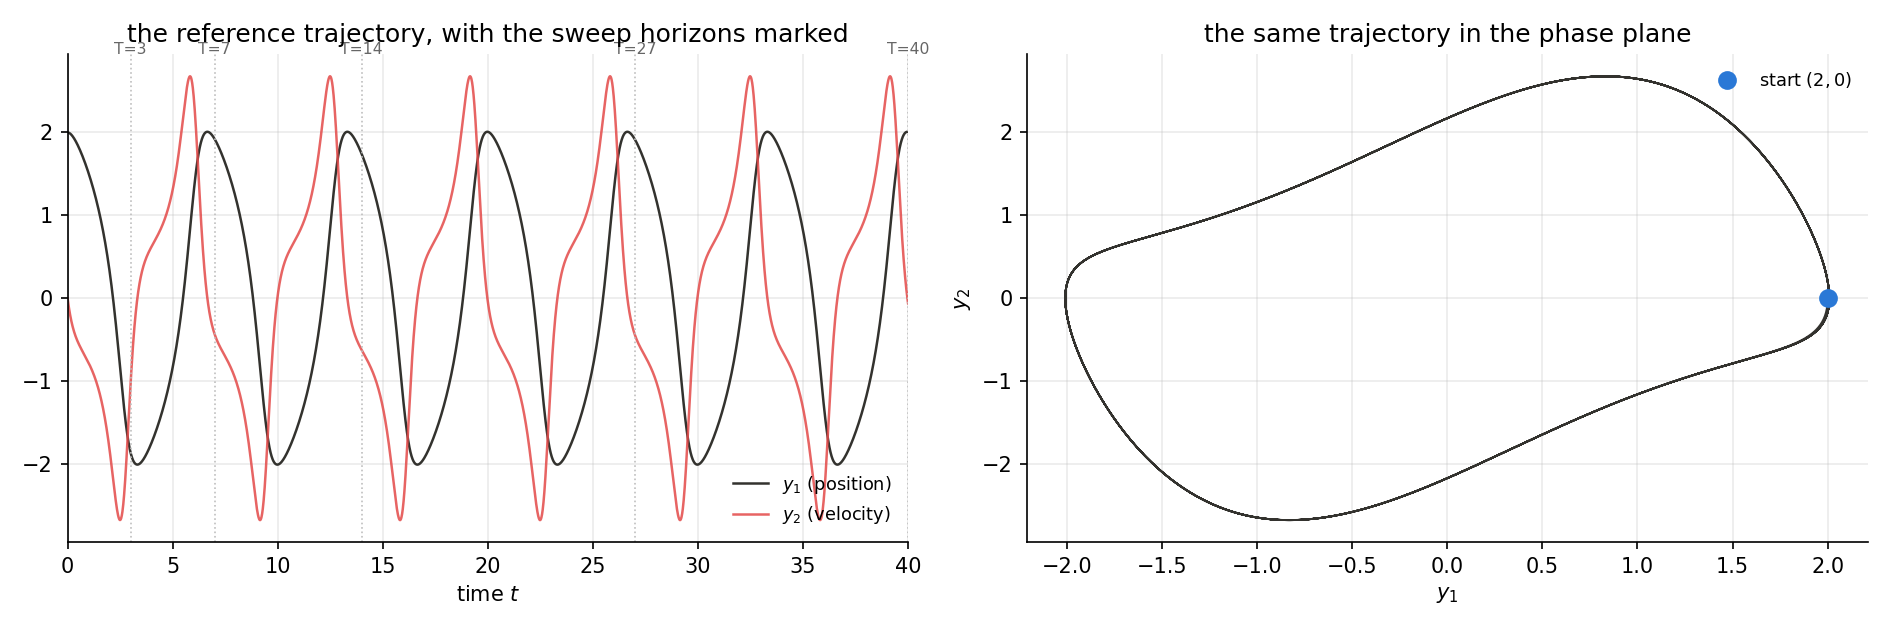
\includegraphics[width=\linewidth]{vdp_problem.png}
      \srcnote{Left: the reference from $(2,0)$ over six periods, with the five
        training horizons of the continuous-time experiments marked. Right: the
        same trajectory in the phase plane, the closed loop to be learned.}
    \end{column}
    \begin{column}{0.38\textwidth}
      \textbf{Verified, not asserted}
      \begin{enumerate}\small
        \item Convergence order, as the slope of global error against step size
              on three problems with closed-form solutions: measured
              \hl{$6.06$, $6.27$, $5.75$} against the theoretical $6$.
        \item Step-halving self-consistency reaches a rounding floor of
              $6.4\times10^{-14}$ below $h \approx 5\times10^{-3}$, so at the
              working step the truncation error is beneath double-precision
              rounding.
        \item Period \hl{$6.663287$} against the accepted $6.6633$.
        \item Closure of the limit cycle onto itself after one full period:
              $5.6\times10^{-14}$.
      \end{enumerate}
      \smallskip
      {\small Eight starting points integrated to $t = 40$. Used only for
       scoring, never for training, with the single deliberate exception of the
       data-trained twin. Where a network's evaluation times fall between stored
       samples the integrator is re-run to stop exactly there; nothing is
       interpolated.}
    \end{column}
  \end{columns}
\end{frame}

% ---- 23b: the local pipeline (added 2026-09-06) --------------------------
\begin{frame}[shrink=25]{Before the official sample: the full LHCb simulation and reconstruction chain, run locally}
  \vspace{1mm}
  \begin{columns}[T]
    \begin{column}{0.5\textwidth}
      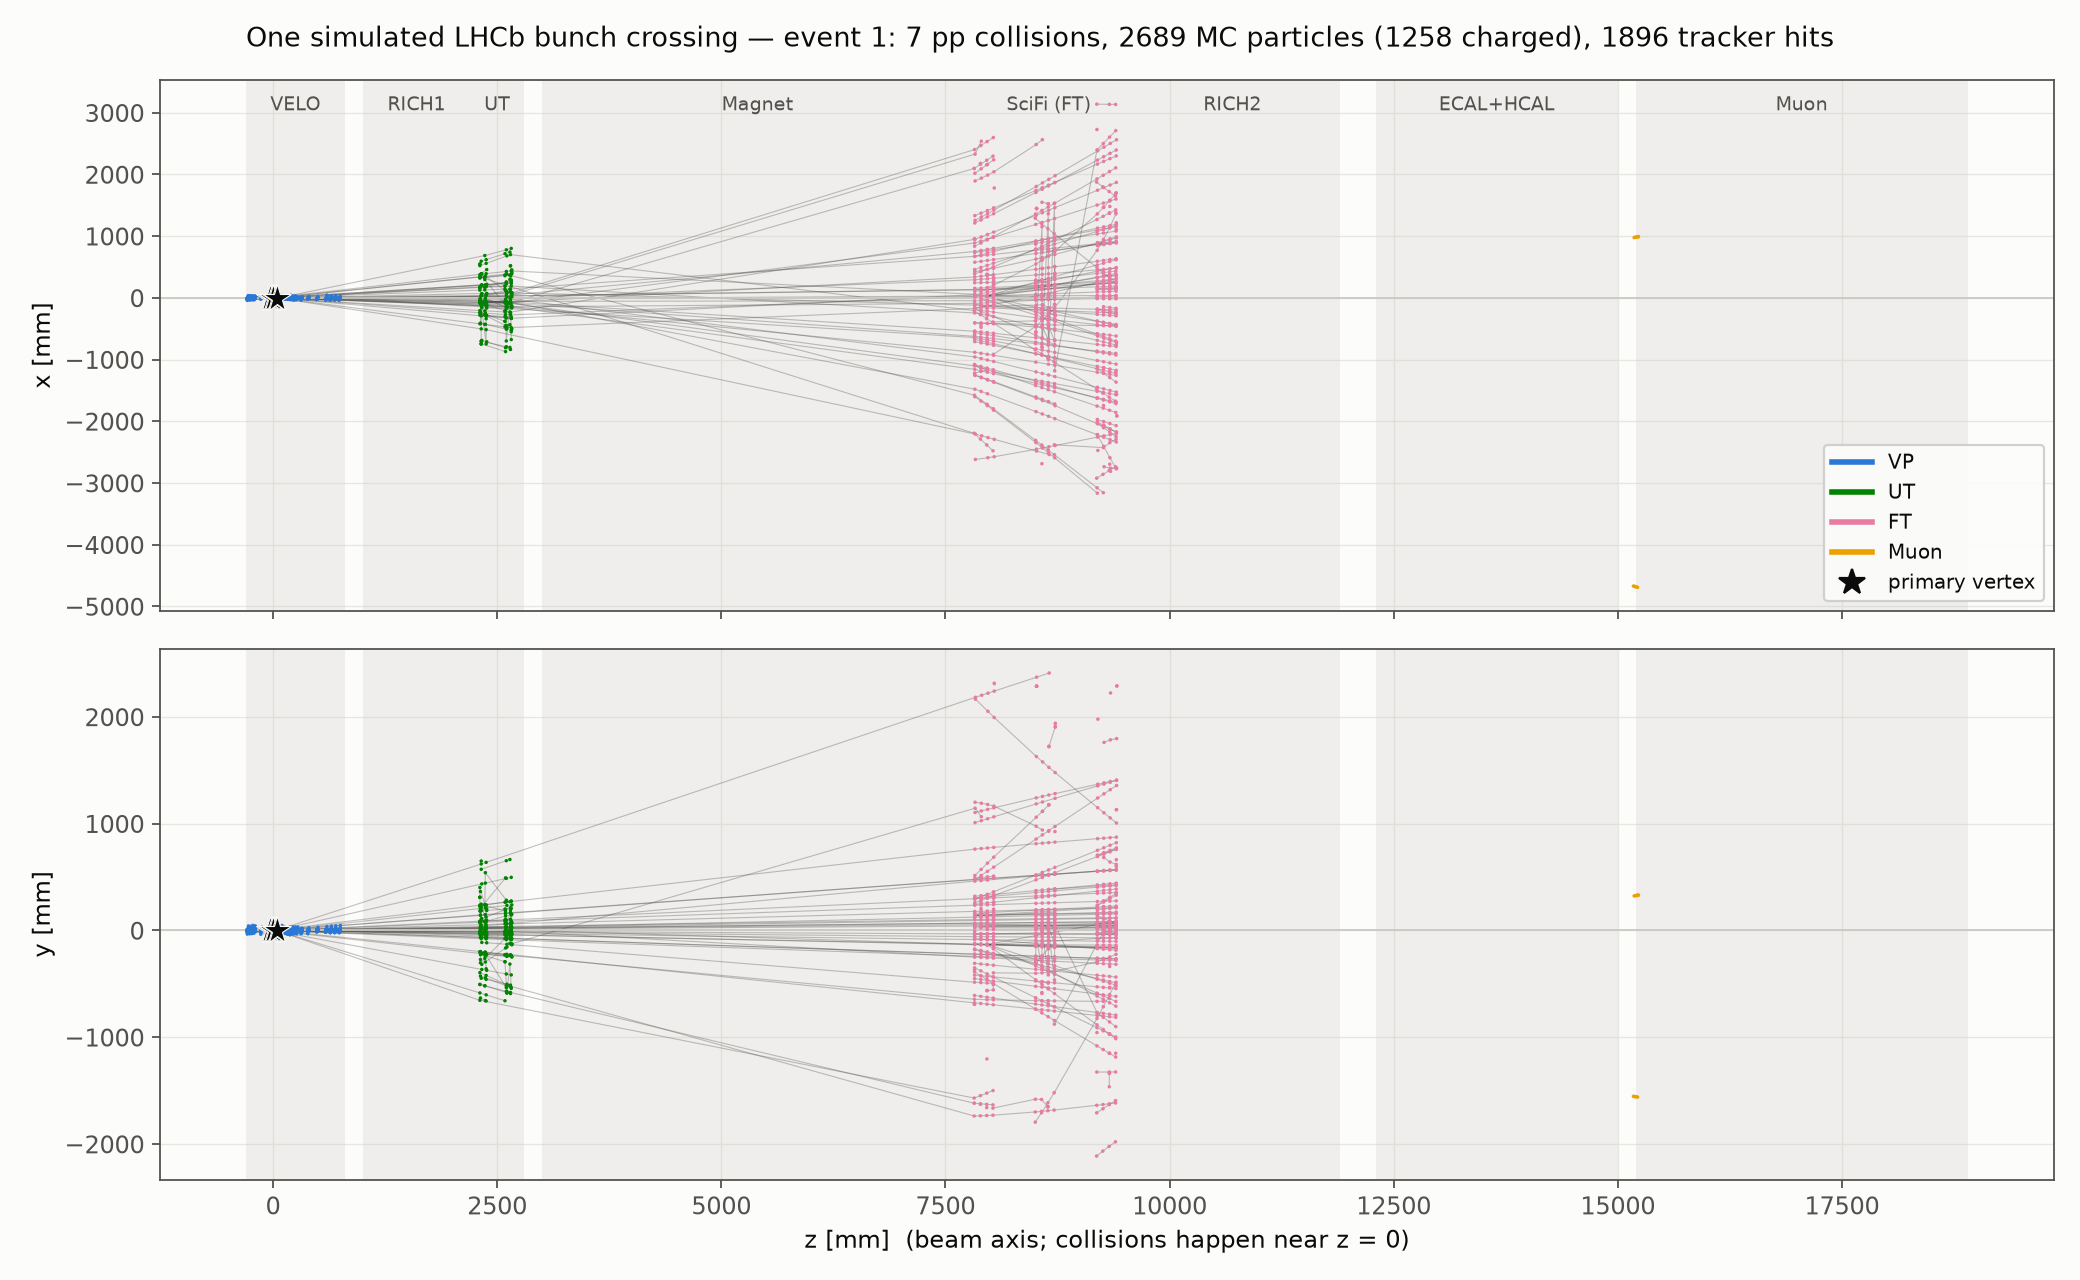
\includegraphics[width=\linewidth]{lhcb_event_display.png}
      \srcnote{One simulated minimum-bias event from the local chain: truth
        hits by subdetector, the magnet region marked. Everything in it was
        produced at Nikhef with no grid, eos or kerberos dependency.}
    \end{column}
    \begin{column}{0.48\textwidth}
      \textbf{The chain, proven end to end before any network was trained}
      \begin{itemize}\small
        \item Gauss v61r0p2, 2024 conditions and geometry, to Boole v48r0, to
              Moore v59r4: the HLT2 light reconstruction with its truth
              checkers, and HLT1 through Allen in Gaudi.
        \item On five events: long-track efficiency $87.4\%$, purity
              $99.4\%$, ghost rate $4.8\%$, the numbers the production
              checkers print, so the local chain reproduces the real
              reconstruction.
        \item A bulk run of $100$ events followed, with a first event-derived
              training set of $166{,}802$ rows.
        \item One root-caused gotcha worth keeping: Boole must write the
              \emph{extended} digitisation. The default output leaves dangling
              truth links and the Moore checkers segfault on it.
      \end{itemize}
      \smallskip
      \fbox{\parbox{0.93\textwidth}{\small On 21 July the training population
        was switched to the official simulation sample on the next slide, not
        because the chain was wrong but because small configuration errors in
        home-grown generation cause large and silent problems, and provenance
        has to be beyond argument. The chain remains the tool for reading
        reconstruction output and for the eventual validation inside Moore.}}
      \srcnote{Write-up: ``The data, figure by figure'' (Notion, Provisional).
        Repository: \texttt{Data\_generation\_exploration/First\_Pass}.}
    \end{column}
  \end{columns}
\end{frame}

% ---- 24 ------------------------------------------------------------------
\begin{frame}[shrink=25]{LHCb data: 323,533 legs of four kinds, harvested from an official sample}
  \vspace{1mm}
  \begin{columns}[T]
    \begin{column}{0.46\textwidth}
      \resizebox{\linewidth}{!}{\footnotesize
      \begin{tabular}{@{}clrr@{}}
        \toprule
        leg & what it is & typical step & rows \\
        \midrule
        A & vertex fetch & $341\mm$, backward & $49{,}014$ \\
        B & cross-magnet & $5175\mm$, both ways & $41{,}398$ \\
        C & plane-to-plane & $70\mm$, forward & $205{,}887$ \\
        D & downstream to vertex & $-8.6$ m & $27{,}234$ \\
        \midrule
        \multicolumn{2}{@{}l}{total} & &  $323{,}533$ \\
        \multicolumn{2}{@{}l}{split by particle, seed $20260718$}
          & \multicolumn{2}{r}{$258{,}857 / 32{,}389 / 32{,}287$} \\
        \bottomrule
      \end{tabular}}
      \smallskip

      {\small The harvest: dump the simulation truth; turn each tracker hit into
       a state with position, local slopes and truth momentum; form legs from
       each particle's own geometry; label by fourth-order Runge--Kutta at
       $5\mm$ \bad{with the magnet-down map (the sample is up; see the next
       slide)}; split by particle, because legs from one particle are highly
       correlated and splitting by leg would leak.
       \smallskip

       Type D is built and labelled but \hl{never trained on}: it is an
       out-of-training test by construction.
       \smallskip

       Official simulation, 2024 minimum-bias, $200$ events from five of eight
       files mirrored locally. A deliberate policy change on 21 July: small
       configuration errors in home-grown generation cause large and silent
       problems.}
    \end{column}
    \begin{column}{0.52\textwidth}
      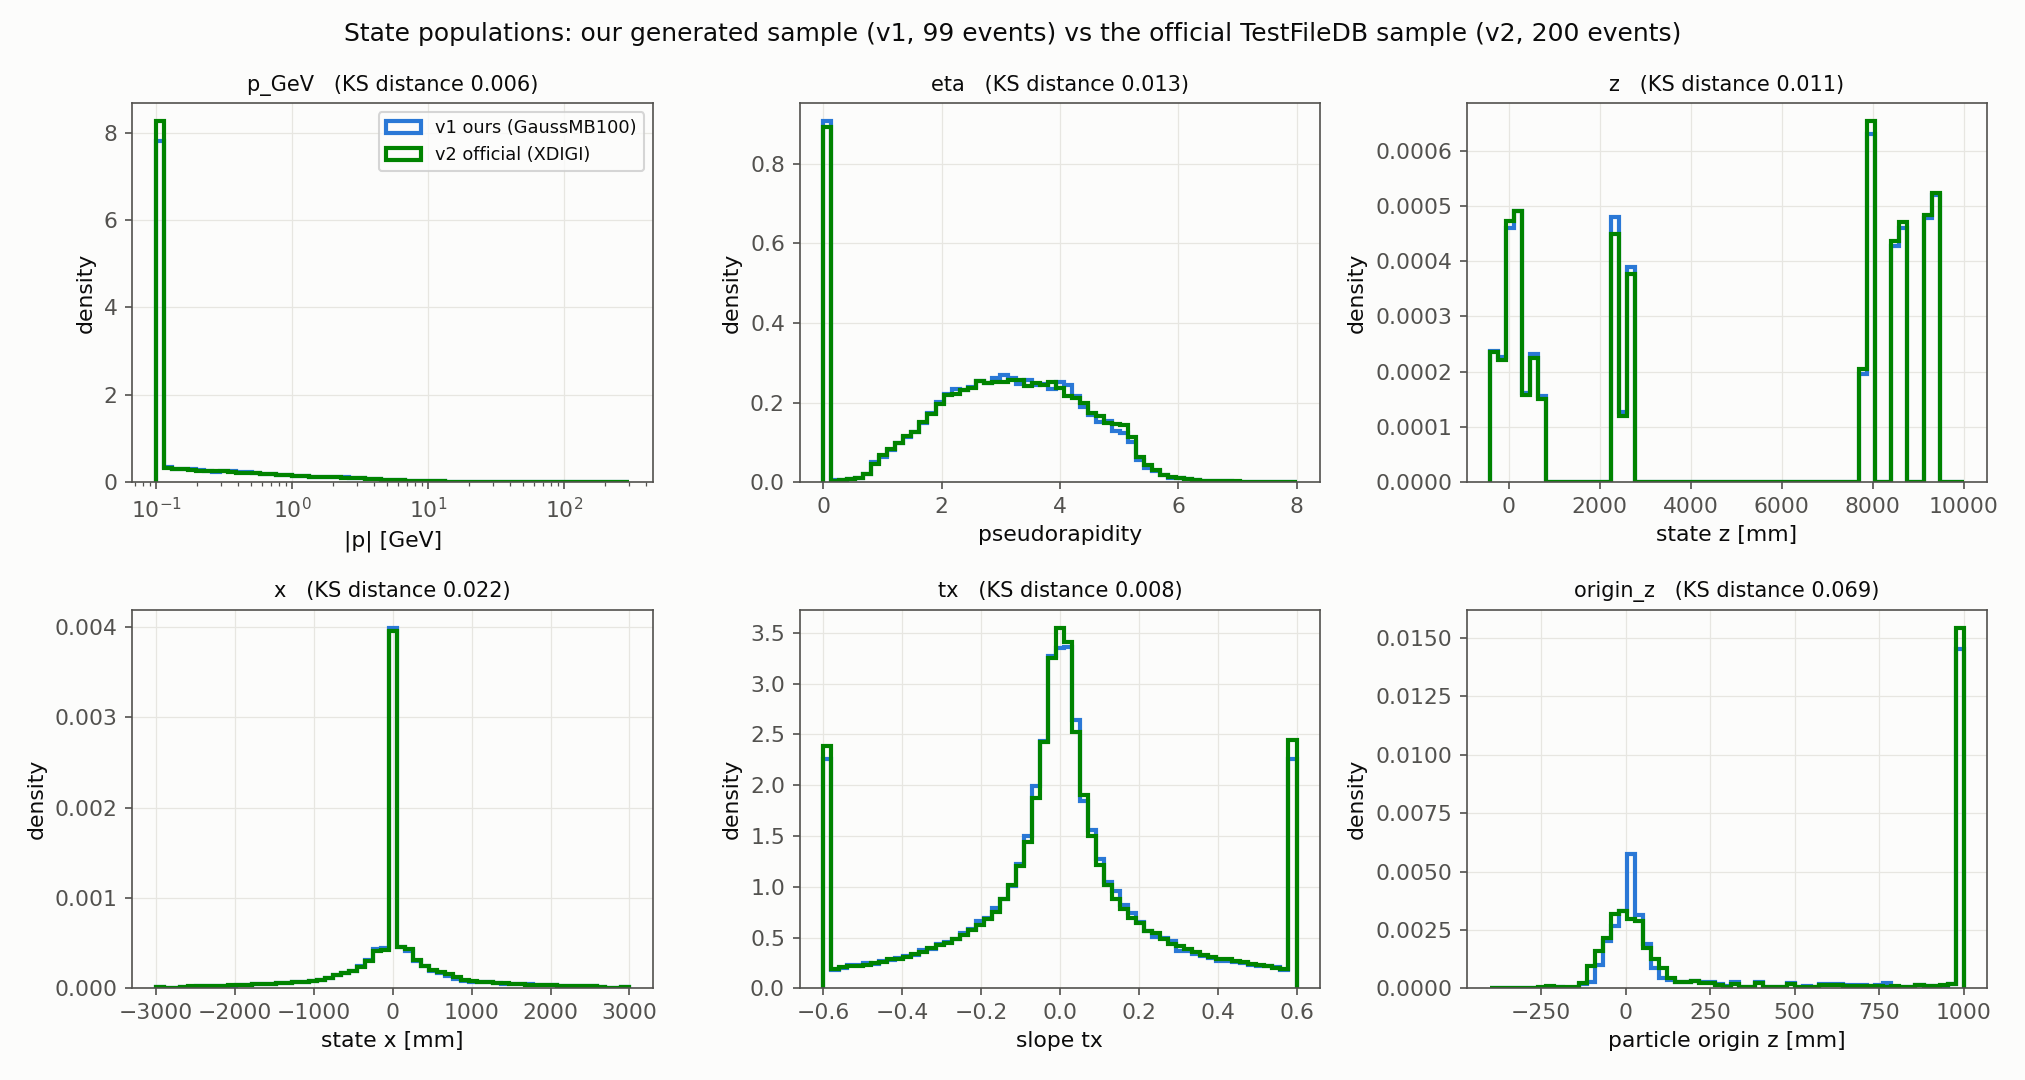
\includegraphics[width=\linewidth]{lhcb_population.png}
      \srcnote{The harvested population against the in-house sample it replaced:
        momentum, pseudorapidity, the $z$ of the harvested states, transverse
        position, slope, and the $z$ of the production point, with
        Kolmogorov--Smirnov distances printed. Distances $0.006$ to $0.069$, so
        switching sample changed the provenance of the population and not its
        physics. The three clusters in the $z$ panel are the detector itself.}
    \end{column}
  \end{columns}
\end{frame}

% ---- 25b  (correction slide, added 2026-09-07) ---------------------------
\begin{frame}[shrink=25]{Correction found last night: the sample is magnet-up}
  \vspace{1mm}
  \begin{columns}[T]
    \begin{column}{0.42\textwidth}
      {\footnotesize The conditions tag \texttt{sim-20231017-vc-mu100} is
       \bad{magnet-up}. Established 6 September while building the
       magnet-to-magnet data set: propagate each particle's forward
       cross-magnet leg and compare with that particle's \emph{own} real first
       SciFi state, on $15{,}257$ particles.}
      \smallskip

      \resizebox{\linewidth}{!}{\footnotesize
      \begin{tabular}{@{}lrr@{}}
        \toprule
        forward leg vs the real state & v8r1.up & v8r1.down \\
        \midrule
        median miss, all $15{,}257$ & \hl{$1.73\mm$} & $883\mm$ \\
        \quad $1$--$2$ GeV & $14.8\mm$ & $3973\mm$ \\
        \quad $25$--$200$ GeV & $0.28\mm$ & $169\mm$ \\
        bend sign correct & \hl{$100.0\,\%$} & \bad{$0.0\,\%$} \\
        legs leaving the field map & $0\,\%$ & $2\,\%$ \\
        \bottomrule
      \end{tabular}}
      \smallskip

      {\footnotesize The two maps are exact negatives, so polarity changes only
       the sign of the bend. \bad{Every July and Block A label and score used
       the down map}: the training set's $Y$ column, the frozen-leg
       experiments, the general-leg and residual experiments.}
    \end{column}
    \begin{column}{0.56\textwidth}
      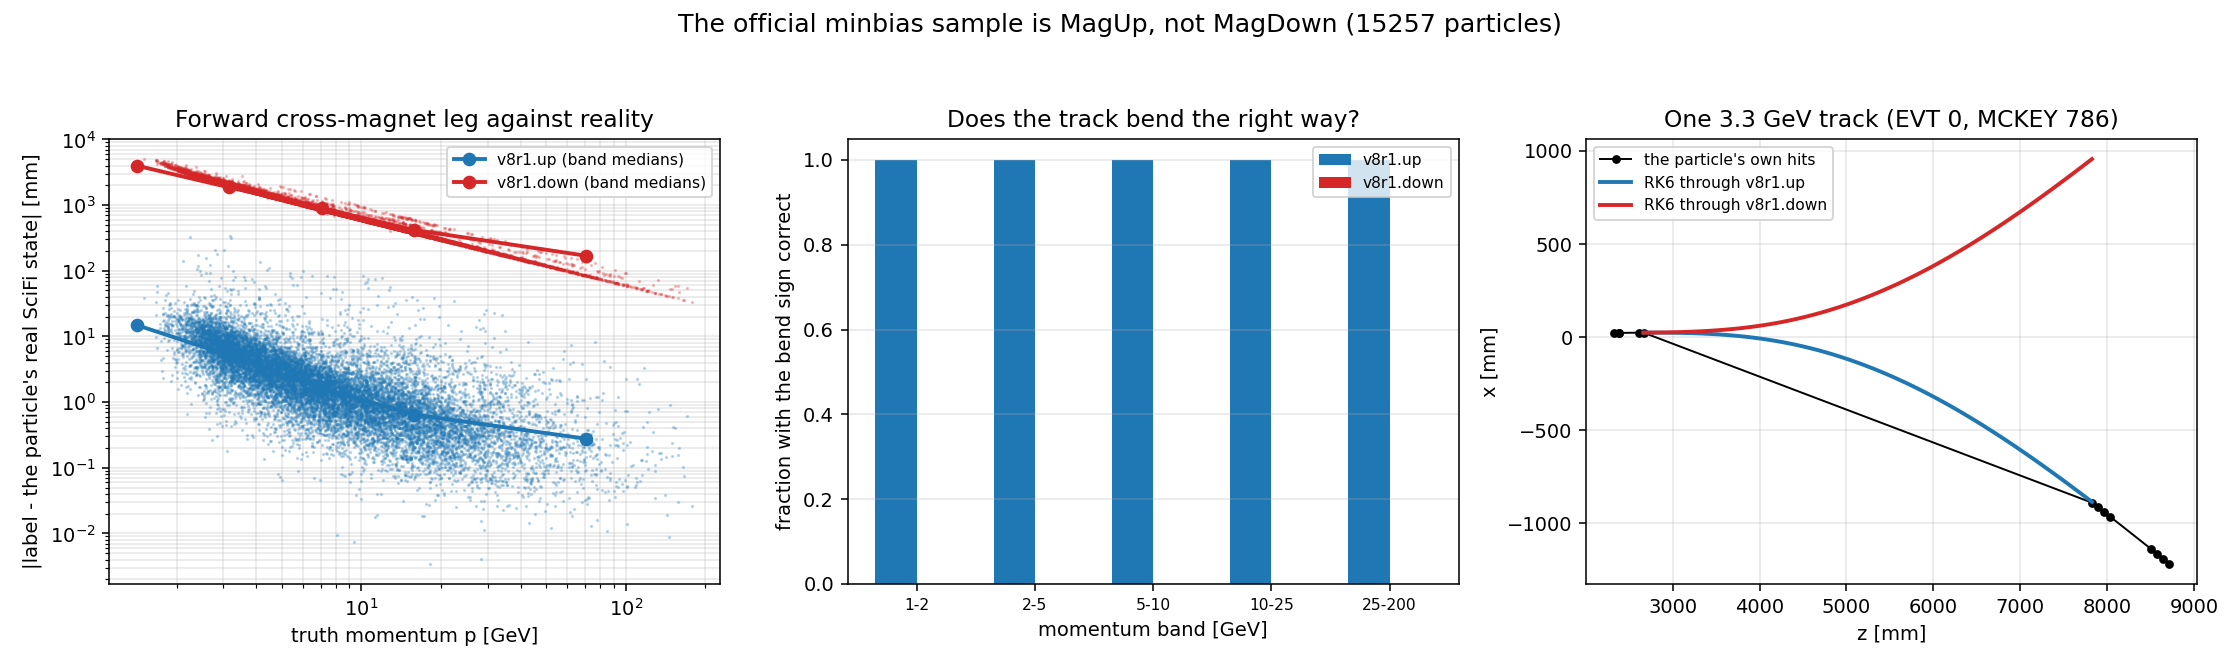
\includegraphics[width=\linewidth]{lhcb_field_polarity.png}
      \srcnote{Left: the forward cross-magnet leg against the particle's own
        real first-SciFi state, per particle, both maps, with band medians.
        Middle: the fraction of particles whose bend has the right sign, by
        momentum band. Right: one $3.3$ GeV track, its own hits and the
        reference path through each map.}
      \vspace{1mm}

      {\footnotesize\textbf{Four consequences, no more and no less.}
      \begin{itemize}\setlength{\itemsep}{2pt}
        \item \hl{Every method conclusion stands.} Each experiment compared a
              network against the same equations and the same engine:
              scheme-limited against network-limited, the optimisation-limited
              floor, the residual redesign, chaining.
        \item \bad{Any statement that those labels are where the simulated
              particle went is wrong}, and the material-floor gate G2 must be
              re-read on the up map.
        \item The magnet-up experiment is \bad{not ``a polarity with no
              labels''} but the sample's true polarity, and the only one here
              scored against the physically right field. Its result (same
              floor, $229$ against $222\um$) is unchanged; its framing is.
        \item The new magnet-to-magnet set, the fine reference and the tables
              in progress are \hl{built on the up map}.
      \end{itemize}}
    \end{column}
  \end{columns}
\end{frame}

% ---- 25 ------------------------------------------------------------------
\begin{frame}[shrink=25]{Four gates on the labels, and the one percent of states that carried half the loss}
  \framesubtitle{}
  \vspace{1mm}
  \begin{columns}[T]
    \begin{column}{0.44\textwidth}
      \centering
      \resizebox{\linewidth}{!}{\small
      \begin{tabular}{@{}clr@{}}
        \toprule
        gate & what it checks & result \\
        \midrule
        G1 & closure: propagate forwards, then backwards & median $1.4$ nm \\
        G2 & truth: against the particle's own next hit & median $22\um$ \\
           & \quad the same, above $5$ GeV & $6.3\um$ \\
           & \quad the same, below $2$ GeV & $86\um$ \\
        G3 & step: repeat the integration at $1\mm$, not $5\mm$ & median $8.9$ nm \\
        G4 & conservation: $\qop$ passes through unchanged & exact \\
        \bottomrule
      \end{tabular}}
      \smallskip

      {\small G2 defines the scope of the project. The label disagrees with the
       real next hit by an amount growing as $1/p$, the signature of multiple
       scattering. That residual is not an error in the labels; it is the
       material effect, deliberately outside the surrogate's remit.
       \bad{G2 was measured with down-map labels and must be re-read on the up
       map (previous slide).}}
    \end{column}
    \begin{column}{0.54\textwidth}
      \textbf{The fiducial requirement, and why it is the portability lesson}
      \begin{itemize}\small
        \item First run against the official sample: the physics loss appeared
              far worse than the twin, $403$ to $595\um$ against $175$ to
              $213\um$.
        \item Cause: \hl{$21$ of $2000$ training states}, one percent, are soft
              tracks of $1.2$ to $1.5$ GeV that bend so hard they leave the
              field map, past $|x| = 4$ m, outside the LHCb acceptance as well.
              Those $21$ states carried \hl{half of the entire physics loss};
              the top one percent carried $68$ to $78$ percent.
        \item \hl{The asymmetry is structural.} The physics loss evaluates the
              field where the network proposes, so a trajectory outside the map
              is asked to satisfy equations built on a clamped, meaningless
              field. The twin never touches the field: it fits labels computed
              with the same clamped field and absorbs the pathology silently.
        \item With the requirement in place, runs stopped stalling at a plateau,
              taking $147$ to $152$ restarts instead of $57$ to $72$, and the
              training loss fell from about $1.1\times10^{-4}$ to
              $8.3\times10^{-6}$, the same range as the twin.
      \end{itemize}
    \end{column}
  \end{columns}
\end{frame}

% =========================================================================
% V. RESULTS, VAN DER POL
% =========================================================================

% ---- 26 ------------------------------------------------------------------
\begin{frame}[shrink=25]{The continuous-time construction is excellent below one period and collapses beyond it}
  \vspace{1mm}
  \begin{columns}[T]
    \begin{column}{0.52\textwidth}
      \centering\small
      \begin{tabular}{@{}cccll@{}}
        \toprule
        $T$ & periods & $N$ & rel.\ $L_2$ (median) & final loss \\
        \midrule
        3  & 0.45 & 60  & $3.8\times10^{-5}$ & $1.4$--$2.0\times10^{-7}$ \\
        7  & 1.05 & 140 & $6.6\times10^{-4}$ & $2.3\times10^{-6}$--$2.8\times10^{-5}$ \\
        14 & 2.10 & 280 & \bad{$0.79$} & $\approx 6\times10^{-2}$ \\
        27 & 4.05 & 540 & \bad{$0.90$} & $\approx 3\times10^{-2}$ \\
        40 & 6.00 & 800 & \bad{$0.94$} & $2.1$--$4.8\times10^{-2}$ \\
        \bottomrule
      \end{tabular}
      \smallskip

      {\small Collocation density fixed at $20$ points per unit time; medians
       over three seeds. Best and worst seeds at $T = 14$ are $0.789$ and
       $0.805$: \hl{the seeds agree to two decimal places}, so the failure is
       systematic and not an initialisation accident.
       \smallskip

       Below one period this is at or better than the accuracy the source work
       reports for its own continuous-time demonstrations,
       $1.97\times10^{-3}$ and $6.7\times10^{-4}$. Unsurprising for a two-state
       oscillator against partial differential equations, but it confirms the
       machinery is correctly built.}
    \end{column}
    \begin{column}{0.46\textwidth}
      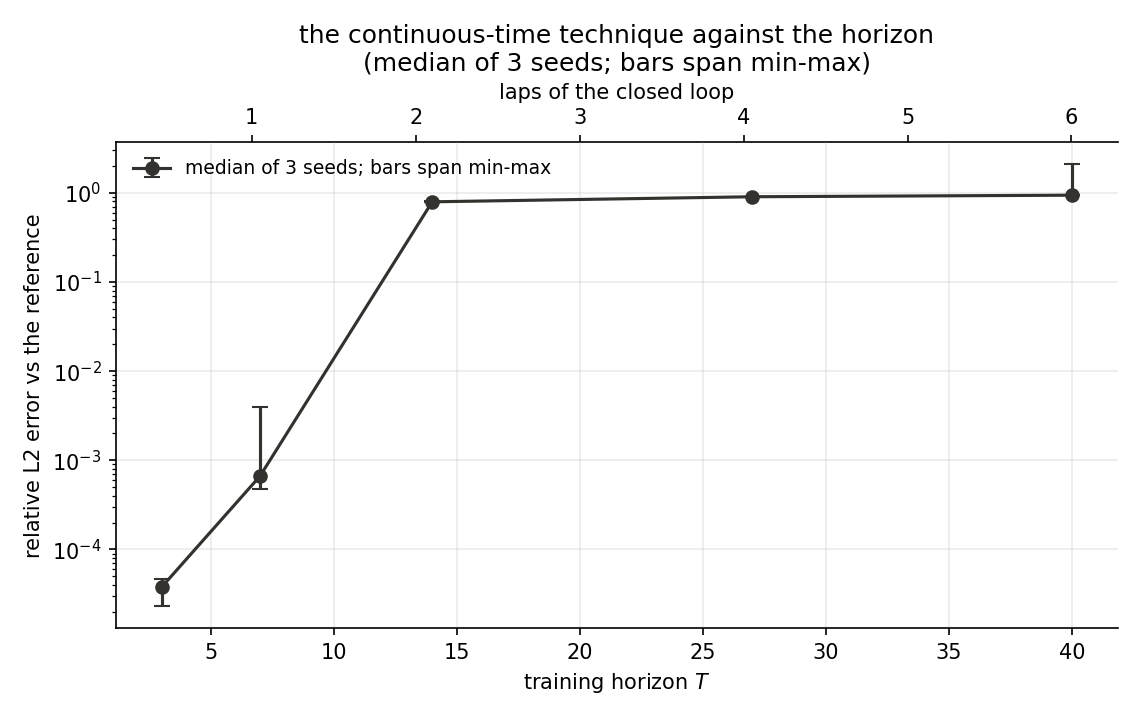
\includegraphics[width=0.86\linewidth]{vdp_cliff.png}\\[1mm]
      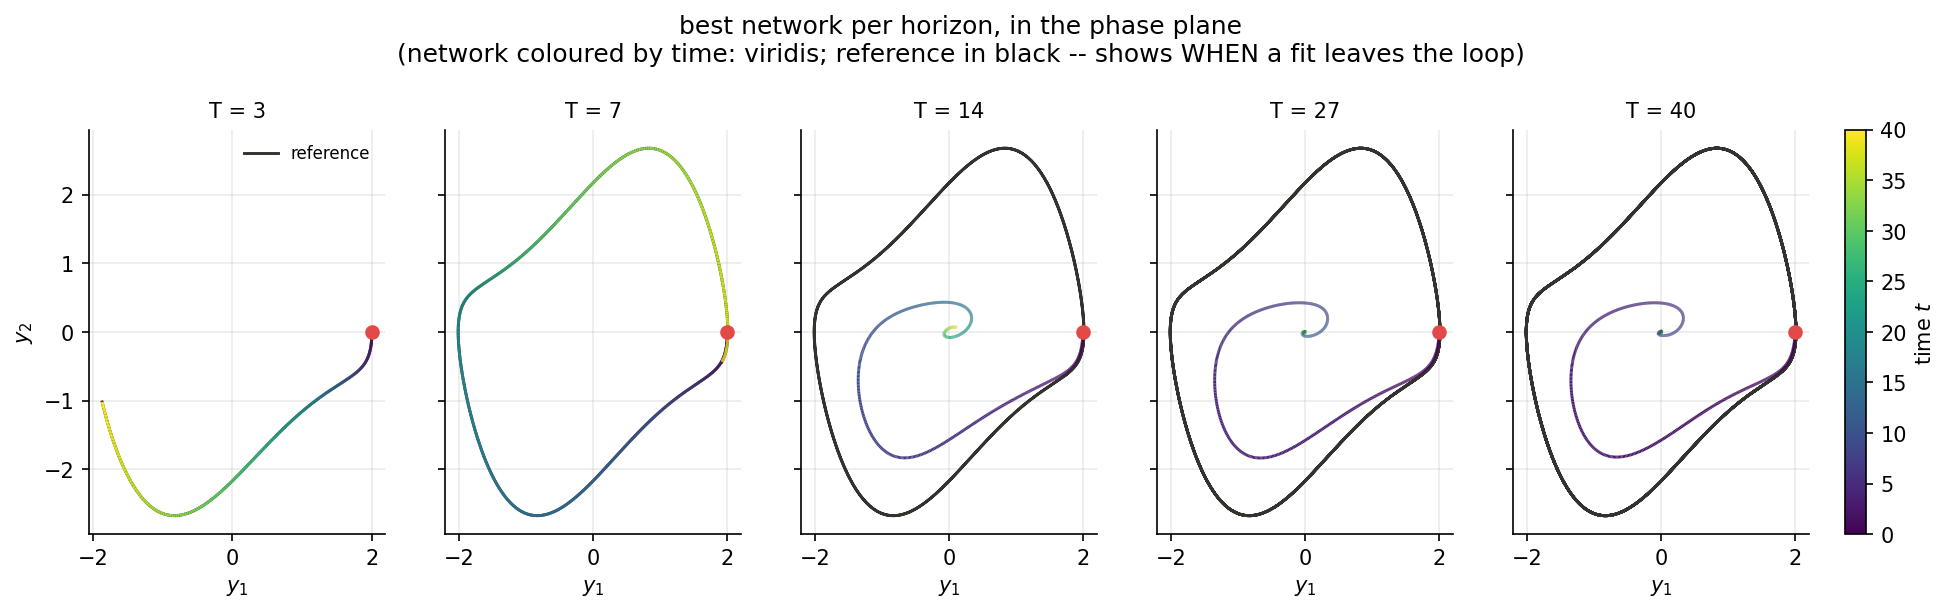
\includegraphics[width=0.86\linewidth]{vdp_phase_collapse.png}
      \srcnote{Top: relative $L_2$ against training horizon, median of three
        seeds with min to max whiskers. Bottom: the failed fits in the phase
        plane, best seed per horizon. Past one period the fit abandons the
        closed loop and spirals into the origin, \emph{against} the direction of
        the true flow.}
    \end{column}
  \end{columns}
\end{frame}

% ---- 26b: the classical anchor (added 2026-09-06) -------------------------
\begin{frame}[shrink=25]{A classical anchor at the same step: explicit is unusable, implicit is fine, and the network beats implicit where it works}
  \vspace{1mm}
  \begin{columns}[T]
    \begin{column}{0.5\textwidth}
      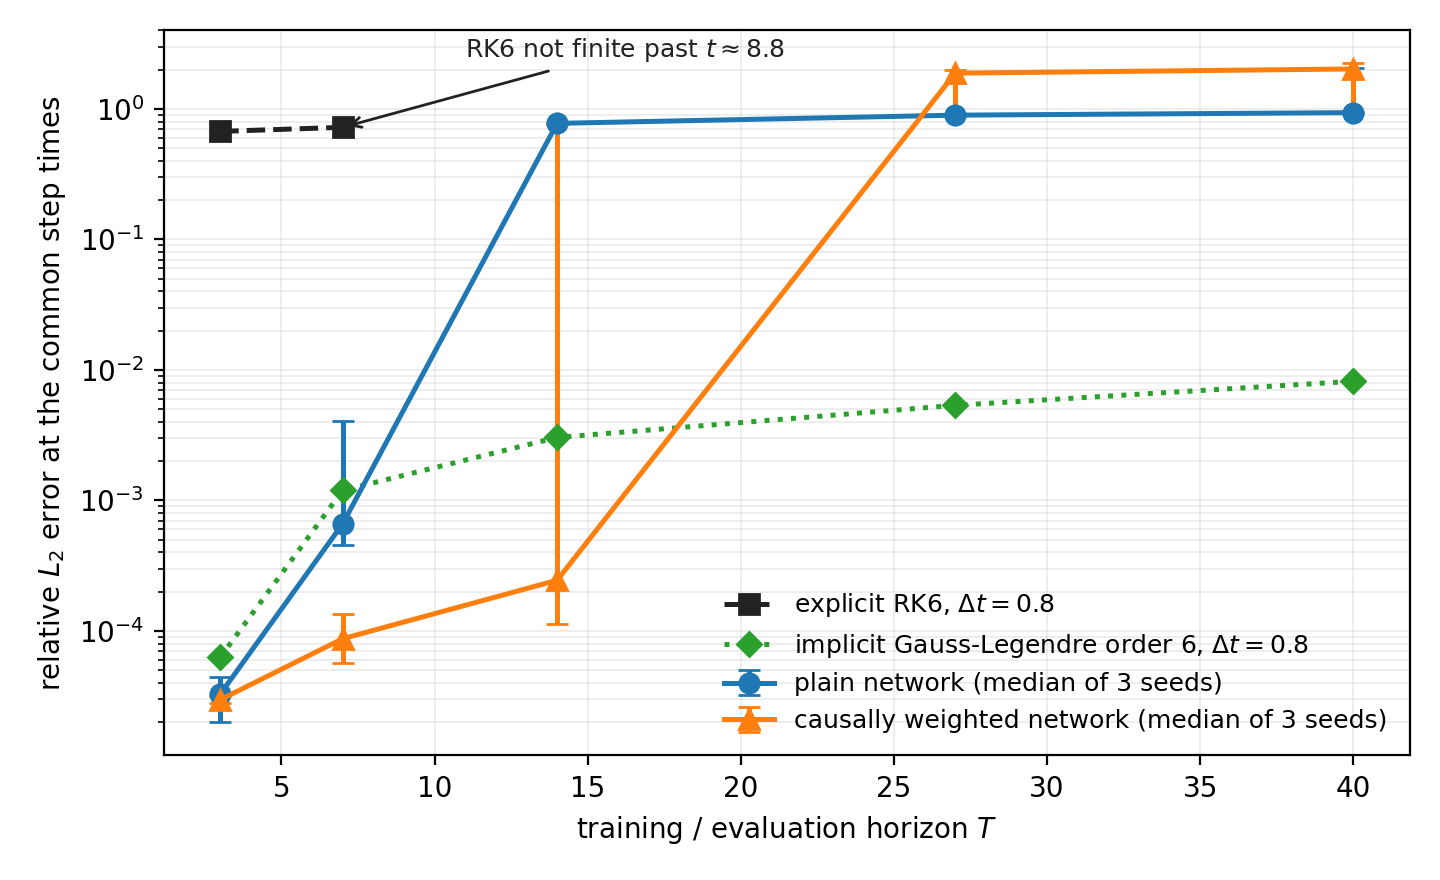
\includegraphics[width=\linewidth]{vdp_rk6_comparison.png}
      \srcnote{Two classical runs at the discrete-time study's step
        $\Delta t = 0.8$, chained from $(2, 0)$: the reference integrator's own
        seven-stage explicit order-6 tableau, and Gauss--Legendre with $q = 3$,
        also order 6, solved by root-finding. Both scored by the same relative
        $L_2$ at the common step times as the networks.}
    \end{column}
    \begin{column}{0.48\textwidth}
      \centering\footnotesize
      \begin{tabular}{@{}ccccc@{}}
        \toprule
        $T$ & explicit RK6 & implicit GL, order 6 & plain network & causal network \\
        \midrule
        3  & $0.67$ & $6.3\times10^{-5}$ & $3.3\times10^{-5}$ & $3.0\times10^{-5}$ \\
        7  & $0.72$ & $1.2\times10^{-3}$ & $6.6\times10^{-4}$ & $8.7\times10^{-5}$ \\
        14 & not finite & $3.0\times10^{-3}$ & \bad{$0.78$} & $2.5\times10^{-4}$ \\
        27 & not finite & $5.4\times10^{-3}$ & \bad{$0.90$} & \bad{$1.88$} \\
        40 & not finite & $8.2\times10^{-3}$ & \bad{$0.94$} & \bad{$2.03$} \\
        \bottomrule
      \end{tabular}
      \smallskip
      \begin{itemize}\small
        \item The explicit method at this step is outside its stable range: the
              state reaches $10^{21}$ by $t = 8$ and is not finite past $8.8$.
        \item The implicit member of the same family is stable at every horizon;
              beyond two periods it is the only method in the table that works.
        \item Within the networks' working range the network is the more
              accurate: $3.0\times10^{-5}$ against $6.3\times10^{-5}$ at
              $T = 3$, $2.5\times10^{-4}$ against $3.0\times10^{-3}$ at two periods.
      \end{itemize}
      \fbox{\parbox{0.93\textwidth}{\small Two separate questions. At a fine step
        classical integration beats every network here by orders of magnitude.
        At a coarse step of $0.8$ only \hl{implicit structure} takes the step
        accurately, solved classically as here or learned as in the
        discrete-time column.}}
    \end{column}
  \end{columns}
\end{frame}

% ---- 27 ------------------------------------------------------------------
\begin{frame}[shrink=25]{Causal weighting moves the cliff to two periods and turns silent failures into visible ones}
  \vspace{1mm}
  \begin{columns}[T]
    \begin{column}{0.5\textwidth}
      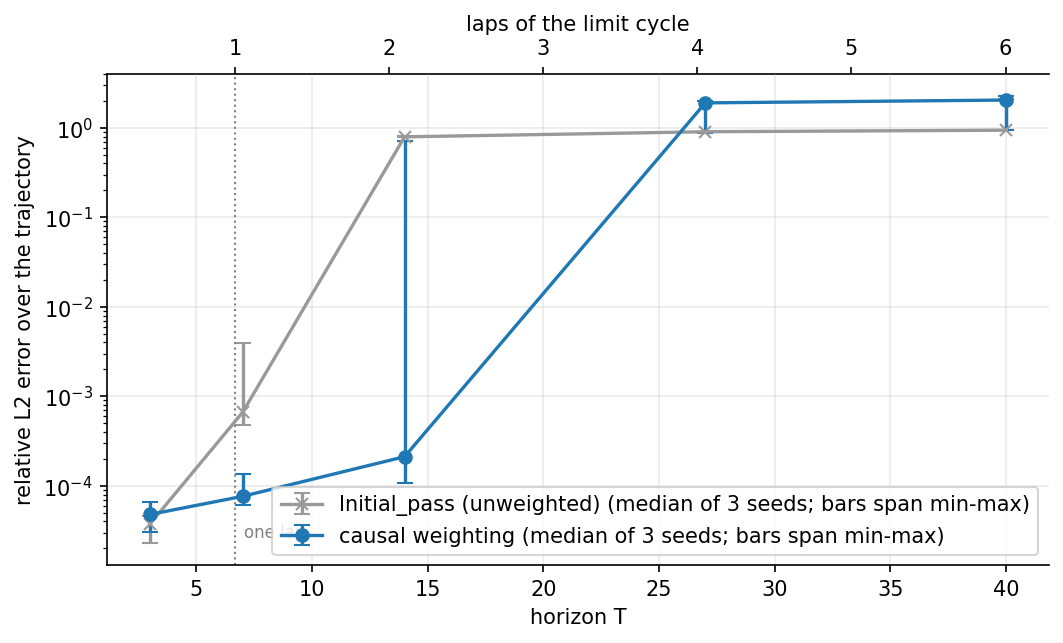
\includegraphics[width=\linewidth]{vdp_causal_compare.png}
      \srcnote{Same metric, same reference, same collocation density on both
        sides; the causally weighted runs add an Adam phase of up to $60{,}000$
        epochs before an identical final L-BFGS phase. Median of three seeds
        with min to max whiskers.}
    \end{column}
    \begin{column}{0.48\textwidth}
      \begin{itemize}\small
        \item At two periods, where the plain objective fails at $0.79$, causal
              weighting reaches \hl{$2.1\times10^{-4}$}: three to four orders of
              magnitude. In the capped measure the contrast is about seven
              orders, mean $\rho$ of $6.2\times10^{-1}$ against
              $4.0\times10^{-8}$.
        \item \hl{The essential difference is visibility.} These failures
              declare themselves: the minimum weight and the front position show
              it still mid-domain. The plain failures reported themselves as
              converged.
        \item One run at the epoch limit produced a second kind of silent
              failure, and it is the one that matters: \bad{training loss
              $9.7\times10^{-6}$ with error $0.71$}, an out-of-phase
              near-solution joined to the truth by a jump inside an unsampled
              interval, invisible both to the loss and to weights computed on
              the same grid.
        \item That single run is the empirical form of the splice theorem, found
              before I knew what it was.
      \end{itemize}
    \end{column}
  \end{columns}
\end{frame}

% ---- 27b: the resource axes (added 2026-09-06) ----------------------------
\begin{frame}[shrink=25]{The resource axes under the original protocol: 600 + 72 + 24 runs, and none of them moves the four-period wall}
  \vspace{1mm}
  \begin{columns}[T]
    \begin{column}{0.5\textwidth}
      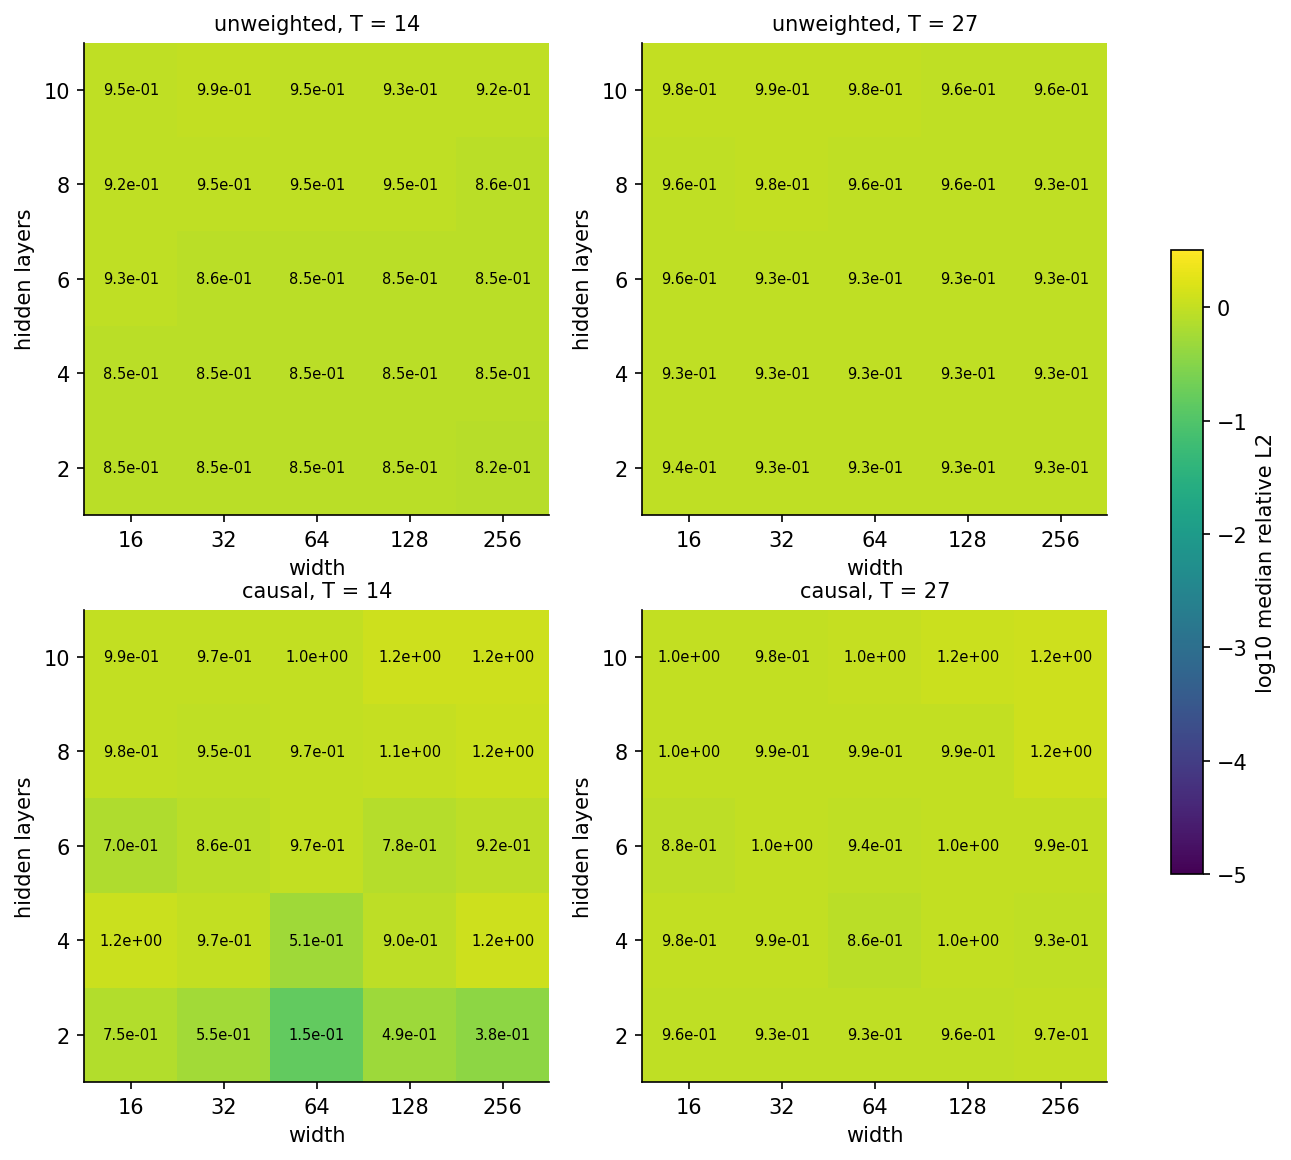
\includegraphics[width=\linewidth,height=0.36\textheight,keepaspectratio]{vdp_size_heatmaps.png}\\[1mm]
      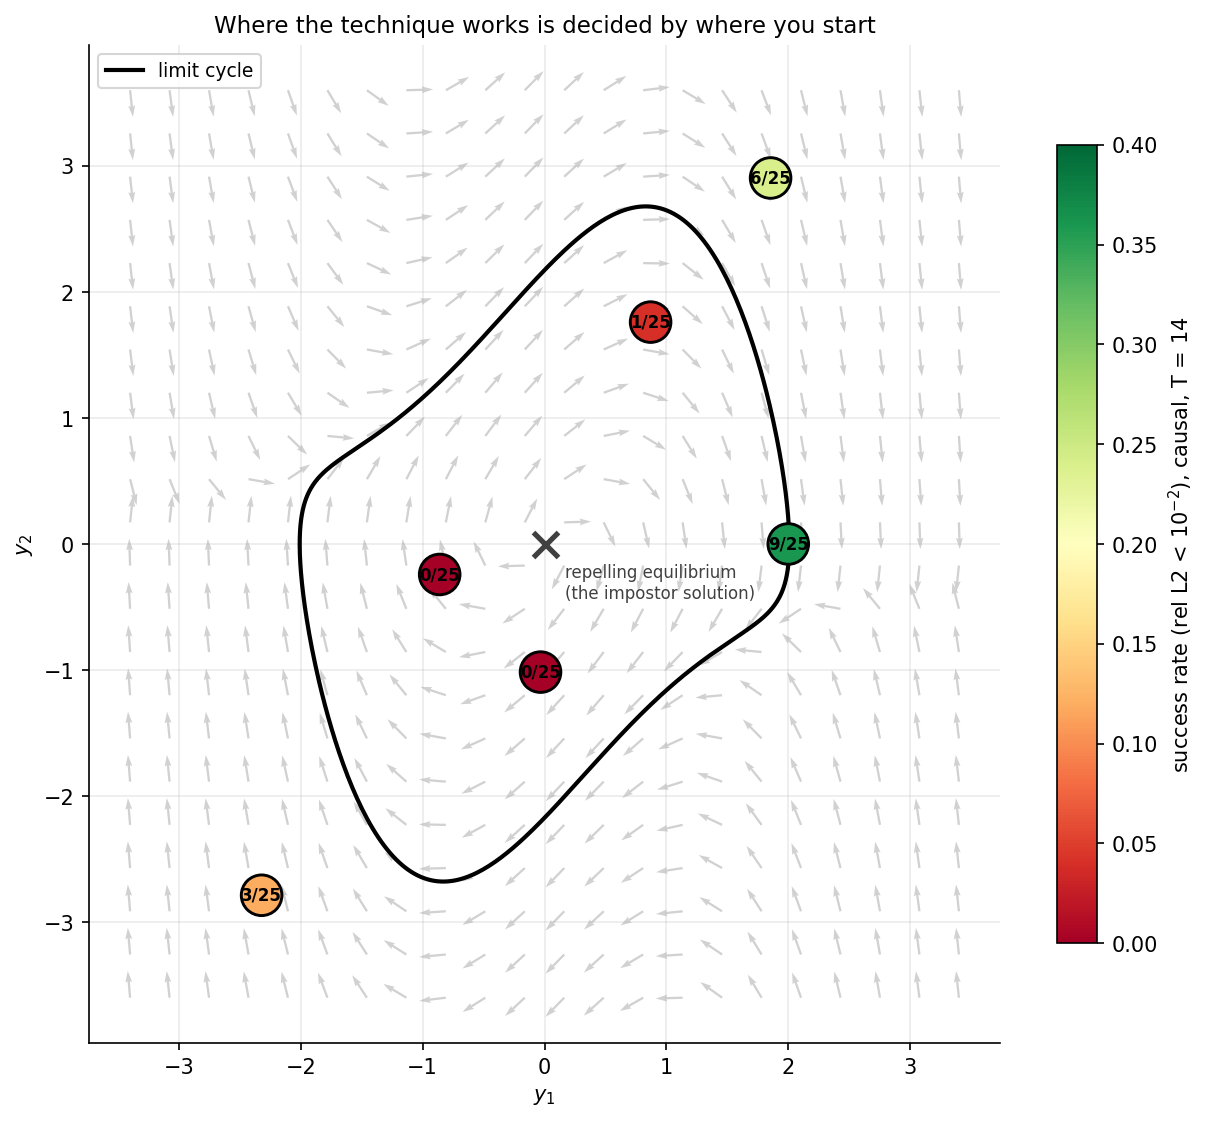
\includegraphics[width=0.49\linewidth,height=0.3\textheight,keepaspectratio]{vdp_success_map.png}\hfill
      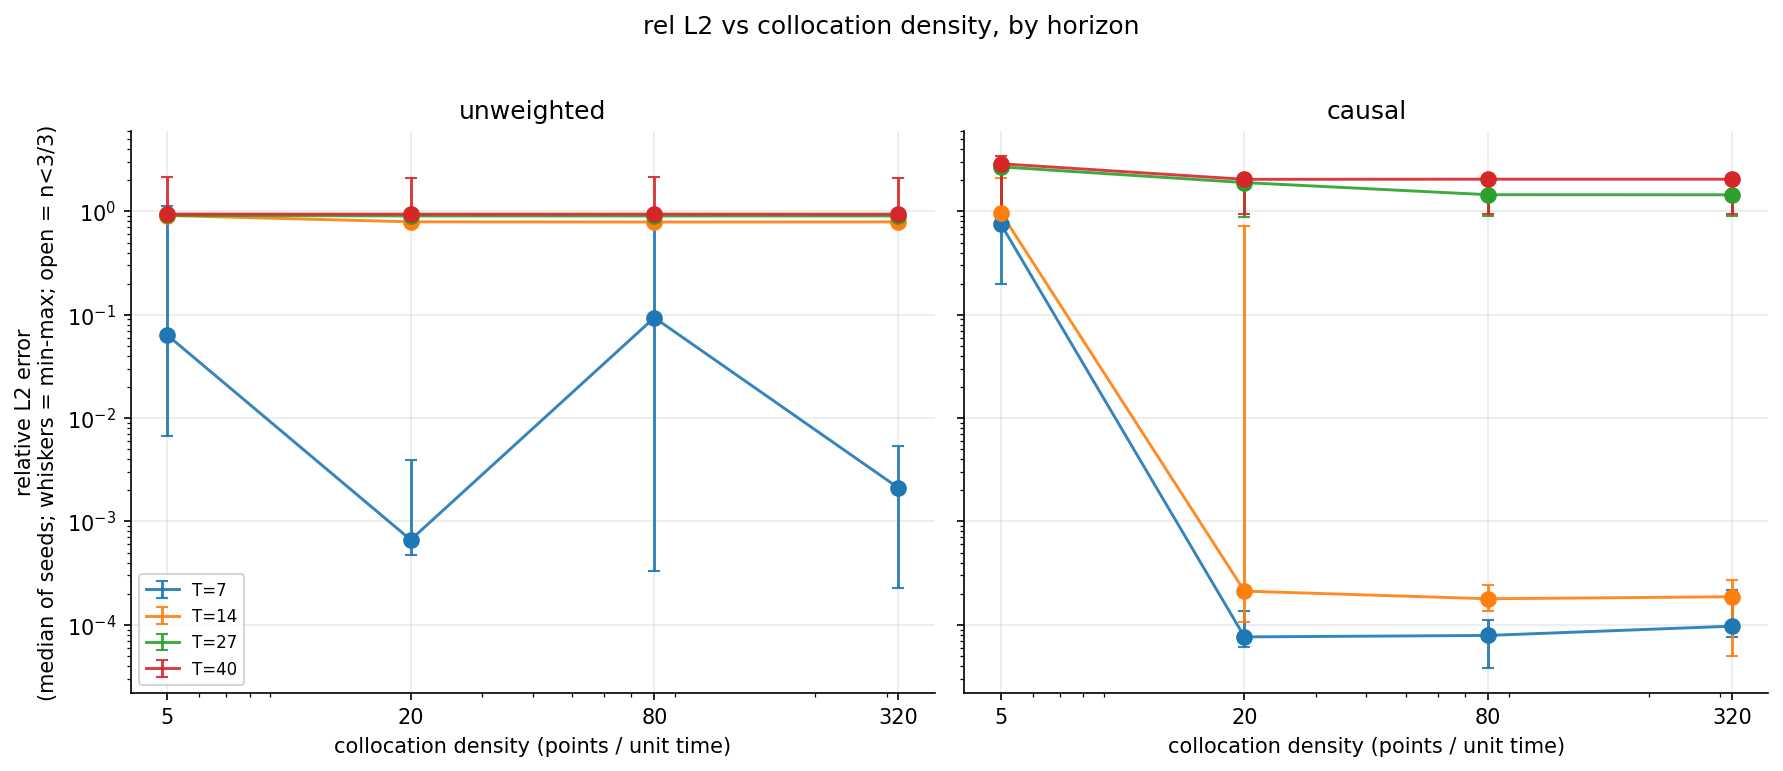
\includegraphics[width=0.49\linewidth,height=0.3\textheight,keepaspectratio]{vdp_density.png}
      \srcnote{Top: median relative $L_2$ by depth and width, both variants,
        two and four periods. Bottom left: the six starting states on the vector
        field, coloured by success at two periods. Bottom right: error against
        collocation density, 5 to 320 points per unit time.}
    \end{column}
    \begin{column}{0.48\textwidth}
      \begin{itemize}\small
        \item \hl{Network size and starting state, 600 runs}: 25 architectures,
              depth 2 to 10 and width 16 to 256, six starts, both variants, two
              and four periods. Size does not move the wall and added depth is
              harmful. What orders the outcomes is the start: success at two
              periods in \hl{19 of 150} causally weighted runs at the 1\% bar,
              concentrated on the outer starts, and at four periods in
              \bad{none of 300}.
        \item \hl{Collocation density, 72 runs}: a 64-fold range moves the
              plain medians at two, four and six periods by factors
              $1.15$, $1.01$, $1.003$. Causal weighting needs about 20 points
              per unit time for its weight condition to be informative, and no
              more.
        \item \hl{Collocation placement, 24 runs}: uniform, jittered, and 40
              extra points packed into the unsampled gap after $t = 0$ through
              which the starved runs escaped. Plugging the gap changes nothing.
      \end{itemize}
      \fbox{\parbox{0.93\textwidth}{\small All under the L-BFGS-only protocol.
        With training taken to a demonstrated plateau (slide on the two axes,
        later) density 80 lifts the plain objective at \emph{two} periods from
        5 to 10 of 10; the four-period wall stays. So the conclusion stands
        where it matters: resources change the price of the truth, not the
        price of a splice.}}
    \end{column}
  \end{columns}
\end{frame}

% ---- 28 ------------------------------------------------------------------
\begin{frame}[shrink=25]{The same networks fit four periods from data, so the objective fails and not the network}
  \vspace{1mm}
  \begin{columns}[T]
    \begin{column}{0.56\textwidth}
      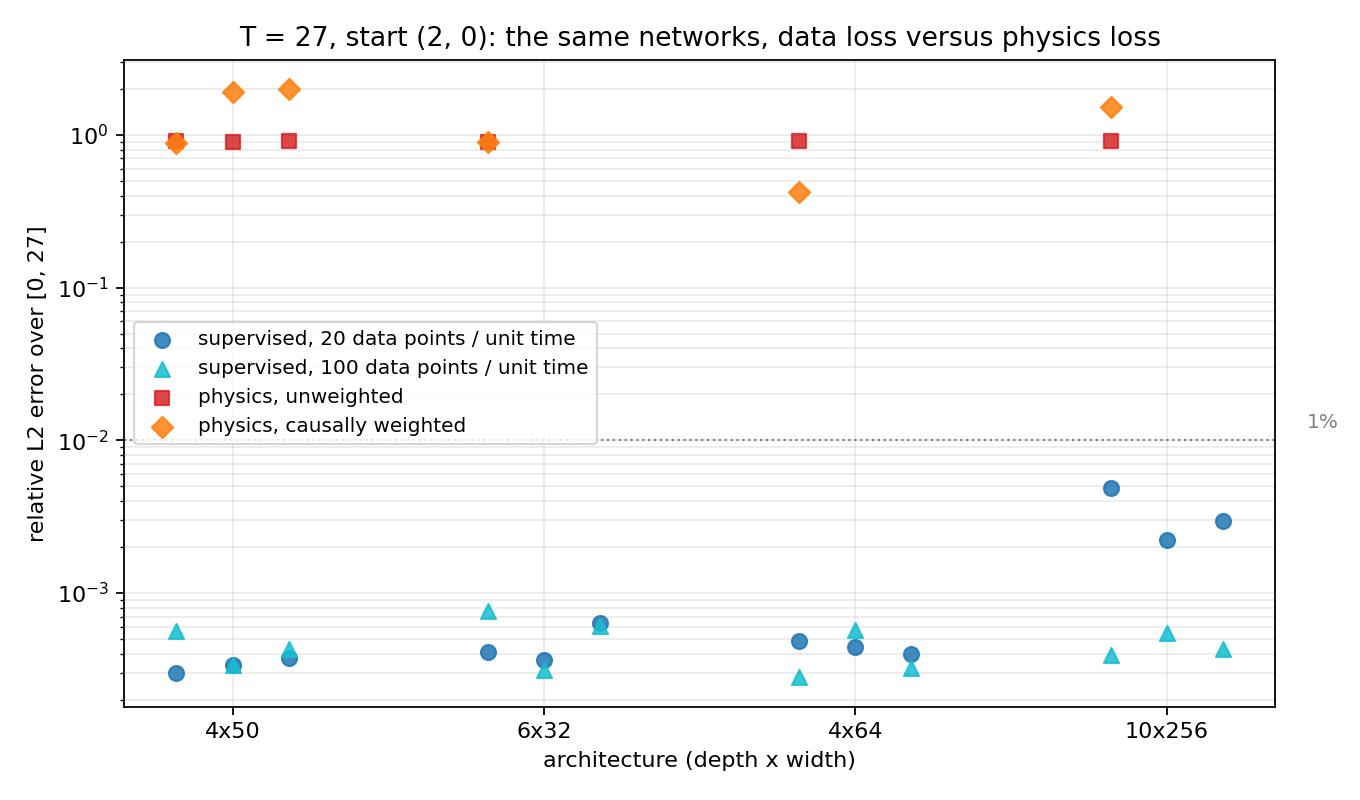
\includegraphics[width=\linewidth]{vdp_control_compare.png}
      \srcnote{Every supervised run at four periods, at both sample densities,
        against both physics variants, by architecture. The separation is three
        to four orders of magnitude with the network, the sample times and the
        optimiser caps held fixed.}
    \end{column}
    \begin{column}{0.42\textwidth}
      \textbf{The design}
      \begin{itemize}\small
        \item Same networks, same sample-time distribution, same optimiser, same
              caps, at four periods. \hl{Only the loss changed}: plain mean
              squared error to the known states, no residual anywhere.
        \item Four architectures ($4\times50$, $6\times32$, $4\times64$,
              $10\times256$), two sample densities ($20$ and $100$ per unit
              time), three seeds: \hl{24 runs}.
      \end{itemize}
      \smallskip
      \textbf{The result}
      \begin{itemize}\small
        \item \hl{All 24 fit four periods}, at relative $L_2$ between
              $3\times10^{-4}$ and $5\times10^{-3}$.
        \item Every physics-trained run at the same horizon sits between
              \bad{$0.4$ and $2.0$}.
      \end{itemize}
      \smallskip
      {\small So the network can hold four periods in phase against a single
       anchor and the optimiser can find those weights. What it cannot do is
       find them \emph{through the residual}. A supervised success shows only
       that the network \emph{could} express the answer; it does not say which
       change to the objective would arrive there.}
    \end{column}
  \end{columns}
\end{frame}

% ---- 29 ------------------------------------------------------------------
\begin{frame}[shrink=25]{Eight objectives trained to convergence: only pseudo-time stepping survives past two periods}
  \vspace{2mm}
  \centering\scriptsize
  \begin{tabular}{@{}lcccll@{}}
    \toprule
    arm & $T = 14$ & $T = 27$ & $T = 40$ & median rel.\ $L_2$, $27$ / $40$ & failures past two periods \\
    \midrule
    plain & 5/10 & 0/10 & 0/10 & $0.95$ / $0.94$ & parked 9, diffuse 1 (10 parked) \\
    resample & 10/10 & 0/10 & 0/10 & $0.90$ / $0.94$ & parked 10 at loss $0.02$--$0.03$ (10) \\
    regulariser & 10/10 & 0/10 & 0/10 & $2.2$ / $3.6$ & flow-following 6, diffuse 3, parked 1 (7, 3) \\
    regulariser always on & 10/10 & 0/10 & 0/10 & $1.9$ / $2.7$ & flow-following 8, diffuse 2 (5, 5) \\
    regulariser + resampling & 10/10 & 0/10 & 0/10 & $1.7$ / $2.6$ & flow-following 6, diffuse 4 (5, 5) \\
    \hl{pseudo-time stepping} & 10/10 & \hl{8/10} & \hl{7/10} & \hl{$5.2\times10^{-4}$ / $5.4\times10^{-3}$} & parked 2 (parked 2, diffuse 1) \\
    causal & 8/10 & 0/10 & 0/10 & $1.9$ / $2.1$ & parked 2, flow-following 4, diffuse 4 \\
    causal + regulariser & 7/10 & 0/10 & 0/10 & $2.2$ / $2.1$ & flow-following 7, diffuse 2, parked 1 \\
    \bottomrule
  \end{tabular}
  \vspace{3mm}

  \begin{columns}[T]
    \begin{column}{0.48\textwidth}
      {\footnotesize \textbf{Protocol.} All arms share a $4\times50$ network,
       the start $(2,0)$, density $20$, seeds $0$ to $9$, at
       $T \in \{14, 27, 40\}$ (2.1, 4.1 and 6.0 periods). A fixed-budget first
       pass of $150$ runs cured $T = 14$ but left the regularised runs still
       descending when cut off, so \hl{every run reported here was trained to a
       demonstrated plateau}: Adam at $10^{-3}$ until the objective improved by
       less than $10^{-4}$ over the trailing $10{,}000$ epochs, cap $200{,}000$,
       then an L-BFGS polish of up to $60$ restarts with the stall rule.
       $239$ of $240$ satisfy the rule.}
    \end{column}
    \begin{column}{0.48\textwidth}
      {\footnotesize \textbf{Reading it.} Success is relative $L_2 < 0.15$, the
       threshold of the two papers proposing the fixes. \hl{Every fix works at
       two periods}, which is exactly where the regulariser paper tested it: the
       plain objective's $5$ of $10$ becomes $10$ of $10$ under resampling,
       under the regulariser, or under pseudo-time stepping. Past two periods
       every arm is $0$ of $10$ except one. Converged and budget-limited runs
       are never pooled, and every non-success is classified from its residual
       rather than by eye.}
    \end{column}
  \end{columns}
\end{frame}

% ---- 30 ------------------------------------------------------------------
\begin{frame}[shrink=25]{The three failure classes, and why loss stops predicting error on one of them}
  \vspace{1mm}
  \begin{columns}[T]
    \begin{column}{0.5\textwidth}
      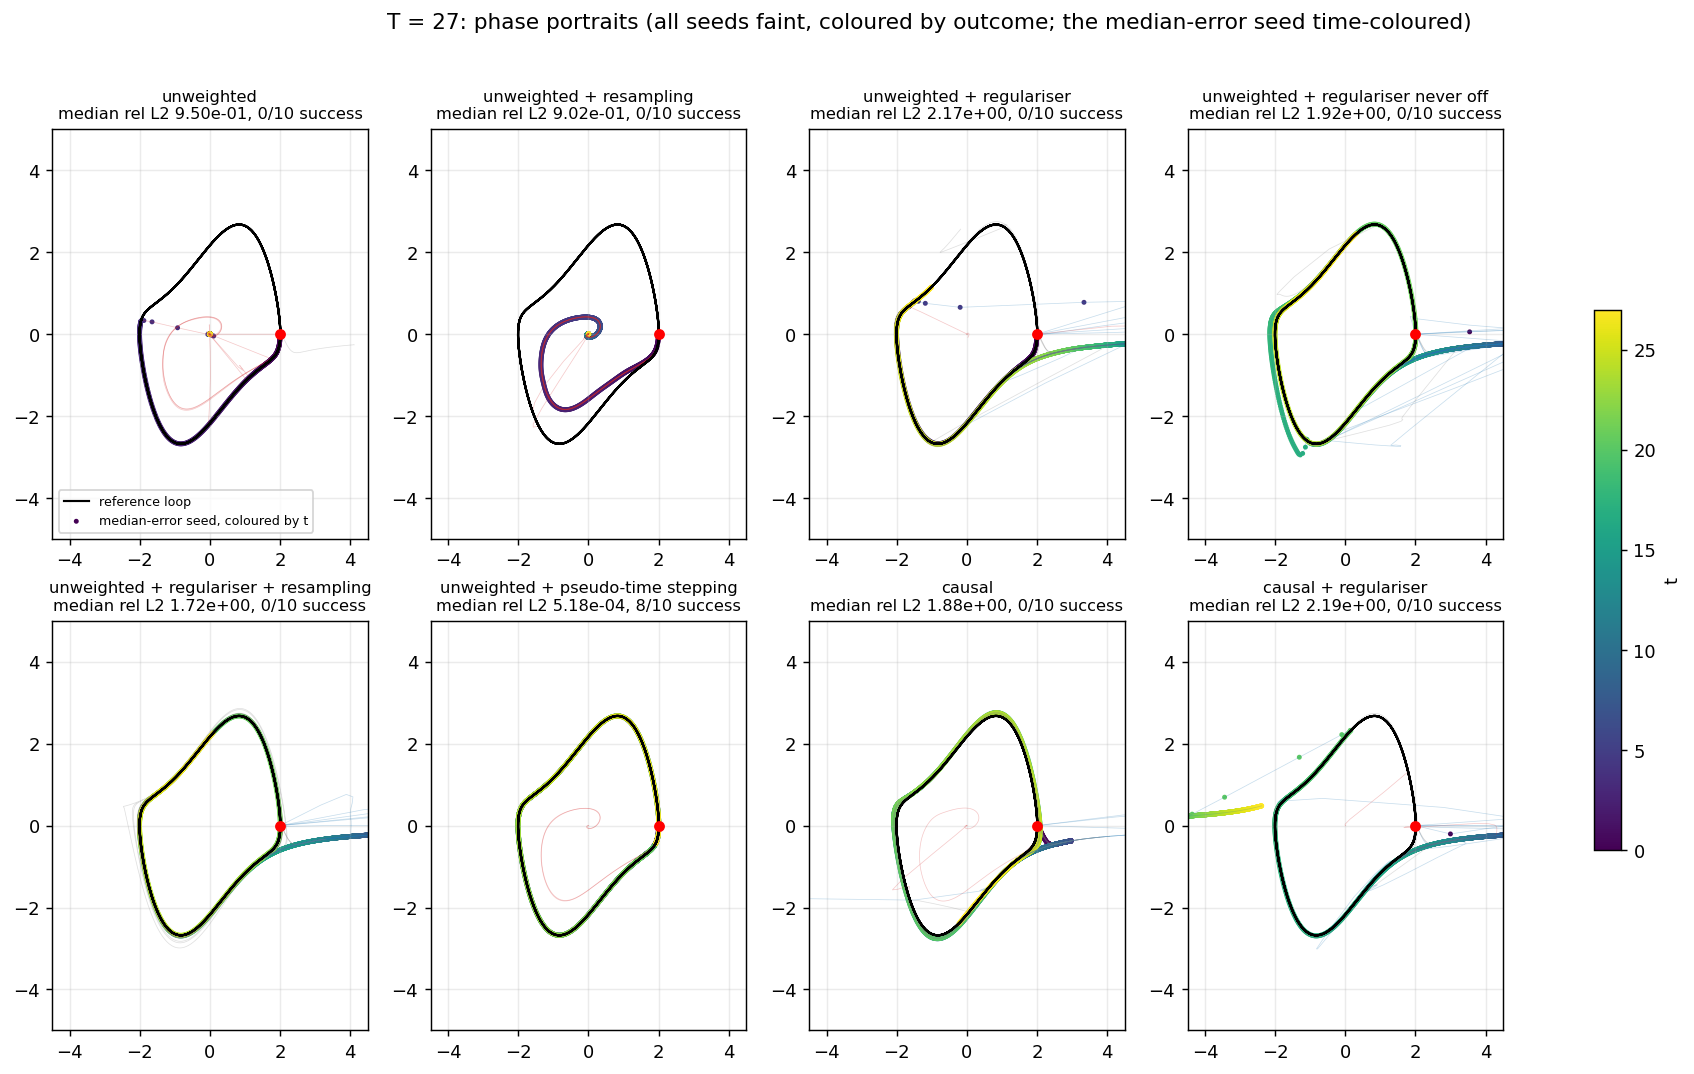
\includegraphics[width=\linewidth]{vdp_arms_phase_T27.png}
      \srcnote{Four periods, phase plane, median-error seed coloured by time.
        Plain and resampled spiral into the origin. Every regulariser variant
        enters from $y_1 \approx 4.5$, far outside the cycle, and joins the loop
        out of phase. Pseudo-time stepping draws the loop itself.}
    \end{column}
    \begin{column}{0.48\textwidth}
      \begin{itemize}\small
        \item \hl{Parked} (plain, resampled). Follows the reference for about
              one period, then sits at the origin. On a fixed set the parks
              reach the \emph{same loss as a success}. Under resampling they sit
              at loss $0.02$ to $0.03$ with zero gradient, which is exactly the
              stationary point at the layer scale that the $1/T$ formula
              predicts.
        \item \hl{Flow-following} (every regulariser variant). Satisfies the
              anchor, splices within the first unsampled gap onto a trajectory
              entering from $y_1 \approx 4.5$, and rides it onto the loop out of
              phase, at a converged loss of $10^{-5}$ to $10^{-4}$.
        \item \hl{Diffuse}, otherwise.
      \end{itemize}
      \smallskip
      \fbox{\parbox{0.93\textwidth}{\small
        Two facts from the loss-term curves. In the regularised arms the raw
        regulariser value \emph{rises} after switch-off while the objective
        keeps falling. And the polish drives the flow-following objectives below
        $10^{-4}$ \bad{without moving the error at all}. Loss and error decouple
        on that branch. That is the silent failure of the first result slide, in
        its fully converged form.}}
    \end{column}
  \end{columns}
\end{frame}

% ---- 30b: the eight arms in pictures (added 2026-09-06) -------------------
\begin{frame}[shrink=25]{The eight arms in pictures: the headline, the trajectories, and where the residual is paid}
  \vspace{1mm}
  \begin{columns}[T]
    \begin{column}{0.36\textwidth}
      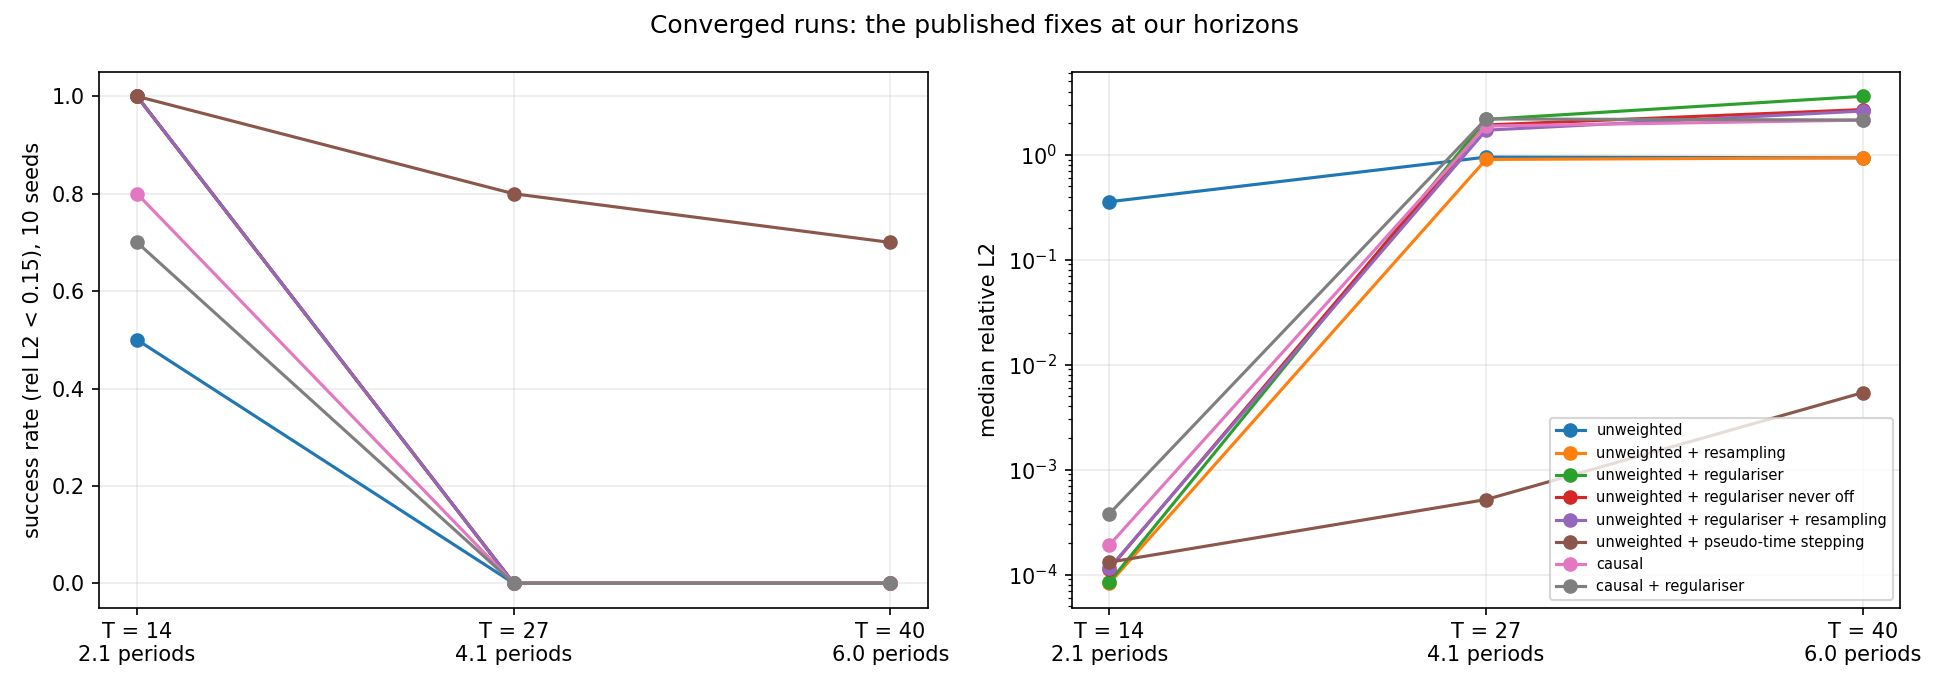
\includegraphics[width=\linewidth]{vdp_arms_summary.png}\\[1mm]
      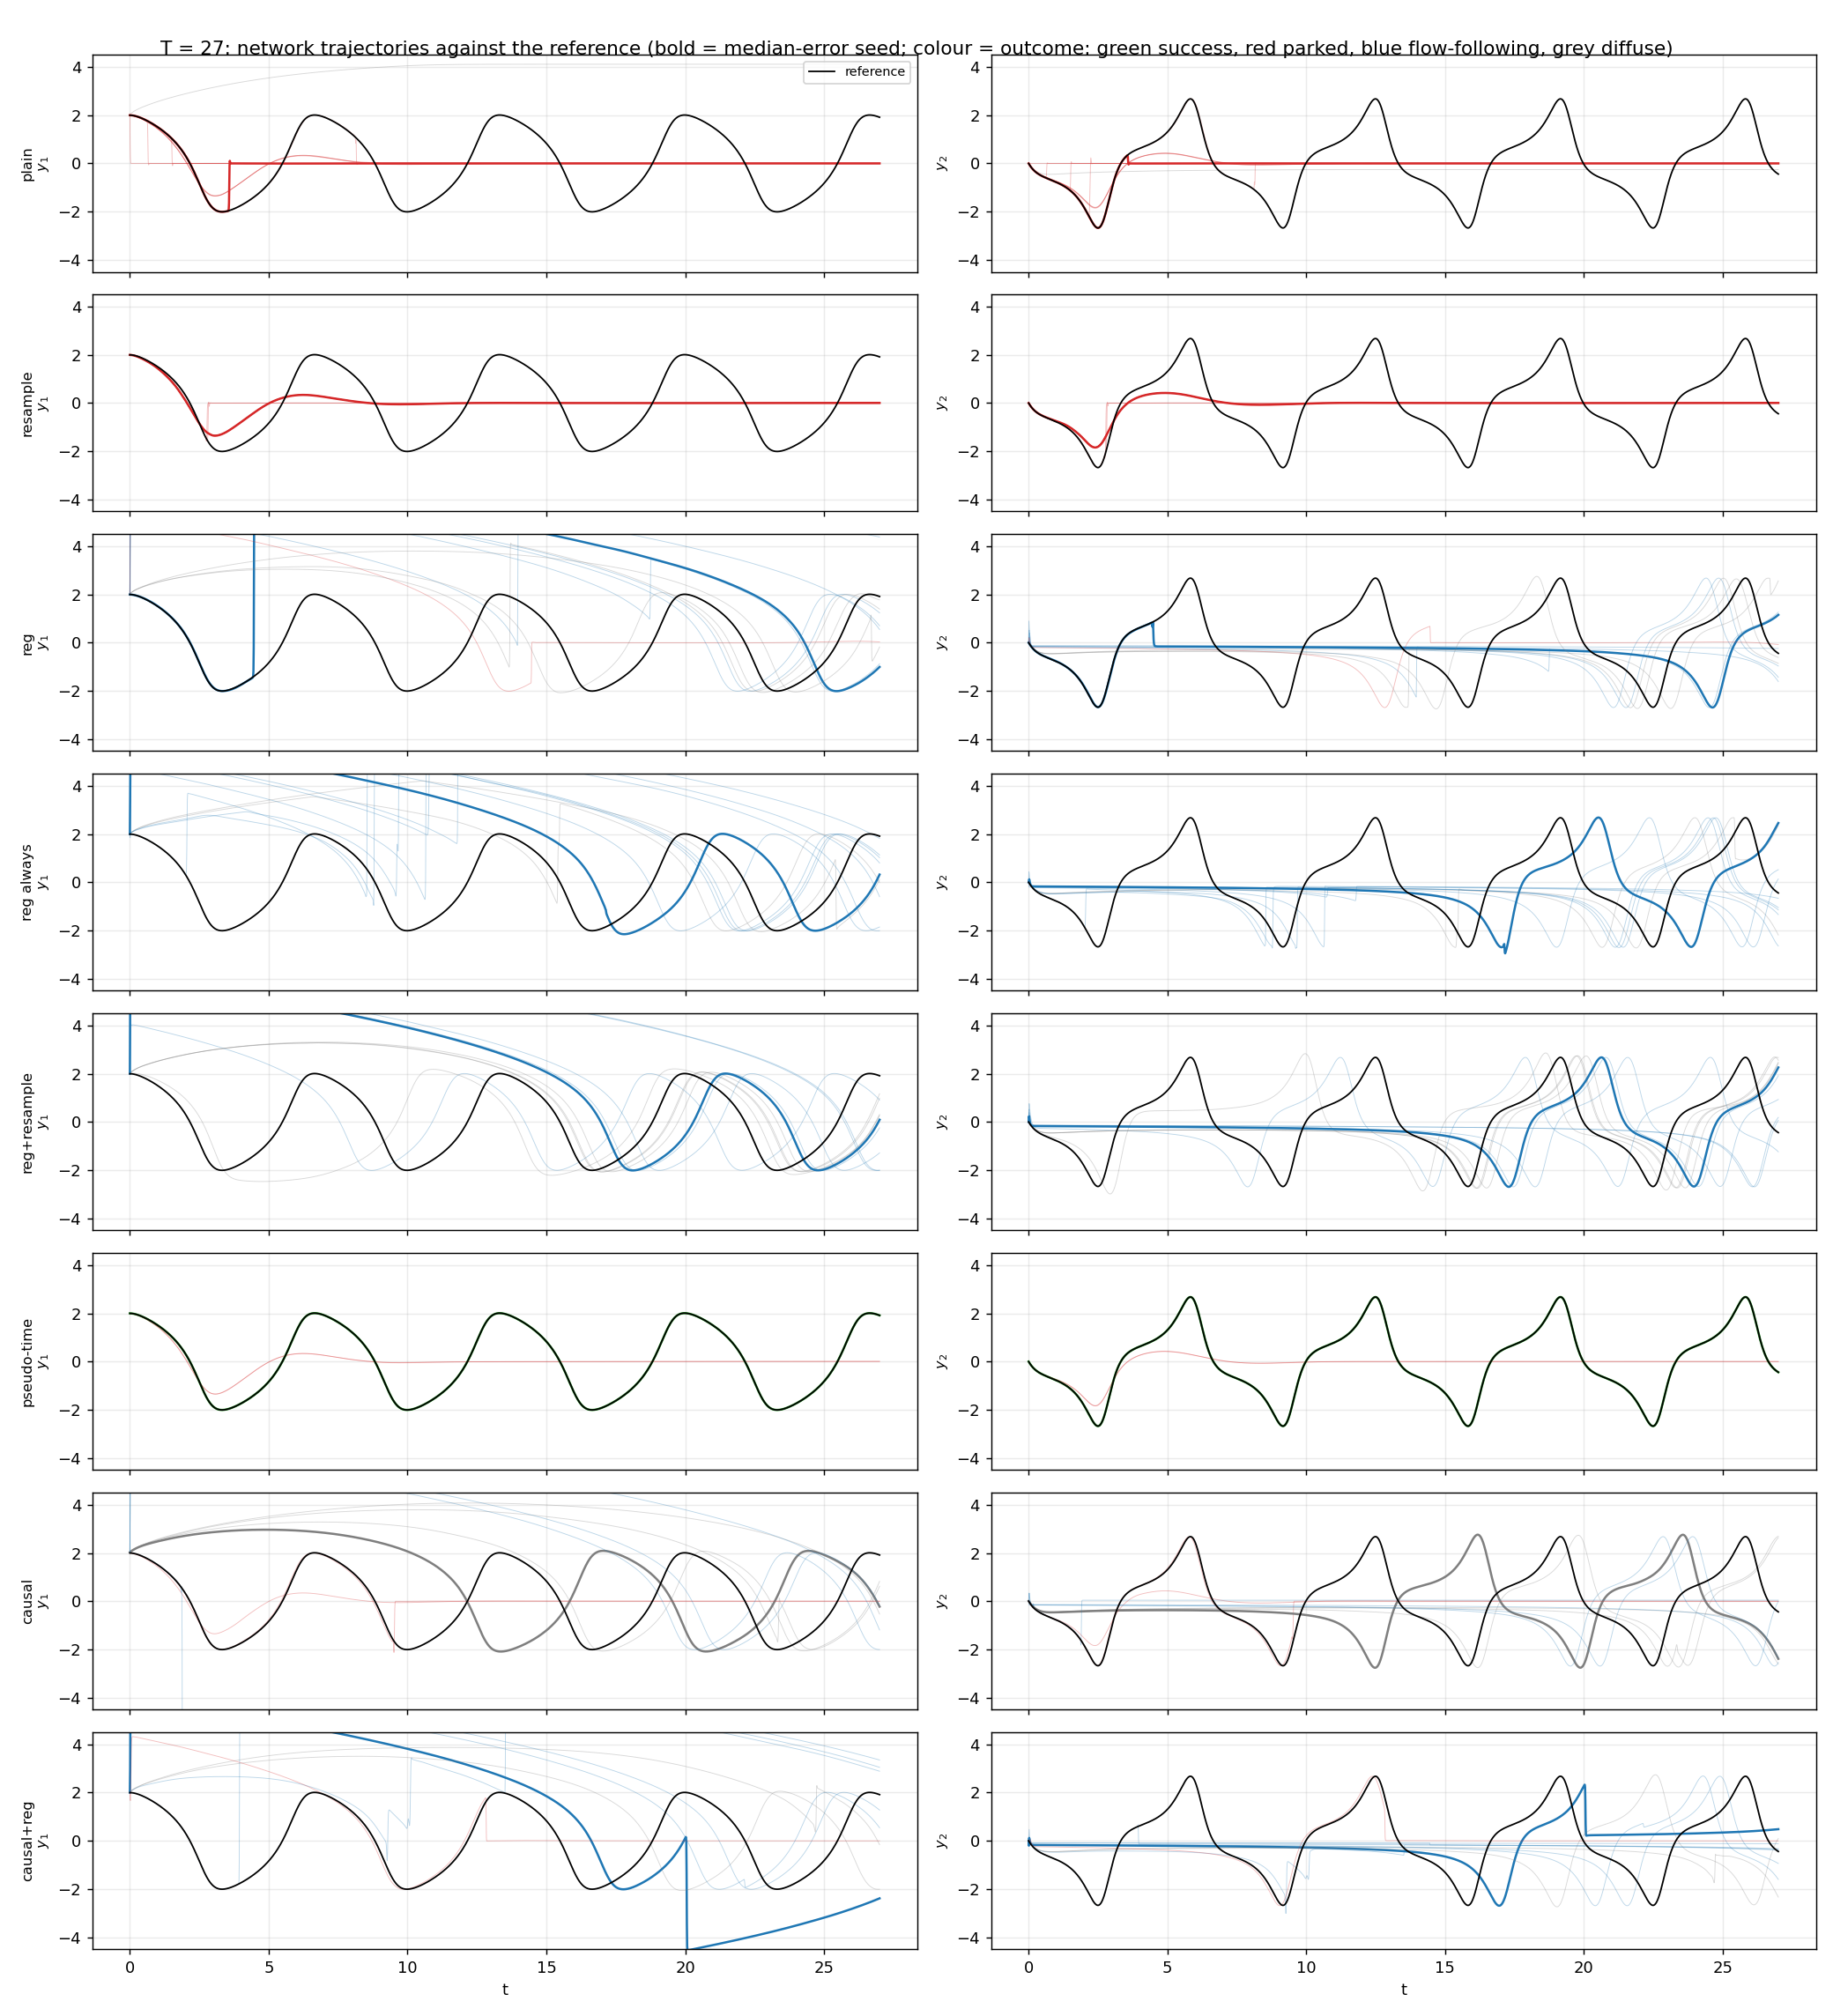
\includegraphics[width=\linewidth]{vdp_arms_traj_T27.png}
      \srcnote{Top: success rate and median error per arm and horizon. Bottom:
        four periods, both state components against time, every seed, coloured
        by outcome; the regulariser variants leave the frame at $t = 0$.}
    \end{column}
    \begin{column}{0.62\textwidth}
      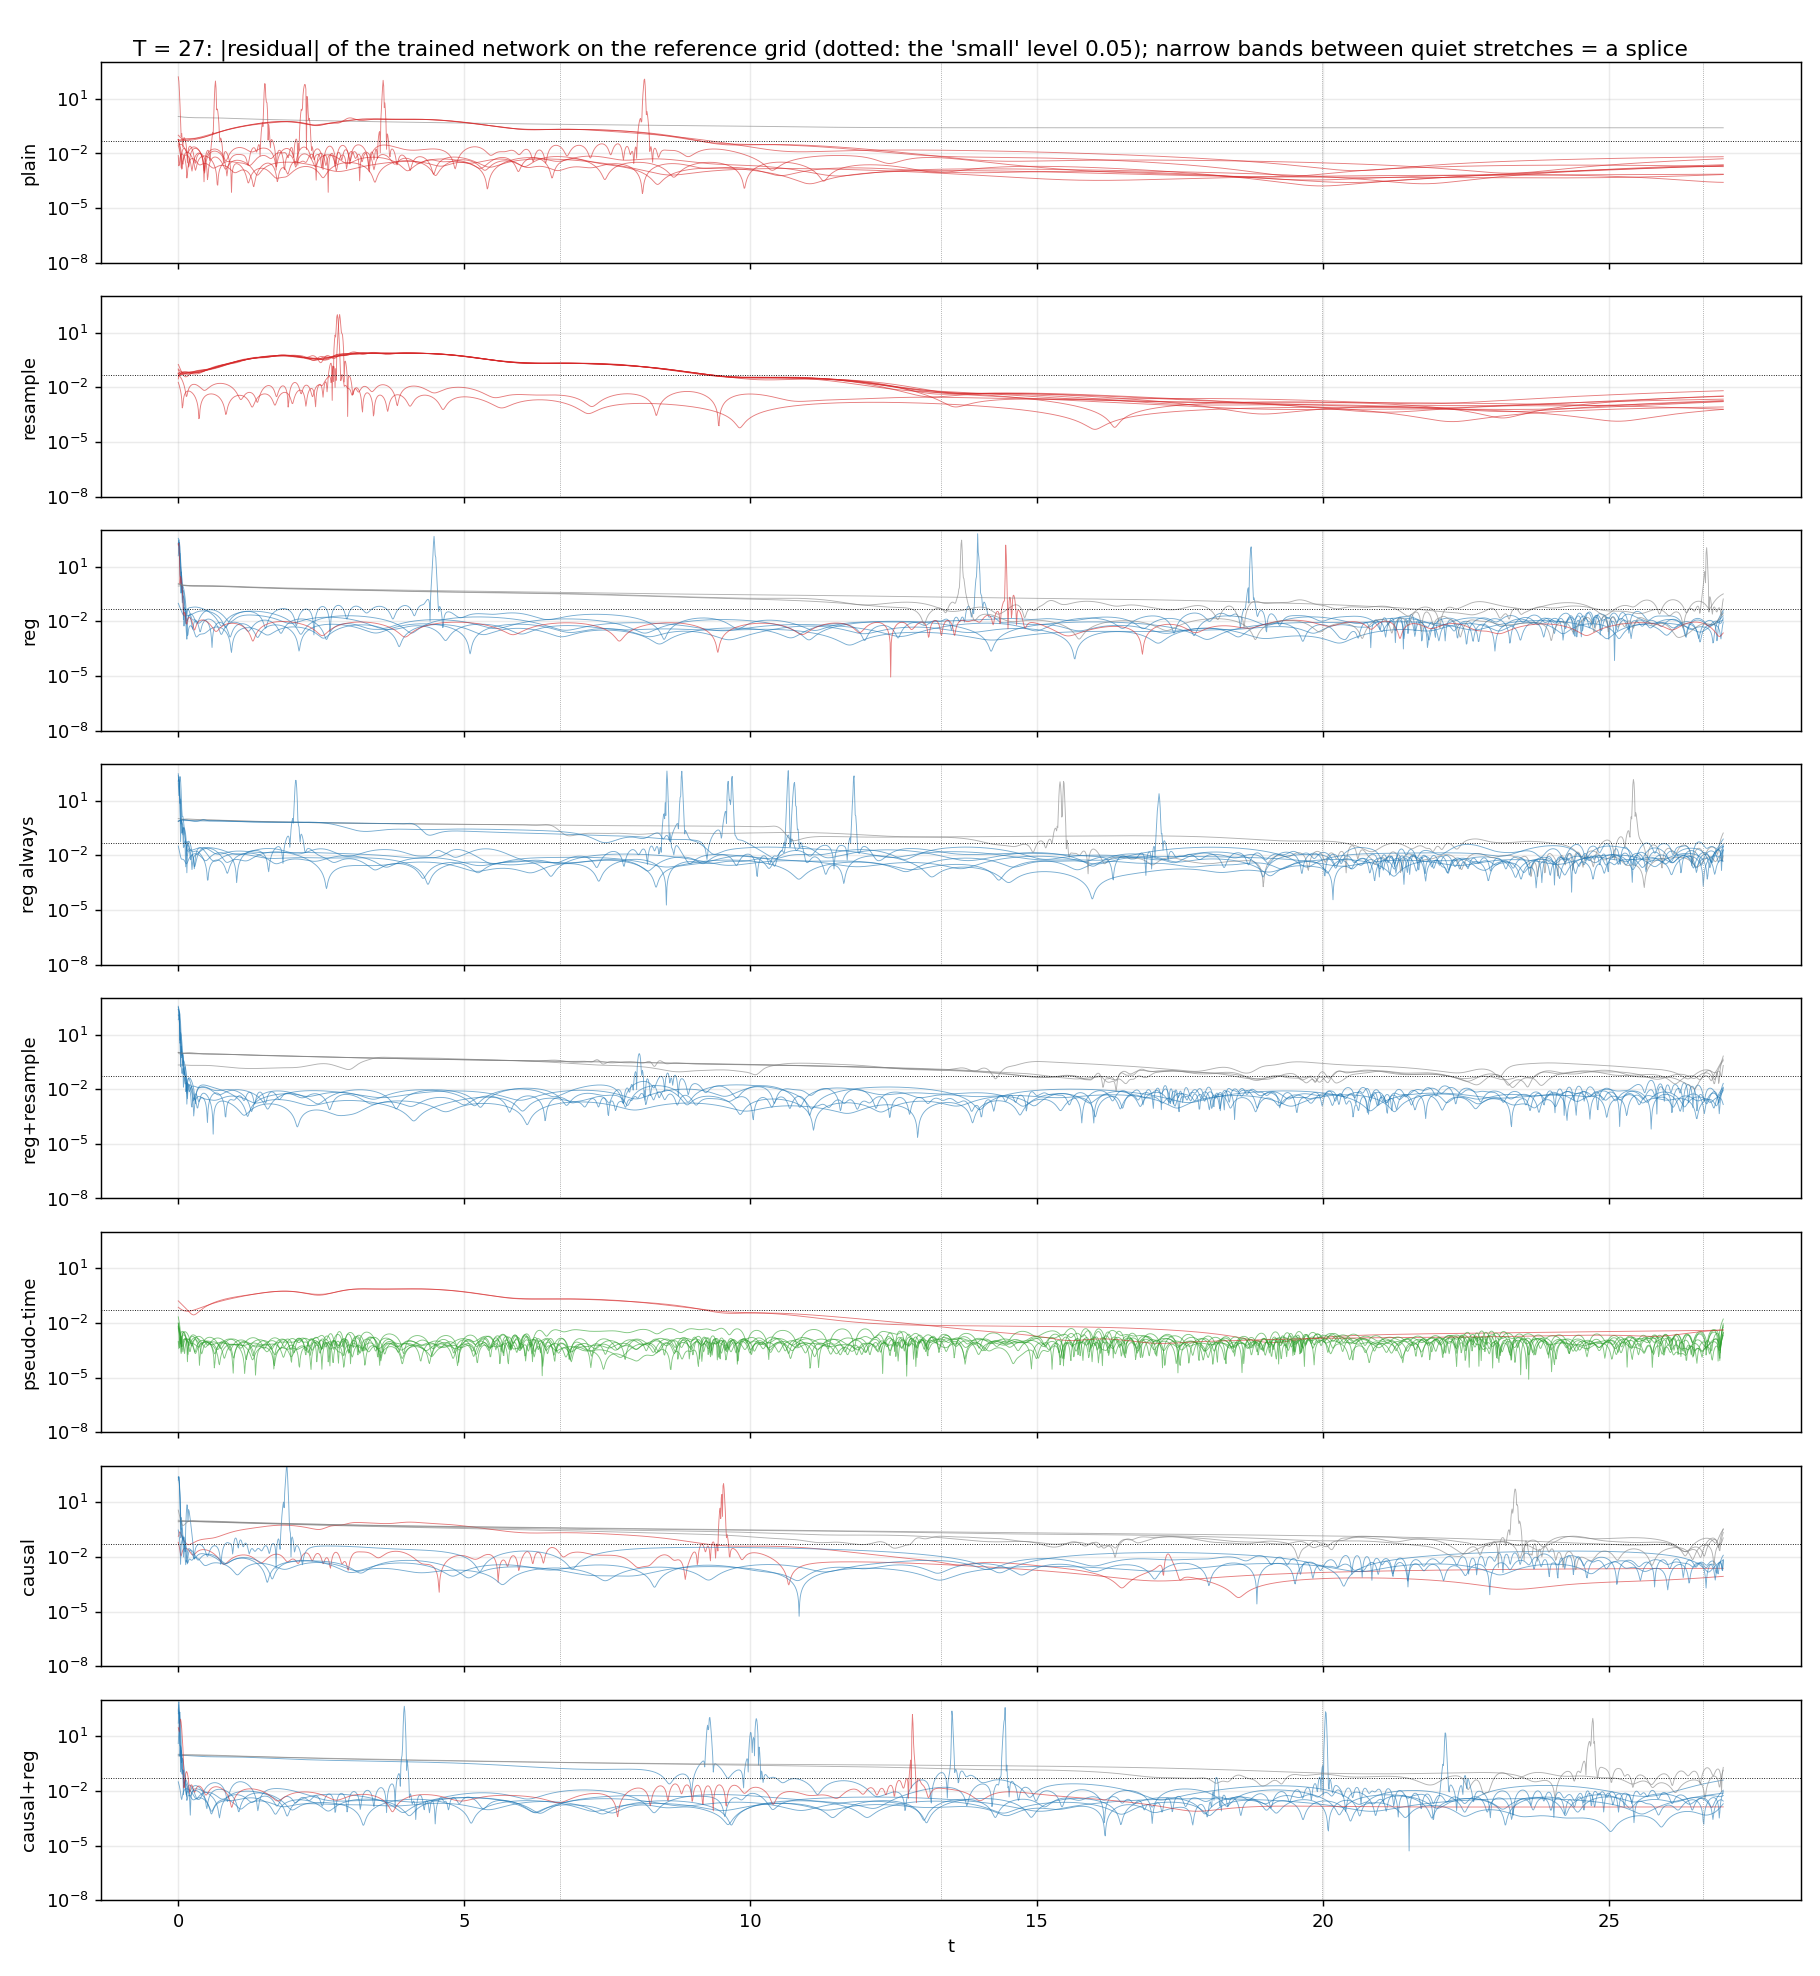
\includegraphics[width=\linewidth]{vdp_arms_residual_T27.png}
      \srcnote{The absolute residual of every trained network on the reference
        grid at four periods, dotted line at $0.05$. Parks: a moderate residual
        across the hand-over, then quiet. Every regulariser variant: below
        $0.05$ on more than $95\%$ of the window and \bad{one spike of $10^2$
        to $10^3$ immediately after $t = 0$}, the splice placed in the first
        unsampled gap. Pseudo-time successes: flat near $10^{-3}$. This panel
        is the direct evidence for the splice family; the classification of
        the previous slide is read off it.}
    \end{column}
  \end{columns}
\end{frame}

% ---- 31 ------------------------------------------------------------------
\begin{frame}[shrink=25]{The two resource axes: density buys seeds at four periods and nothing at six}
  \vspace{2mm}
  \centering\small
  \begin{tabular}{@{}lccc@{\hskip 3em}ccccc@{}}
    \toprule
    & \multicolumn{3}{c}{collocation density, $T = 27$ / $T = 40$}
    & \multicolumn{5}{c}{horizon $T$, at density 20} \\
    \cmidrule(lr){2-4}\cmidrule(lr){5-9}
    arm & 20 & 80 & 320 & 14 & 27 & 40 & 67 & 100 \\
    \midrule
    pseudo-time stepping & 8 / 7 & 9 / 5 & 10 / 8 & 10 & 8 & 7 & \bad{1} & \bad{0} \\
    plain & 0 / 0 & 0 / 0 & 0 / 0 & 5 & 0 & 0 & 0 & 0 \\
    regulariser + resampling & 0 / 0 & 3 / 0 & 0 / 0 & 10 & 0 & 0 & 0 & 0 \\
    \bottomrule
  \end{tabular}
  \vspace{1mm}

  {\scriptsize Successes out of ten. $240$ runs, ten seeds per cell, same
   protocol as the eight-arm table. Horizons $67$ and $100$ are ten and fifteen
   periods.}
  \vspace{3mm}

  \begin{columns}[T]
    \begin{column}{0.48\textwidth}
      {\small
      \begin{itemize}\small
        \item At two periods, density $80$ lifts the plain objective from $5$ of
              $10$ to $10$ of $10$, so \hl{an earlier null verdict on density,
              obtained at fixed budget with L-BFGS alone, does not survive
              training to convergence.} At four periods and beyond it still
              fails at every density, so that verdict stands.
        \item The published regulariser protocol has its first successes past two
              periods at density $80$: $3$ of $10$ at four periods, one
              converged and two budget-limited. At density $320$ it is back to
              $0$ of $10$.
      \end{itemize}}
    \end{column}
    \begin{column}{0.48\textwidth}
      {\small
      \begin{itemize}\small
        \item Pseudo-time stepping's parking rate at four periods falls with
              density, $8$, $9$, $10$. At six periods it does not move in any
              direction, $7$, $5$, $8$, with different seeds parking at each
              density and every parked run at the same loss whatever the
              density. \hl{Ten seeds cannot separate the six-period rates.}
        \item Cost grows roughly linearly with the number of points: the
              density-$320$ runs at $T = 40$, with $12{,}800$ points, took about
              four hours each.
      \end{itemize}}
    \end{column}
  \end{columns}
\end{frame}

% ---- 31b -----------------------------------------------------------------
\begin{frame}[shrink=25]{The two axes as pictures: a rate that moves with density, and a wall that does not}
  \vspace{1mm}
  \begin{columns}[T]
    \begin{column}{0.34\textwidth}
      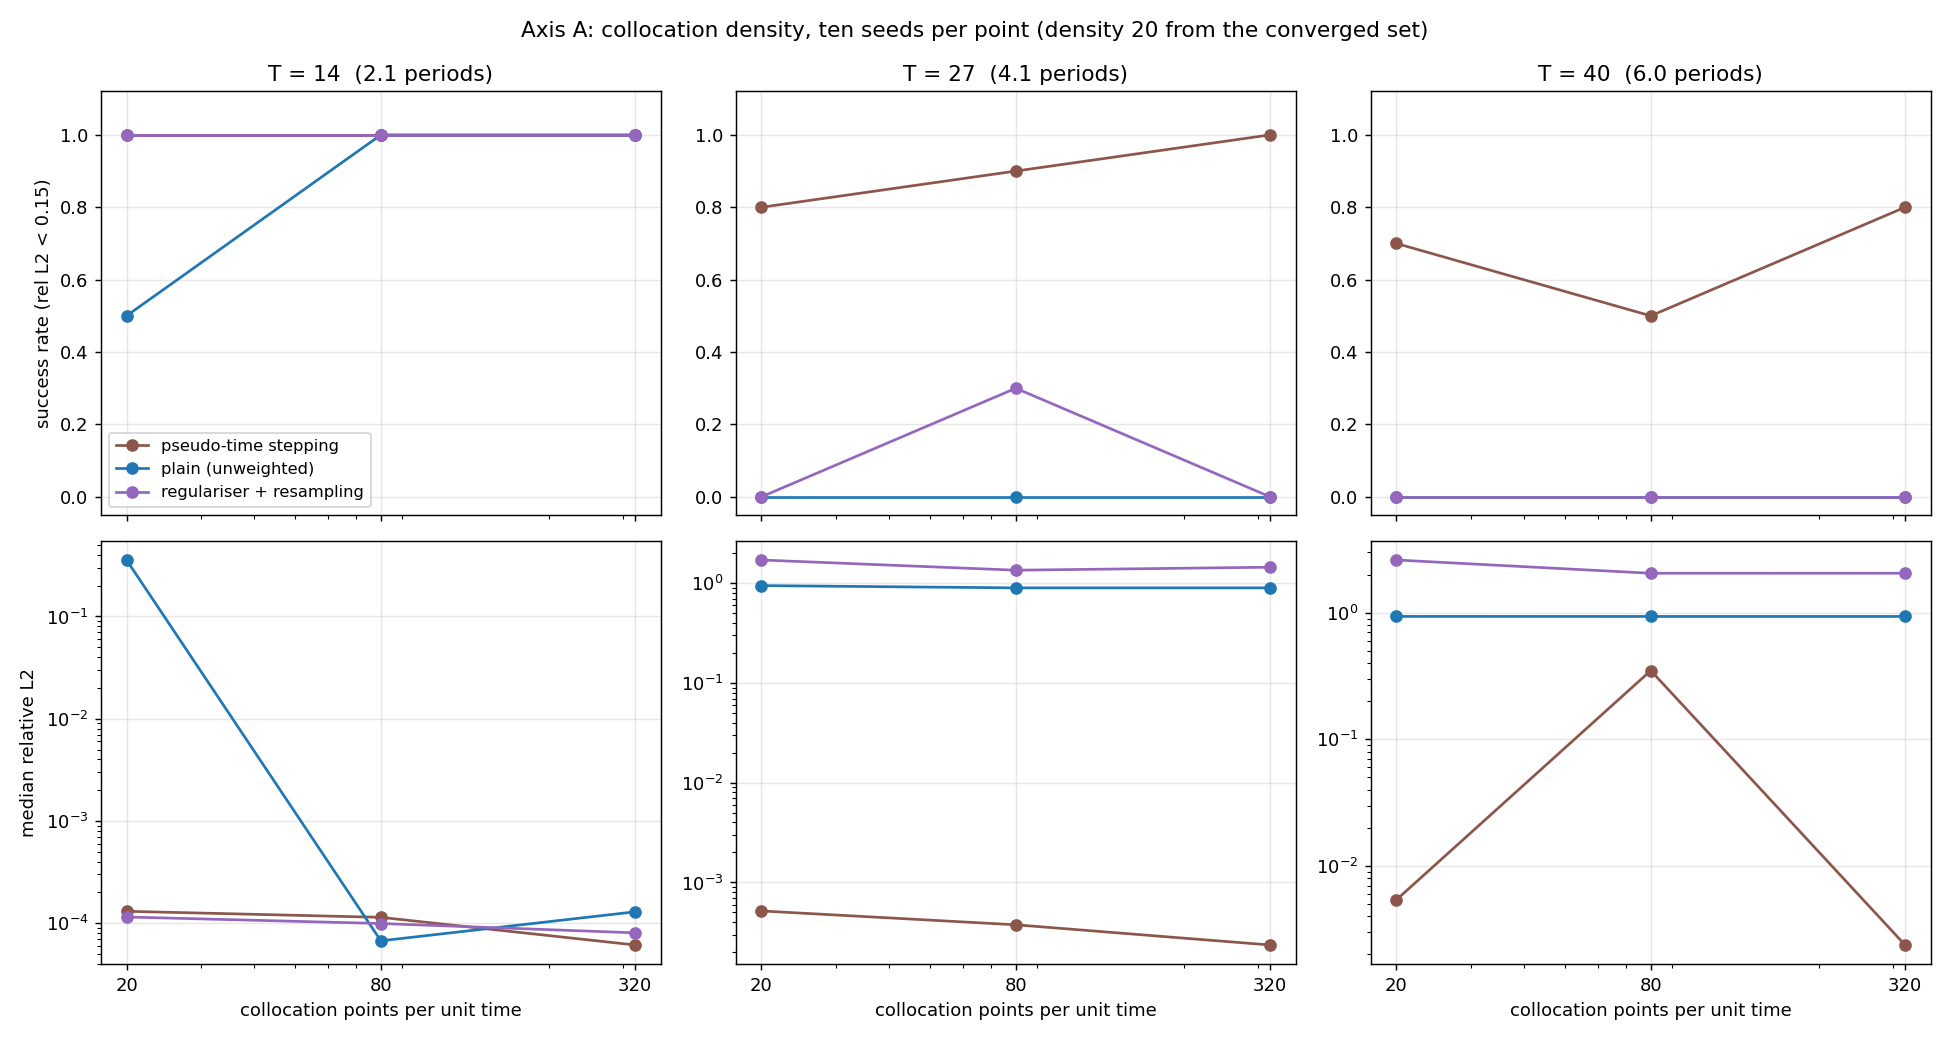
\includegraphics[width=\linewidth]{vdp_axes_density.png}
      \srcnote{Success rate (top) and median relative $L_2$ (bottom) against
        collocation density, one column per horizon, ten seeds per point.}
    \end{column}
    \begin{column}{0.34\textwidth}
      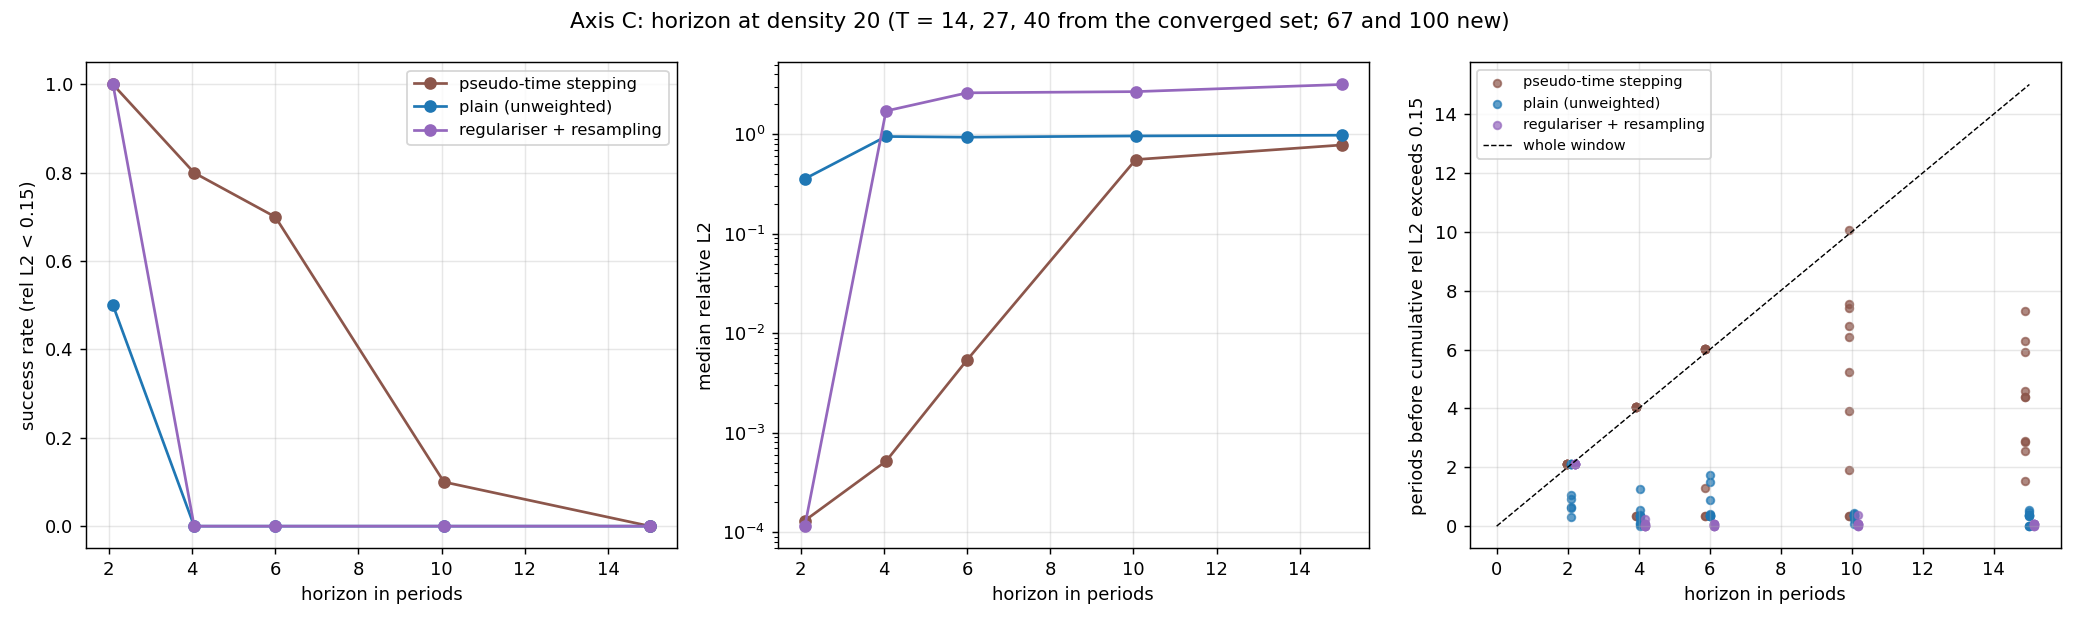
\includegraphics[width=\linewidth]{vdp_axes_horizon.png}
      \srcnote{Success, median relative $L_2$, and the number of periods
        survived before the cumulative relative $L_2$ exceeds $0.15$, per run,
        against the horizon in periods.}
    \end{column}
    \begin{column}{0.30\textwidth}
      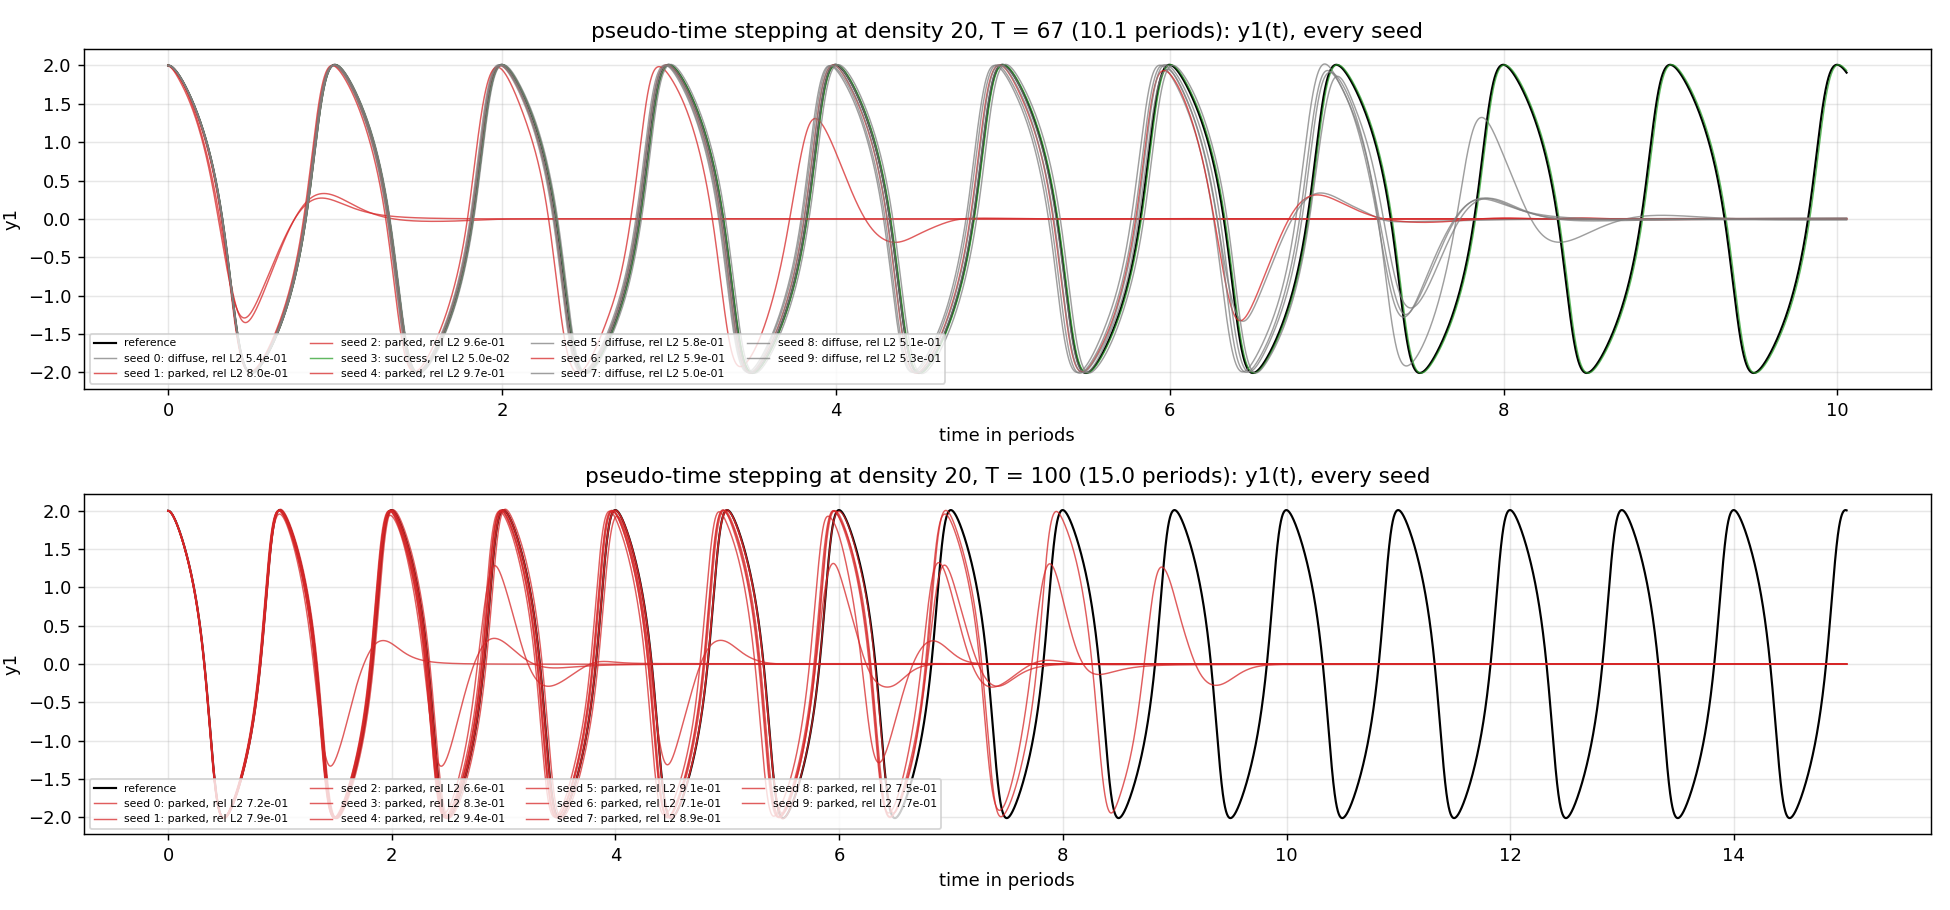
\includegraphics[width=\linewidth]{vdp_axes_long_horizon.png}
      \srcnote{Pseudo-time stepping at ten and fifteen periods, $y_1$ against
        time in periods for every seed, coloured by class.}
      \vspace{-2mm}
      {\small \hl{The failures at long horizon are late parks}: the network
       rides the loop for four to eight periods, drifts off, and sits at the
       origin. \bad{Nothing wanders off the loop.} The failure mode does not
       change with the horizon, it arrives later.
       \smallskip

       One consequence for reporting: the classifier reads a late park as
       diffuse, so the periods-survived panel is the right readout for long
       windows, not the success rate.}
    \end{column}
  \end{columns}
\end{frame}

% ---- 32 ------------------------------------------------------------------
\begin{frame}[shrink=25]{The \texorpdfstring{$1/T$}{1/T} price is not a story, it is a measured line}
  \vspace{1mm}
  \begin{columns}[T]
    \begin{column}{0.48\textwidth}
      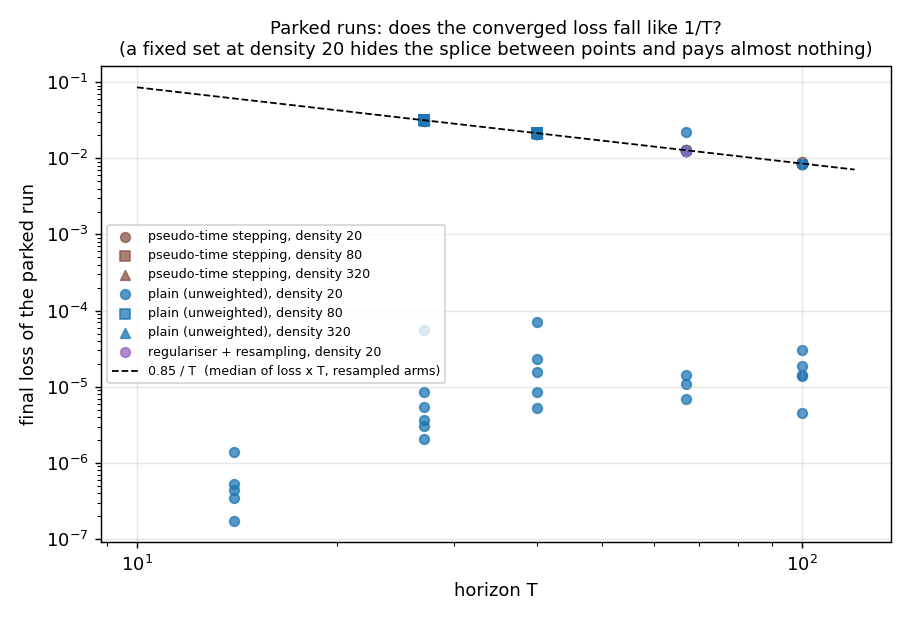
\includegraphics[width=0.92\linewidth]{vdp_axes_parked_loss.png}
      \srcnote{The converged loss of every parked run against $T$, with the
        $1/T$ line drawn through the median of loss $\times\ T$ over the
        resampled arms.}
    \end{column}
    \begin{column}{0.5\textwidth}
      \begin{itemize}\small
        \item Over the \hl{$65$ parked runs whose transition layer is actually
              sampled} (the resampled arms at any density, and the plain arm at
              densities $80$ and $320$), \hl{loss $\times\ T$ has median $0.85$
              and ranges $0.84$ to $0.90$}, from $T = 27$ to $T = 100$.
        \item The plain arm's parked runs at density $20$ sit three to four
              orders of magnitude lower, because a fixed set of $20$ points per
              unit time leaves room to hide the layer. At density $80$ the gap
              is too small to hide in, and a fixed set behaves like resampling.
        \item \hl{Two consequences.} The $1/T$ prediction holds quantitatively.
              And \bad{more density cannot move a resampled method's wall by
              pricing}, because the parked branch is already fully sampled, so
              denser points do not raise its price. What density can do is make
              the descent to the truth cheaper than the descent to the park in
              more seeds, which is what the four-period column shows and the
              six-period column does not.
      \end{itemize}
      \smallskip
      {\small The wall between six and ten periods is a \emph{late} park: the
       network rides the loop for four to eight periods, drifts off, and sits at
       the origin. Nothing wanders off the loop. What sets its position is not
       yet measured.}
    \end{column}
  \end{columns}
\end{frame}

% ---- 33 ------------------------------------------------------------------
\begin{frame}[shrink=25]{The discrete-time column has no such failure, and its floor is not the scheme}
  \vspace{1mm}
  \begin{columns}[T]
    \begin{column}{0.46\textwidth}
      \centering\small
      \begin{tabular}{@{}ccc@{}}
        \toprule
        $q$ (order $2q$) & trained network & exact scheme \\
        \midrule
        2 (4)   & $3.94\times10^{-2}$ & $4.20\times10^{-2}$ \\
        4 (8)   & $4.57\times10^{-3}$ & $2.20\times10^{-4}$ \\
        8 (16)  & $3.61\times10^{-3}$ & $2.38\times10^{-8}$ \\
        16 (32) & $3.63\times10^{-3}$ & $8.9\times10^{-14}$ \\
        32 (64) & $3.63\times10^{-3}$ & $1.4\times10^{-13}$ \\
        \bottomrule
      \end{tabular}
      \smallskip

      {\scriptsize Endpoint relative $L_2$ on the $441$ held-out states, median
       over three seeds, against the exactly solved scheme on the same states
       and metric. Step $\Delta t = 0.8$.}
      \smallskip

      {\small Capped measure, same runs: median $\rho$ falls $7.2\times10^{-5}$,
       $1.0\times10^{-5}$, $6.5\times10^{-6}$, $6.0\times10^{-6}$,
       $5.1\times10^{-6}$. And $\sqrt{6.5\times10^{-6}} \approx 2.5\times10^{-3}$,
       consistent with the relative $L_2$ floor as it must be.}
    \end{column}
    \begin{column}{0.52\textwidth}
      \begin{itemize}\small
        \item All fifteen runs converge to losses of $7\times10^{-6}$ to
              $2.6\times10^{-5}$, with no collapse and no divergence. And,
              unlike every failed continuous-time run, \hl{the loss is an honest
              proxy for the error}: a squared-residual loss of $10^{-5}$
              resolves outputs to roughly its square root, which is where the
              held-out error lands.
        \item At $q = 2$ the network sits \emph{on} the exactly solved scheme's
              own error: the map is scheme-limited, and even a perfect fit would
              be that wrong.
        \item From $q = 4$ the curves part. The scheme drops ten orders of
              magnitude to roundoff; the network stays flat at
              \hl{$3.6$ to $4.6\times10^{-3}$}, within a factor $1.27$ for all
              $q \ge 4$, all seeds agreeing.
        \item Asking for $66$ outputs at $q = 32$ instead of $18$ at $q = 8$
              degrades nothing, and the largest errors sit at the corners of the
              training region where the dynamics are fastest.
        \item So all later work fixes $q = 8$: the scheme's own error is five
              orders below the network's, and nothing about the network is
              masked by the scheme.
      \end{itemize}
    \end{column}
  \end{columns}
\end{frame}

% ---- 33b -----------------------------------------------------------------
\begin{frame}[shrink=25]{The same floor twice: against stages, and across forty-five architectures}
  \vspace{1mm}
  \begin{columns}[T]
    \begin{column}{0.42\textwidth}
      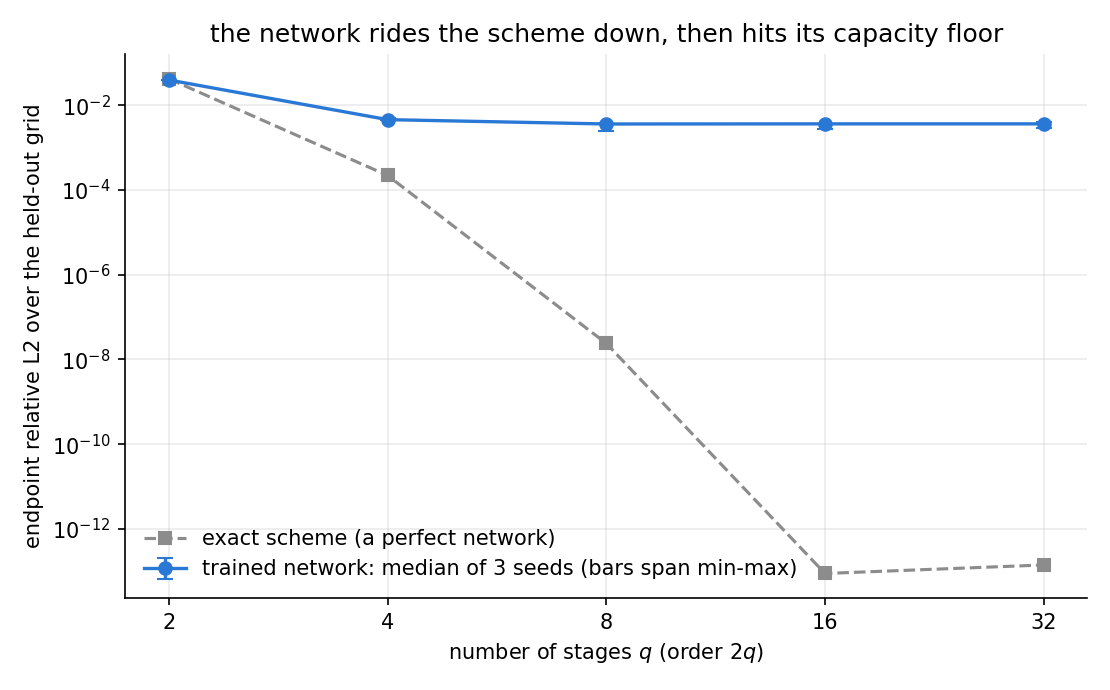
\includegraphics[width=\linewidth]{vdp_capacity_floor.png}
      \srcnote{Endpoint relative $L_2$ against the number of stages: the trained
        network (median of three seeds, min to max whiskers) rides the scheme's
        error down and then flattens onto its own floor, while the exactly
        solved scheme continues to machine precision.}
    \end{column}
    \begin{column}{0.56\textwidth}
      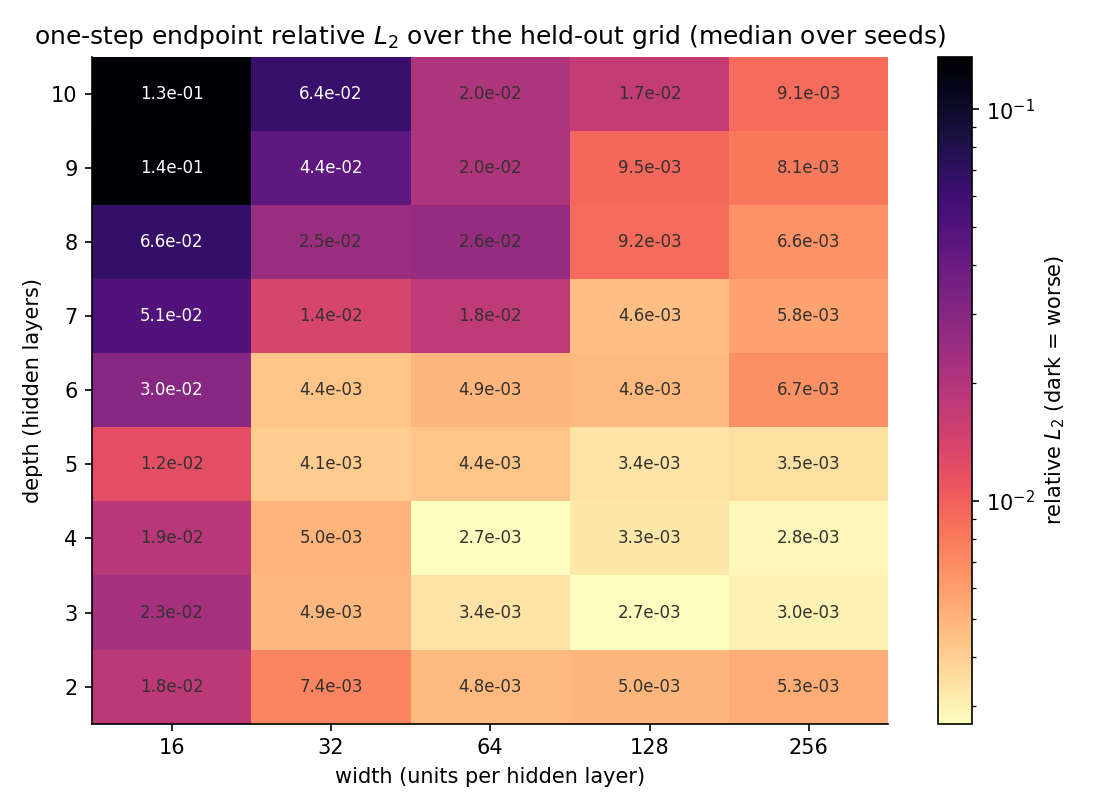
\includegraphics[width=\linewidth]{vdp_size_map_discrete.png}
      \srcnote{One-step error over the architecture grid at fixed $q = 8$:
        depth $\times$ width, three seeds each. No entry approaches the exactly
        solved scheme; depth harms beyond about five layers, width stops helping
        beyond $64$ to $128$ units, and the worst corner sits at
        $1.3\times10^{-1}$.}
      \vspace{-2mm}
      {\small Two pictures, one statement. \hl{More stages cannot help} once the
       scheme's error is below the network's, and \hl{more parameters cannot
       help either}, because the binding constraint in both cases is how far the
       optimiser got. That is the finding the LHCb architecture grid then
       reproduced independently, on a five-component non-autonomous system with
       a measured field.}
    \end{column}
  \end{columns}
\end{frame}

% ---- 34 ------------------------------------------------------------------
\begin{frame}[shrink=25]{On van der Pol the floor is the optimiser, and the horizon is decided by the seed}
  \vspace{1mm}
  \begin{columns}[T]
    \begin{column}{0.46\textwidth}
      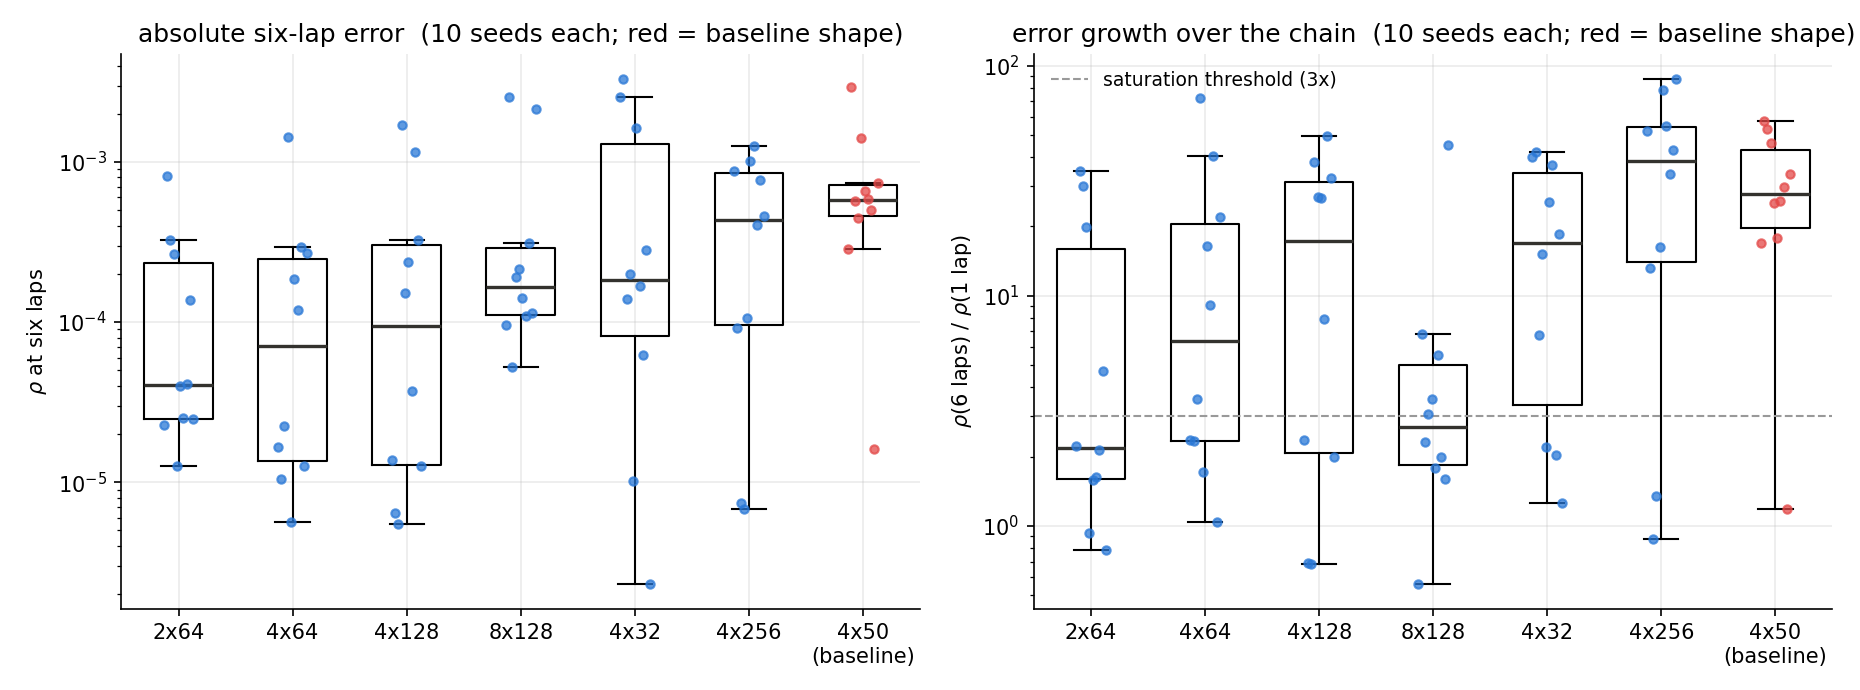
\includegraphics[width=\linewidth]{vdp_seed_replication.png}
      \srcnote{Ten seeds for each of seven architectures, six-period chained
        error. The seed-to-seed spread within one architecture rivals the whole
        grid's spread.}
    \end{column}
    \begin{column}{0.52\textwidth}
      \textbf{Design.} Depth $\{2,\dots,10\}$ crossed with width
      $\{16, 32, 64, 128, 256\}$, $45$ architectures at $q = 8$, three seeds,
      $135$ runs, everything else frozen. Seven architectures then at ten seeds.
      The $108$ test starts are split: $50$ used only to rank, $58$ held out and
      used only to report.
      \begin{itemize}\small
        \item \hl{The floor does not move.} Best of $45$ is $2.5\times10^{-3}$,
              a factor $1.5$ below the $4\times50$ configuration, and still five
              orders above the exact scheme. Depth beyond about $5$ hurts
              sharply; width stops helping beyond $64$ to $128$.
        \item \hl{The binding constraint is the optimiser.} Spearman rank
              correlation between converged training loss and held-out one-step
              error over the $135$-run grid: \hl{$+0.974$}. Architectures that
              fail also fail to train. No capacity-rich, badly-generalising
              regime exists.
        \item \hl{But that same loss ranks six-period chained error at only
              $+0.35$.} Long horizons are decided by the seed: the growth ratio
              varies $13\times$ between seeds of one architecture and
              $300\times$ across the grid.
      \end{itemize}
    \end{column}
  \end{columns}
\end{frame}

% ---- 35 ------------------------------------------------------------------
\begin{frame}[shrink=25]{Growth is a measurable, transferable property, so select the seed on the chain}
  \vspace{1mm}
  \begin{columns}[T]
    \begin{column}{0.5\textwidth}
      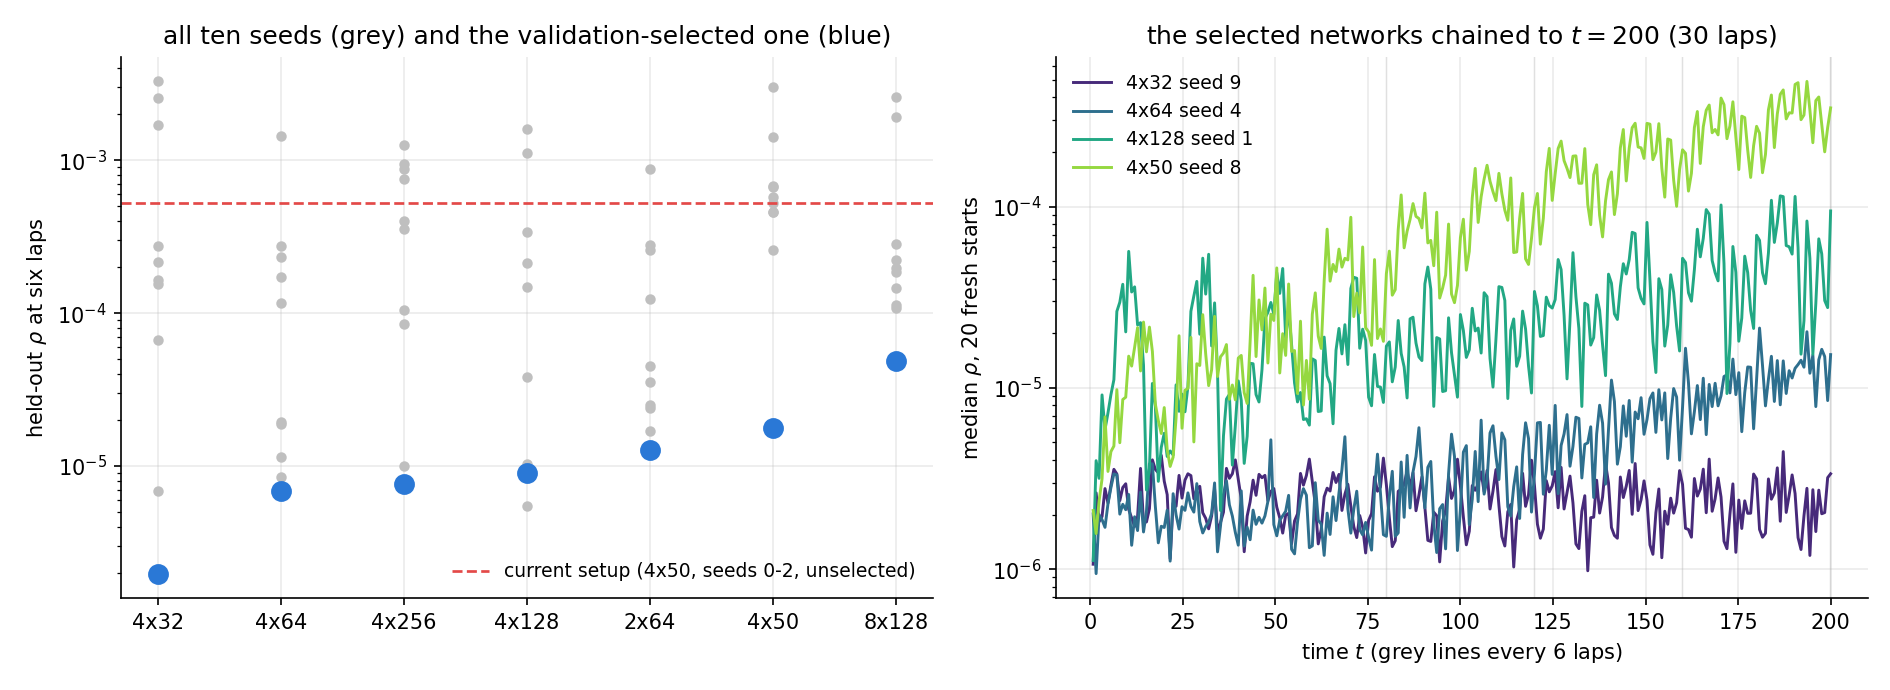
\includegraphics[width=\linewidth]{vdp_selection.png}
      \srcnote{The selection payoff and the far-horizon check:
        validation-selected networks against their unselected siblings, and the
        selected network holding $\rho \approx 3\times10^{-6}$ flat to thirty
        periods on fresh starts.}
    \end{column}
    \begin{column}{0.48\textwidth}
      \begin{itemize}\small
        \item A validation chain to the target horizon predicts held-out
              six-period error at Spearman \hl{$+0.98$}; the training loss and
              the one-step error predict it at only $+0.35$, and a one-period
              chain at $+0.67$.
        \item \hl{The protocol:} train about ten seeds; chain each on the
              validation starts to the target horizon; keep the smallest.
              Selection beats the median seed by a factor $3$ to $96$.
        \item The far-horizon check separates the front-runners: chained to
              thirty periods from twenty fresh starts, the $4\times32$ choice
              moved from $3.1\times10^{-6}$ to $3.4\times10^{-6}$, a factor
              $1.1$, while the $4\times64$, $4\times128$ and $4\times50$ choices
              grew by factors $11.3$, $8.7$ and $24$.
        \item \bad{Caveat carried forward:} a six-period validation window does
              not guarantee thirty periods for every candidate. The protocol's
              window must match the horizon the map will be used at.
      \end{itemize}
      \smallskip
      {\small The reported network is the $4\times32$ seed-9 map, $3858$
       parameters.}
    \end{column}
  \end{columns}
\end{frame}

% ---- 36 ------------------------------------------------------------------
\begin{frame}[shrink=25]{Chaining beats one large step, and physics buys data-independence rather than accuracy}
  \vspace{1mm}
  \begin{columns}[T]
    \begin{column}{0.5\textwidth}
      \centering\scriptsize
      \begin{tabular}{@{}cccl@{}}
        \multicolumn{4}{c}{\textbf{whole trajectories, relative $L_2$}}\\
        \toprule
        $T$ & chained, $4{\times}50$ seeds & chained, selected $4{\times}32$ & continuous-time, plain \\
        \midrule
        3  & $2.6\times10^{-3}$ & $1.6\times10^{-3}$ & $3.8\times10^{-5}$ \\
        7  & $4.8\times10^{-3}$ & $2.1\times10^{-3}$ & $6.6\times10^{-4}$ \\
        14 & $9.0\times10^{-3}$ & $2.1\times10^{-3}$ & $0.79$ \\
        27 & $1.8\times10^{-2}$ & $2.1\times10^{-3}$ & $0.90$ \\
        40 & $2.6\times10^{-2}$ & $2.0\times10^{-3}$ & $0.94$ \\
        \bottomrule
      \end{tabular}
      \smallskip

      {\scriptsize Pooled over three seeds and $108$ test starts; single network
       for the selected column. The continuous-time column is a
       \emph{dedicated} fit to one start at $T \le 7$.}
      \smallskip

      {\small The unselected seeds compound gently, a factor $10$ over six
       periods. The selected network's column is \hl{flat}, a factor $1.3$ from
       half a period to six, and twelve times better than the best unselected
       seed at six periods. At the matched horizon, chaining beats the
       one-giant-step mode by a factor $10$.
       \smallskip

       Feasibility of the giant step was checked first with the exact solver: at
       a full period in one step the stage equations stop being reliably
       solvable even at $q = 64$. A-stability is a linear property; what binds
       is nonlinear solvability.}
    \end{column}
    \begin{column}{0.48\textwidth}
      \centering\scriptsize
      \begin{tabular}{@{}cccc@{}}
        \multicolumn{4}{c}{\textbf{physics against perfect labels, matched pair}}\\
        \toprule
        $n$ & physics & data & integrator steps for labels \\
        \midrule
        50   & $9.2\times10^{-3}$ & $9.8\times10^{-3}$ & $39{,}950$ \\
        125  & $6.3\times10^{-3}$ & $3.0\times10^{-3}$ & $99{,}875$ \\
        250  & $4.1\times10^{-3}$ & $1.8\times10^{-3}$ & $199{,}750$ \\
        500  & $3.4\times10^{-3}$ & $1.6\times10^{-3}$ & $399{,}500$ \\
        1000 & $3.4\times10^{-3}$ & $1.7\times10^{-3}$ & $799{,}000$ \\
        2000 & $3.6\times10^{-3}$ & $1.6\times10^{-3}$ & $1{,}598{,}000$ \\
        \bottomrule
      \end{tabular}
      \smallskip

      {\small Identical network, identical seeded initial weights, identical
       optimiser and budget. Only the loss and $n$ differ. Both flatten from
       $n \approx 500$, \hl{a stable factor $2.1$ apart}, with the physics
       variant ahead only at $n = 50$.
       \smallskip

       The last column is $799n$: the labels for one state are eight true stage
       states plus the endpoint, produced by running the reference across the
       step at $10^{-3}$ and halting exactly at each stage time. \hl{The physics
       variant's reference cost is exactly zero at every $n$.}
       \smallskip

       At $q = 8$ the two losses' minimisers differ by $2.4\times10^{-8}$, five
       orders below either variant's error, so the gap is not an information gap
       but a difference in the path the optimiser takes.}
    \end{column}
  \end{columns}
\end{frame}

% =========================================================================
% VI. RESULTS, LHCb
% =========================================================================

% ---- 38b: the discrete column in pictures (added 2026-09-06) --------------
\begin{frame}[shrink=25]{The discrete-time column in pictures: both formulations on one axis, the test set, and the label bill}
  \vspace{1mm}
  \begin{columns}[T]
    \begin{column}{0.33\textwidth}
      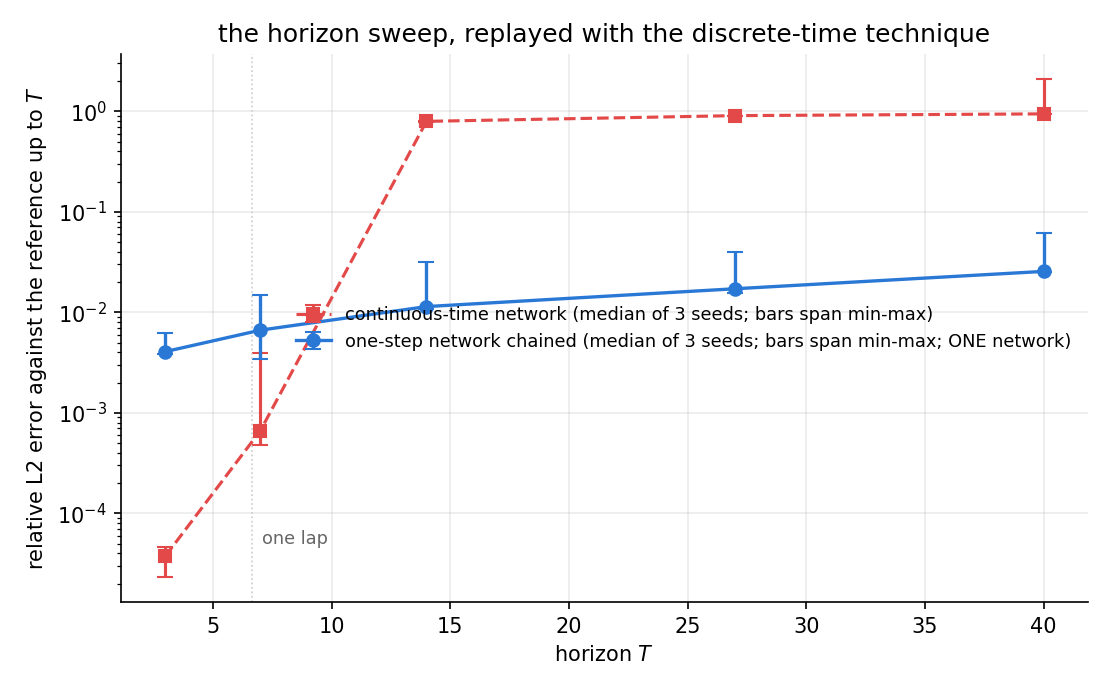
\includegraphics[width=\linewidth]{vdp_head_to_head.png}
      \srcnote{Both formulations at the continuous-time sweep's horizons. From
        four periods on no continuous-time variant produces a usable
        trajectory; the chained map's pooled median stays at $2\times10^{-3}$.
        Below one period the dedicated fits are the more accurate.}
    \end{column}
    \begin{column}{0.33\textwidth}
      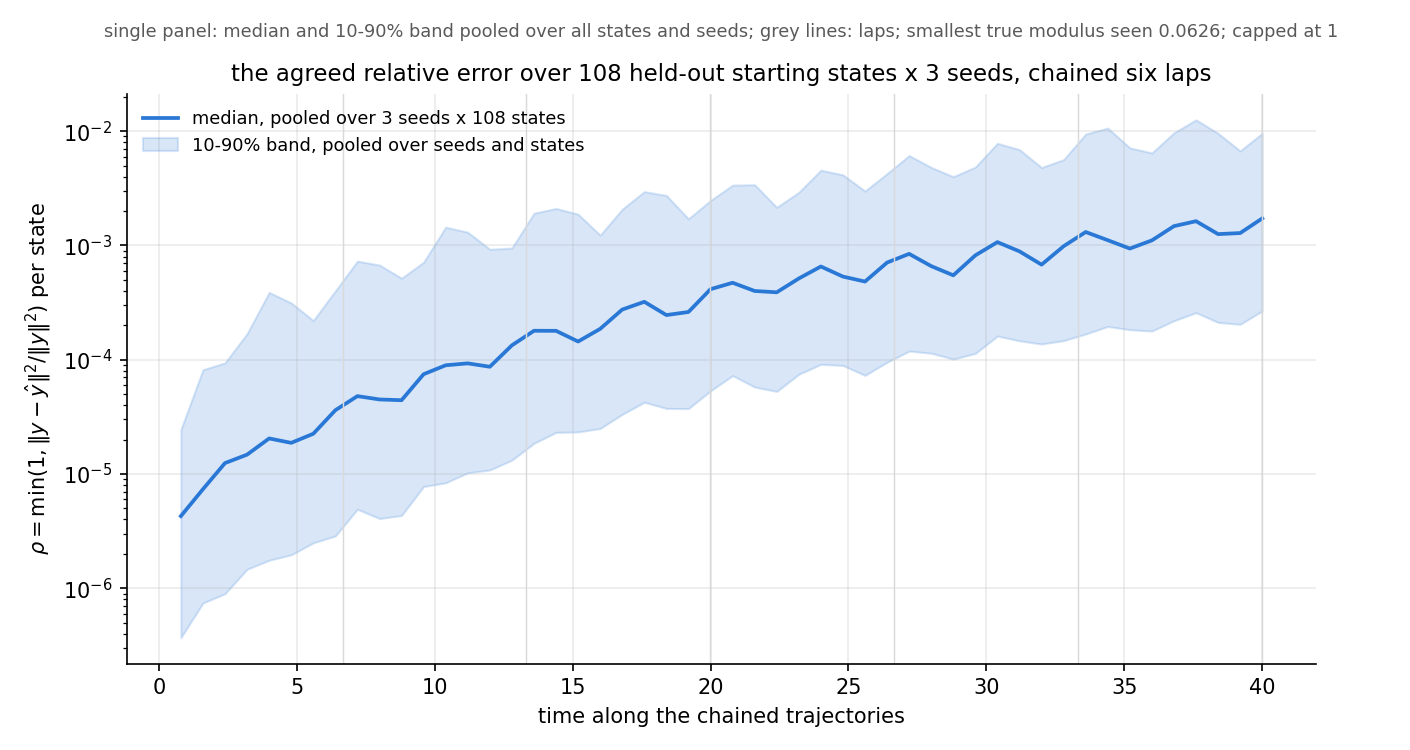
\includegraphics[width=\linewidth]{vdp_test_set.png}
      \srcnote{The error as a distribution: $108$ held-out starts chained six
        periods, median and 10 to 90\% band per seed. Growth lap on lap is the
        behaviour of these three unselected seeds, not a ceiling of the method.}
    \end{column}
    \begin{column}{0.33\textwidth}
      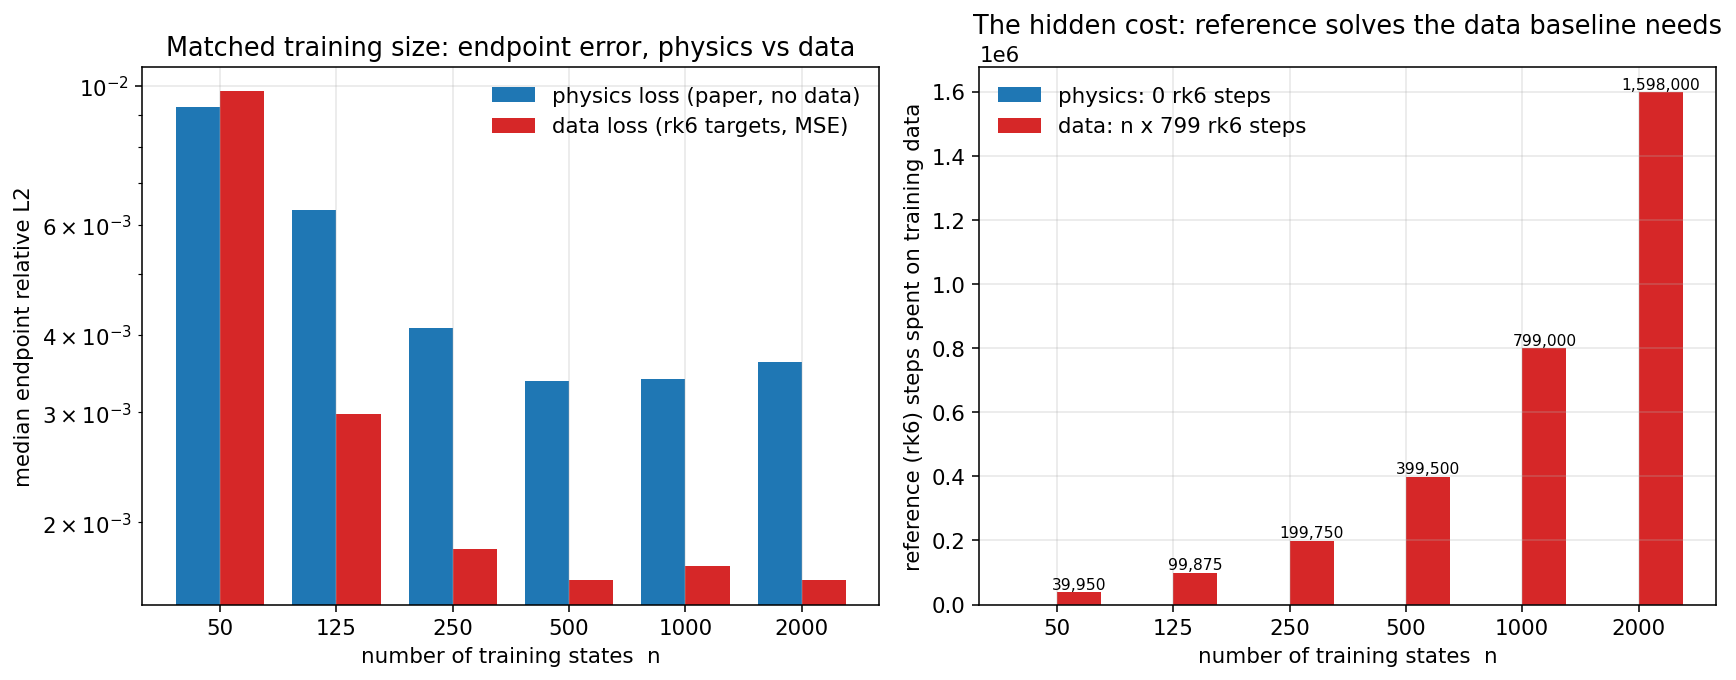
\includegraphics[width=\linewidth]{vdp_data_baseline.png}
      \srcnote{Physics against perfect labels at matched everything else, and
        the reference-integrator work behind the labels: $799$ steps per state.
        The physics variant's bill is zero at every $n$.}
    \end{column}
  \end{columns}
\end{frame}

% ---- 38c: step 0 and 1 on LHCb (added 2026-09-06) ------------------------
\begin{frame}[shrink=25]{Steps 0 and 1 on LHCb: the field along real legs, and the exact scheme's ceiling before any network}
  \vspace{1mm}
  \begin{columns}[T]
    \begin{column}{0.5\textwidth}
      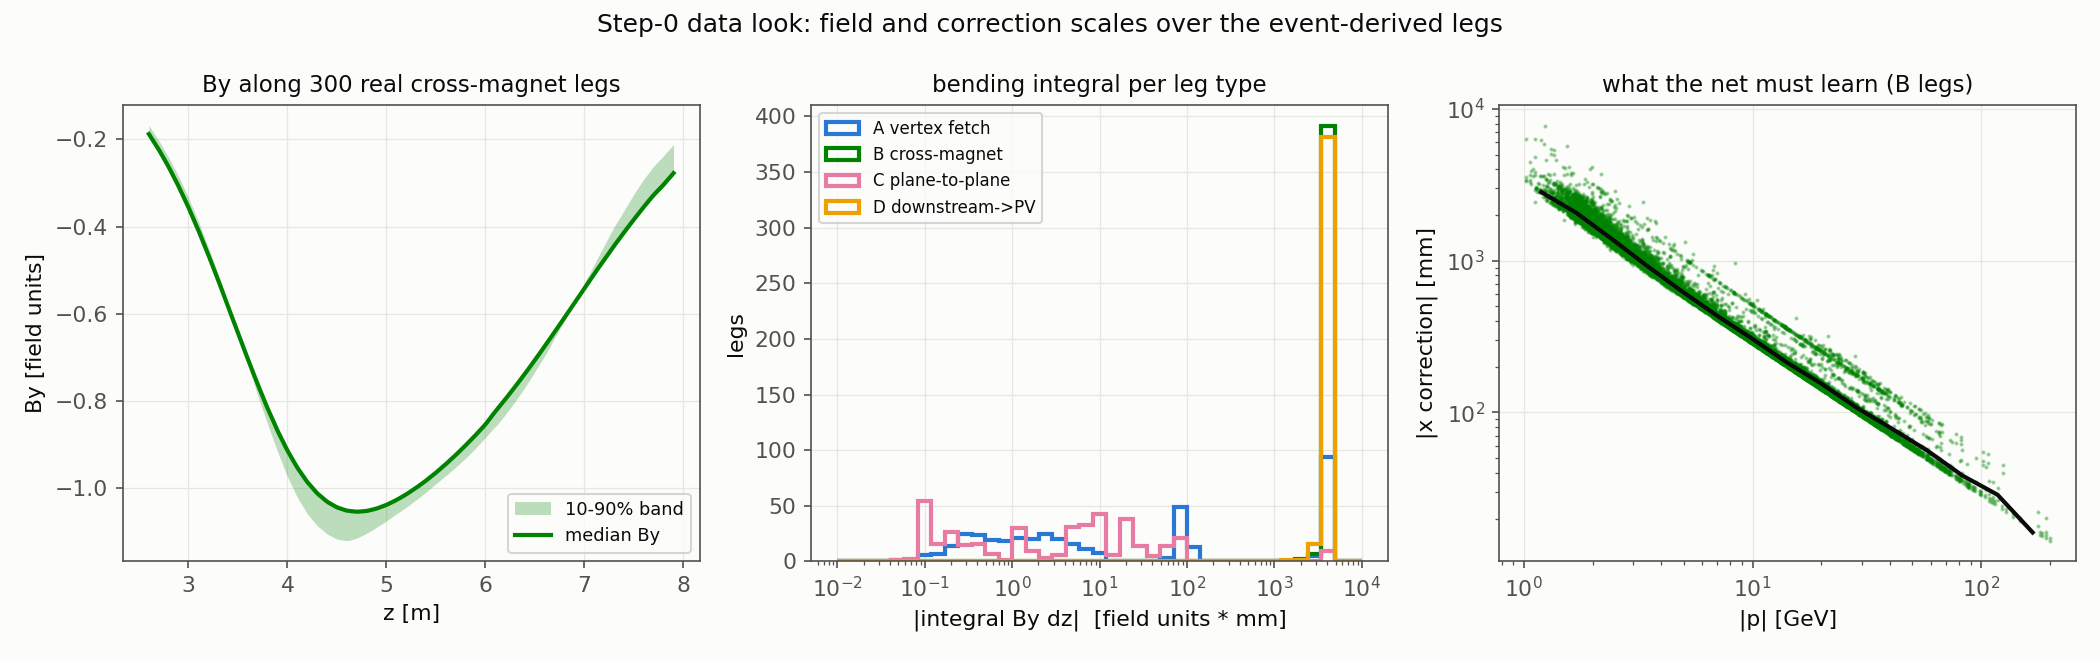
\includegraphics[width=\linewidth]{lhcb_field_along_legs.png}
      \srcnote{The dipole along real leg paths: $|B_y|$ peaks near $1.05$ T at
        $z \approx 4.7$ m and is remarkably uniform across paths. Bending
        integrals separate the leg types by three orders of magnitude, and the
        cross-magnet $x$ correction over the straight line falls as $1/p$, from
        metres at $1$ GeV to about $30\mm$ at $200$ GeV: the function the
        technique must learn.}
    \end{column}
    \begin{column}{0.48\textwidth}
      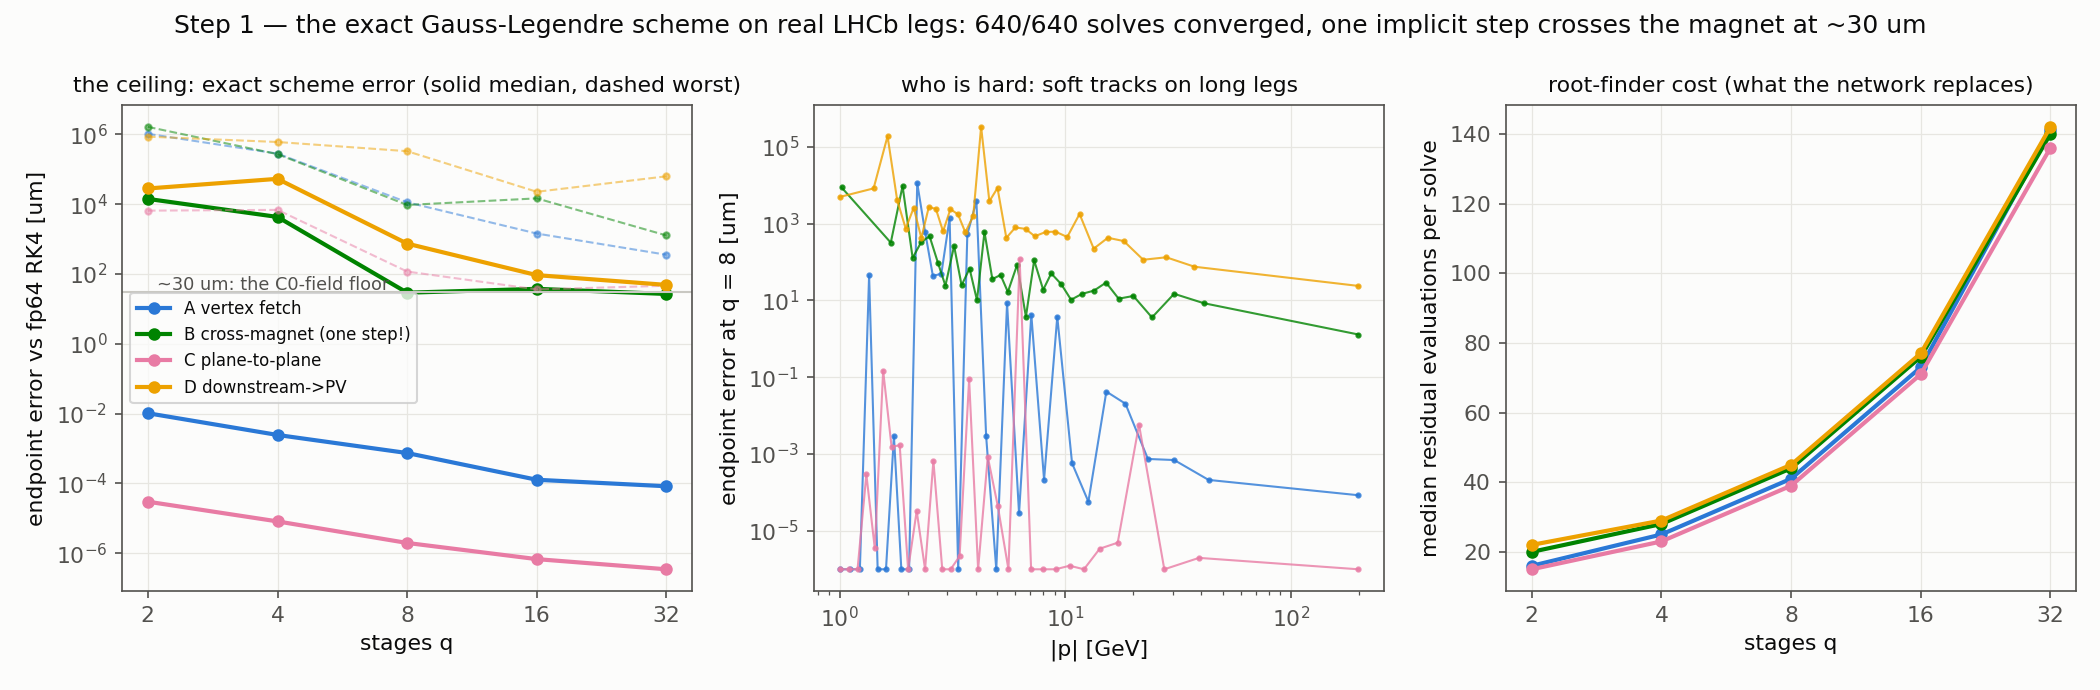
\includegraphics[width=\linewidth]{lhcb_scheme_ceiling.png}
      \srcnote{The Gauss--Legendre scheme solved directly by a root-finder on
        the LHCb equation of motion over real legs, stratified in momentum, no
        network: endpoint error against the fp64 reference per stage count and
        leg type.}
      \begin{itemize}\small
        \item Feasibility: \hl{640 of 640} implicit solves converged on the
              trilinear field, including one giant step across the whole
              magnet.
        \item Ceiling: on the frozen crossing the scheme floors at about
              $23\um$ from $q = 8$ ($29\um$ on the stratified sample). The
              floor is the field map's interpolation, not the scheme.
        \item Everything a network trained on these equations achieves is
              measured against this curve, on the same states.
      \end{itemize}
    \end{column}
  \end{columns}
\end{frame}

% ---- 37 ------------------------------------------------------------------
\begin{frame}[shrink=25]{The July baseline: one frozen magnet crossing, and the two losses indistinguishable}
  \vspace{1mm}
  \begin{columns}[T]
    \begin{column}{0.46\textwidth}
      \centering\small
      \begin{tabular}{@{}lr@{}}
        \toprule
        \multicolumn{2}{@{}l}{frozen leg, $\Delta z = 5177.8\mm$, $q = 8$, $4 \times 50$}\\
        \midrule
        exact scheme (the ceiling) & $23\um$ \\
        network, label-free physics loss & \hl{$183$} \ [$177$, $183$, $235$] \\
        network, supervised data twin & $192$ \ [$162$, $192$, $208$] \\
        straight line (ignore the magnet) & $520{,}444$ \\
        \bottomrule
      \end{tabular}
      \smallskip

      {\small Three things fixed by the end of July, unrevisited since:
       \begin{itemize}\small
         \item \textbf{the leg}: the modal plane pair of the $11{,}046$ forward
               cross-magnet legs, $z_0 = 2648.2\mm$ to $z_1 = 7826.0\mm$, the
               last plane of the upstream tracker to the first of the
               scintillating-fibre tracker. The hardest of the routine steps and
               the one where a surrogate is worth most.
         \item \textbf{$q = 8$}, from the exact-scheme measurement.
         \item \textbf{the first converged label-free result}, with the fiducial
               requirement in place and trained to a confirmed stall.
       \end{itemize}}
    \end{column}
    \begin{column}{0.52\textwidth}
      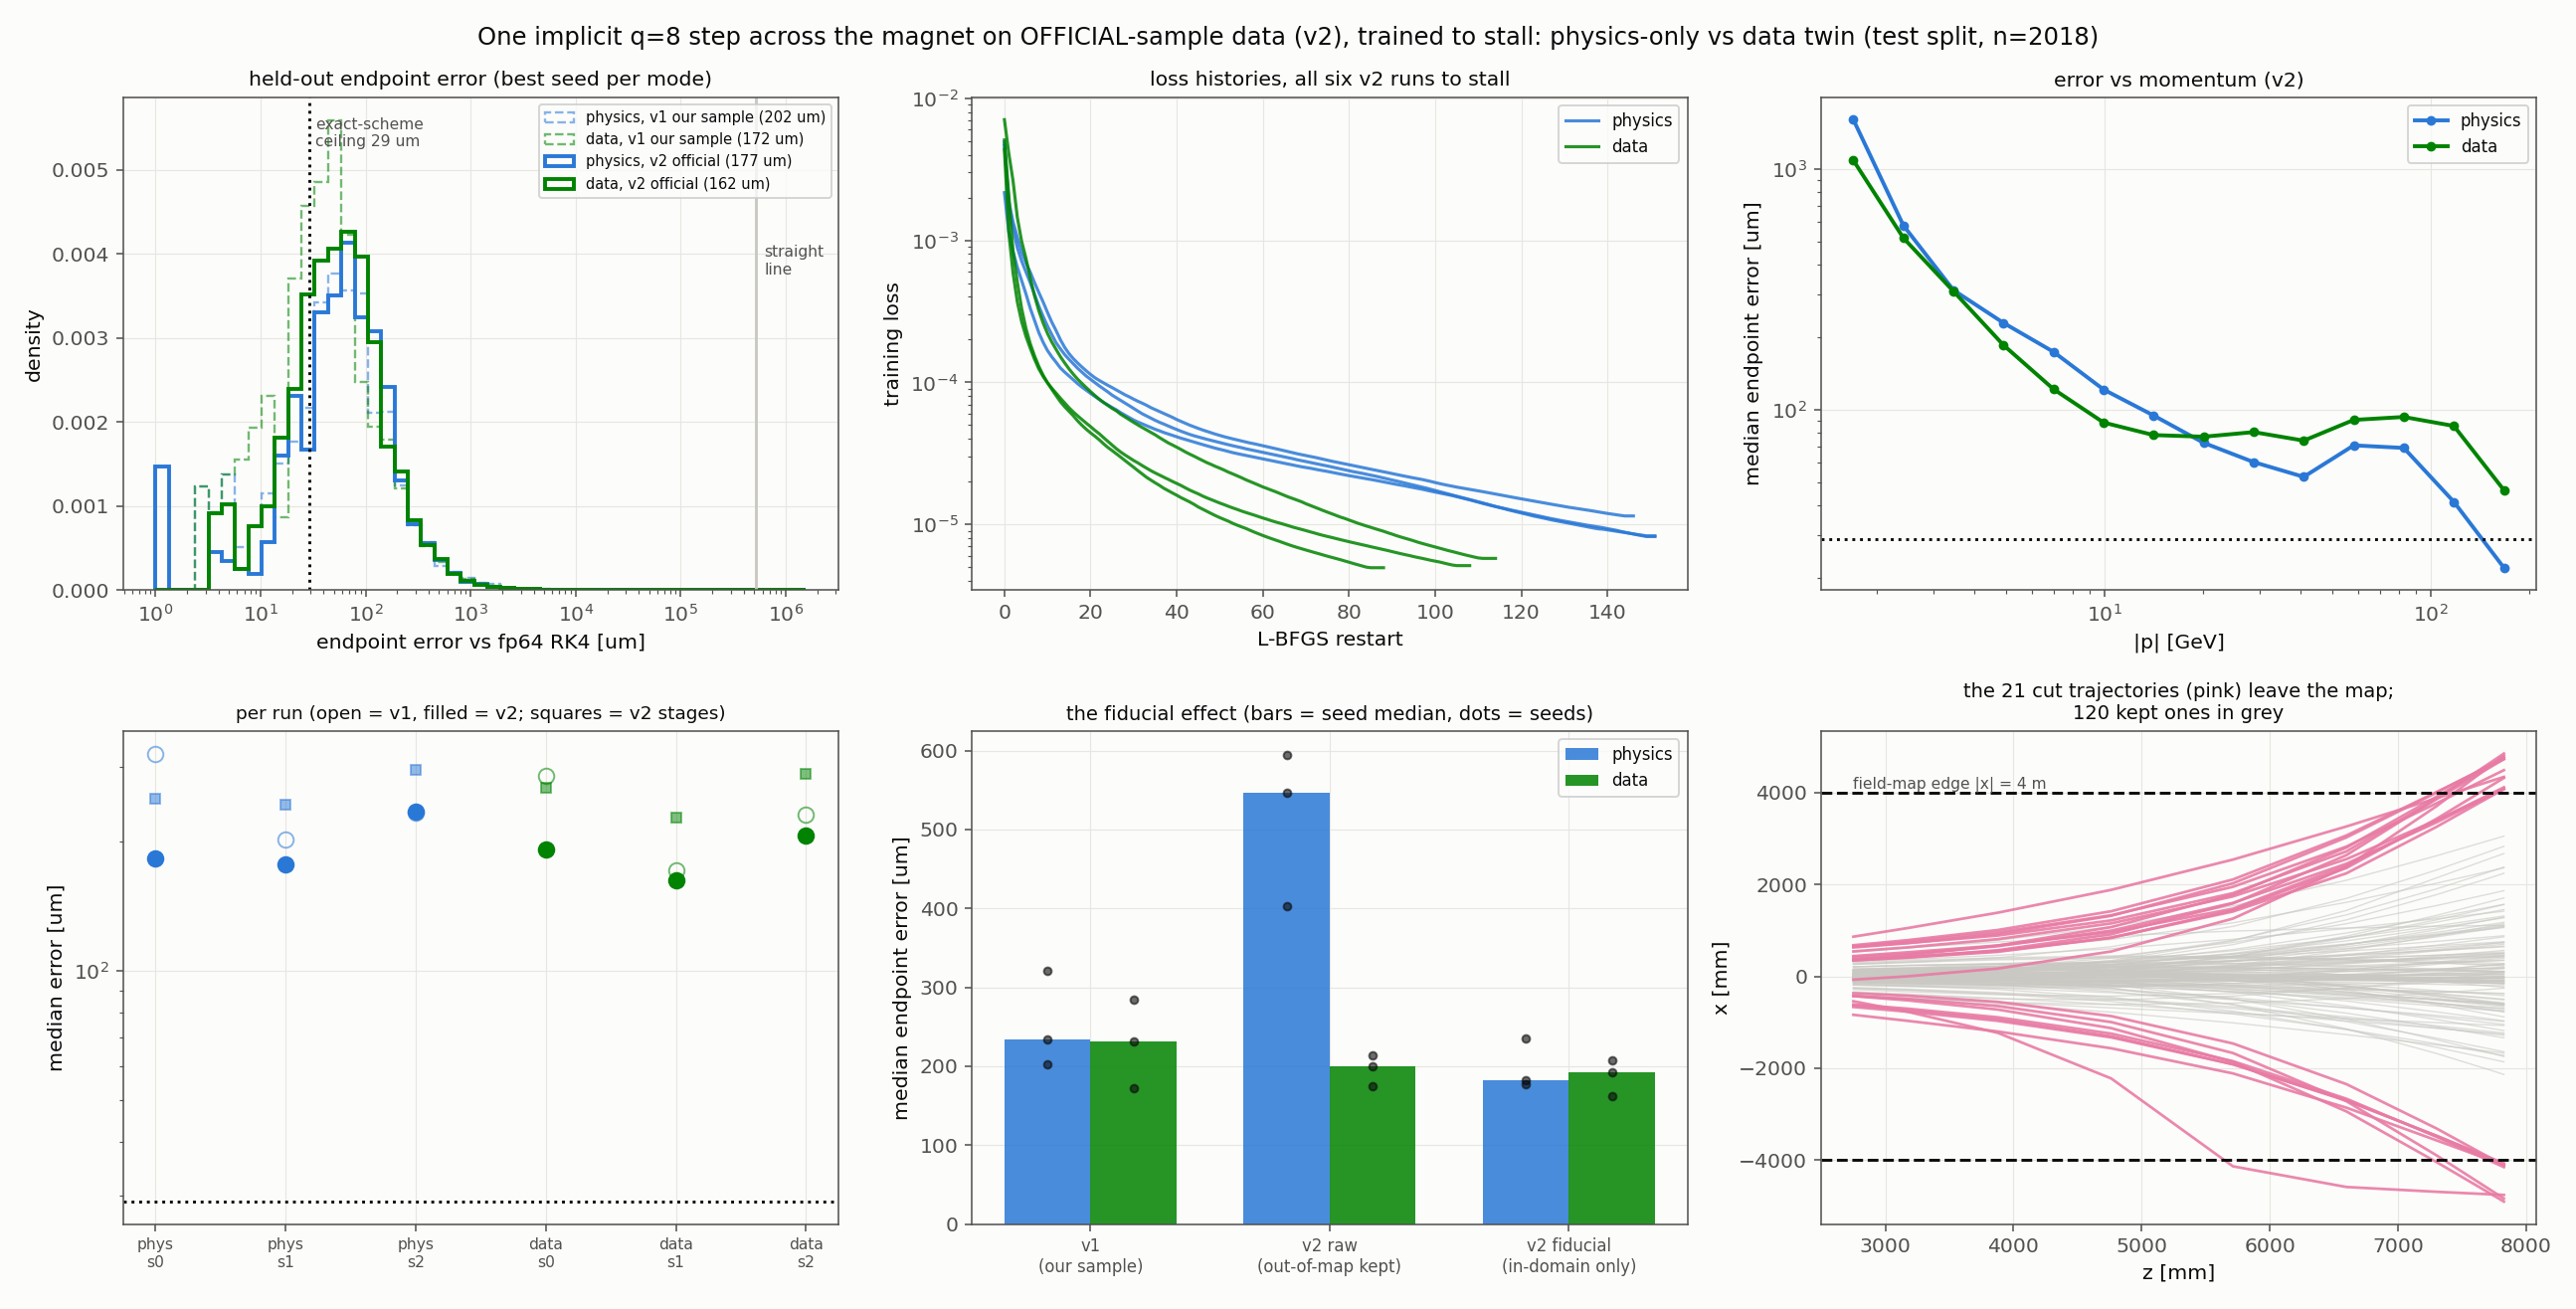
\includegraphics[width=\linewidth]{lhcb_baseline.png}
      \srcnote{Error distributions for the three label-free and three supervised
        seeds; the training histories per optimiser restart with the
        confirmation pass marked; and the comparison against the in-house sample
        the official one replaced.}
      \vspace{-2mm}
      {\small \hl{The point of the figure is the overlap.} With the fiducial
       requirement in place, the label-free loss and the supervised twin are not
       distinguishable at three seeds on this leg. The factor-two gap the July
       experiments chased was a budget artefact.}
    \end{column}
  \end{columns}
\end{frame}

% ---- 38 ------------------------------------------------------------------
\begin{frame}[shrink=25]{Stage-count sweep: at two and four stages the network reproduces the scheme's own error}
  \vspace{2mm}
  \centering\small
  \begin{tabular}{@{}ccccc@{}}
    \toprule
    stages $q$ & physics loss & data twin & exact scheme & exact scheme, 95th pct.\\
    \midrule
    $2$  & \hl{$5202$} [$5199$--$5218$] & $174$ [$168$--$223$] & \hl{$5198$} & $37{,}728$ \\
    $4$  & \hl{$5371$} [$5352$--$5394$] & $181$ [$157$--$181$] & \hl{$5401$} & $54{,}057$ \\
    $8$  & $181$ [$165$--$240$]         & $176$ [$162$--$204$] & $23$   & $1610$ \\
    $16$ & $187$ [$186$--$280$]         & $170$ [$147$--$176$] & $20$   & $325$ \\
    \bottomrule
  \end{tabular}
  \vspace{1mm}

  {\scriptsize Frozen cross-magnet leg, $4\times50$, three seeds each, $24$ runs,
   all converged. Test-split median endpoint error in $\mu$m, median over seeds
   with the seed range in brackets. The ceiling is the same $q$-stage scheme
   solved by root-finder on the very same $2018$ test states. Straight line:
   $520{,}444\um$ at every $q$.}
  \vspace{3mm}

  \begin{columns}[T]
    \begin{column}{0.48\textwidth}
      {\small
      \begin{itemize}\small
        \item At $q = 2$: $5202$ against $5198$, \hl{within $0.1$ percent}. At
              $q = 4$: $5371$ against $5401$, \hl{within $0.6$ percent}.
        \item The network is not failing. It is solving the equations it was
              given, and those equations are $5\mm$ wrong on this leg. This is
              the cleanest available demonstration that the physics loss drives
              the network onto the solution of the discrete scheme, whatever
              that solution happens to be.
        \item The twin at the same $q$ sits at $174$ and $181\um$, thirty times
              better, because its labels are the true trajectory and it never
              sees the scheme at all.
      \end{itemize}}
    \end{column}
    \begin{column}{0.48\textwidth}
      {\small
      \begin{itemize}\small
        \item Between $q = 4$ and $q = 8$ the ceiling crosses \emph{below} the
              network's own floor. From there the network and the optimiser
              limit, and $q = 16$ agrees with $q = 8$ within the seed spread
              while costing $68$ outputs per sample instead of $36$. That fixes
              $q = 8$.
        \item \hl{Two surprises.} $q = 4$ is no better than $q = 2$ and slightly
              worse at the ceiling: formal order $2q$ is asymptotic in small
              steps, and one $5178\mm$ step through a magnet is nowhere near
              that regime. And $q = 16$ is not the hard case to train, $113$ to
              $115$ restarts against $154$; the hardest optimisation in the grid
              is $q = 4$.
        \item The root-finder converged below $10^{-8}$ on $99.9$ percent of
              legs at every $q$, so these are genuine solutions of the discrete
              equations.
      \end{itemize}}
    \end{column}
  \end{columns}
\end{frame}

% ---- 39 ------------------------------------------------------------------
\begin{frame}[shrink=25]{The same sweep as a picture, and why a ceiling must be quoted on the population being scored}
  \vspace{1mm}
  \begin{columns}[T]
    \begin{column}{0.56\textwidth}
      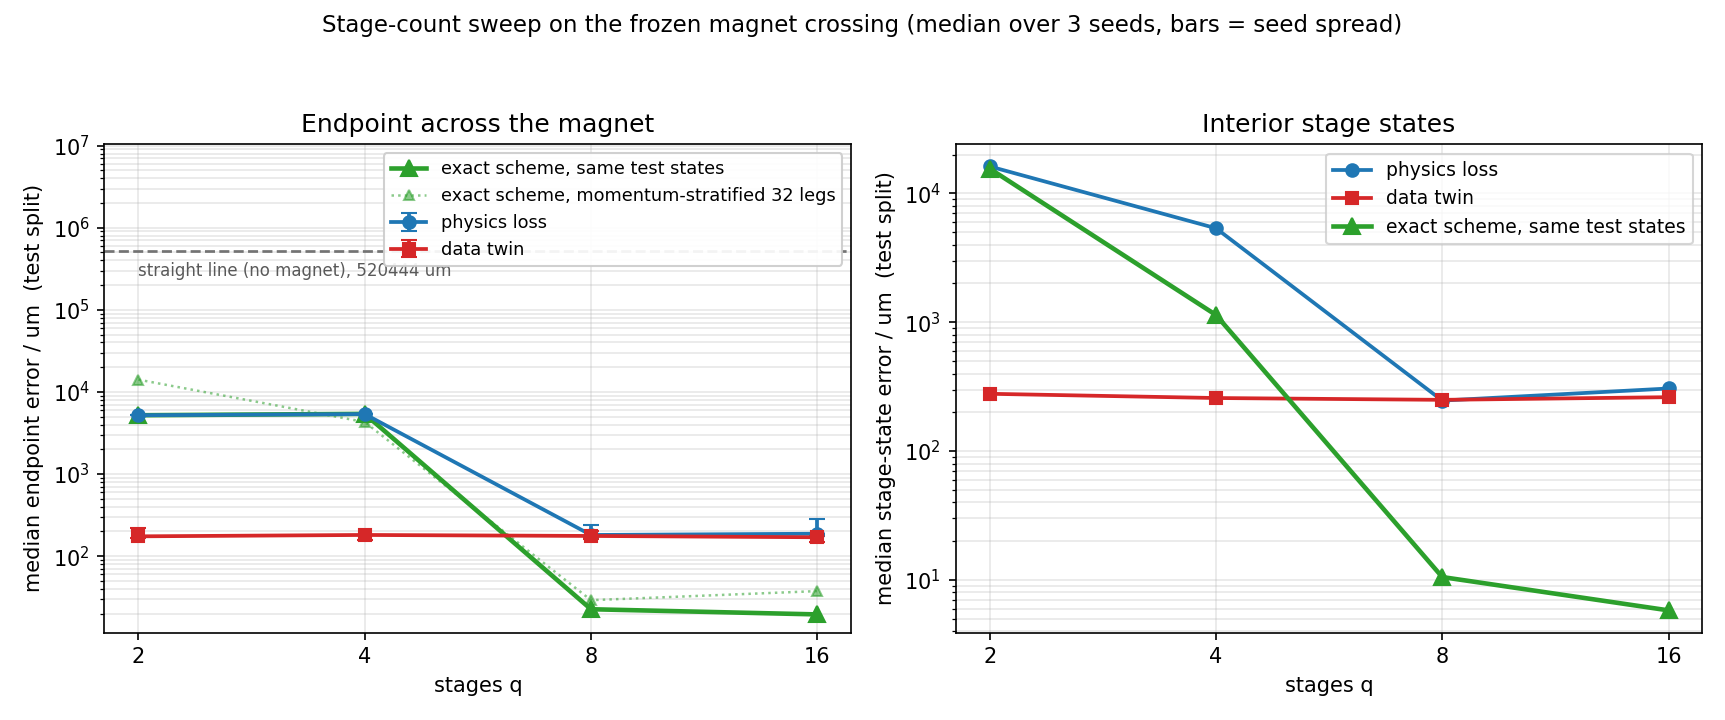
\includegraphics[width=\linewidth]{lhcb_stages.png}
      \srcnote{Left: endpoint error against $q$. Right: the same measure over
        the eight interior stage states. Blue is the label-free loss, red the
        twin, solid green the exact scheme on the very same test states, dotted
        green the same scheme on the momentum-stratified sample of $32$ legs.
        Bars span three seeds; the dashed horizontal line is the straight-line
        baseline.}
    \end{column}
    \begin{column}{0.42\textwidth}
      {\small Blue and green lie on top of one another at $q = 2$ and $q = 4$,
       which is the physics loss reproducing the scheme's own error, and they
       separate at $q = 8$ where the scheme's error drops below the network's
       floor. The red curve is flat at about $175\um$ at every $q$, because the
       twin never sees the scheme.}
      \medskip

      \fbox{\parbox{0.93\textwidth}{\small
        \bad{The $29\um$ correction.} An earlier measurement of the exact
        scheme, made on $32$ legs drawn stratified in momentum and each on its
        own start plane, gave $29\um$ at $q = 8$, and that number was quoted in
        July. Stratifying in momentum deliberately over-weights the soft,
        hard-bending tracks, so it describes a harder population than any test
        split used here.
        \smallskip

        On the $2018$ frozen-leg test states with their natural momentum mix the
        ceiling is \hl{$23\um$}, and the pre-stated ceilings of about $14\mm$ at
        $q = 2$ and $4.3\mm$ at $q = 4$ become $5198$ and $5401\um$. Both curves
        are carried in the figure so the difference is visible rather than
        argued about. The qualitative claim survives intact.}}
    \end{column}
  \end{columns}
\end{frame}

% ---- 40 ------------------------------------------------------------------
\begin{frame}[shrink=25]{The full architecture grid: twelve architectures, ten seeds, 130 runs}
  \vspace{1mm}
  \centering\footnotesize
  \begin{tabular}{@{}llrcrrrl@{}}
    \toprule
    loss & depth $\times$ width & parameters & converged & median & best seed & worst seed & median final loss \\
    \midrule
    physics & $2 \times 32$  & $2{,}436$   & $5/10$  & $1059$ & $853$ & $1600$ & $1.83\times10^{-4}$ \\
    physics & $2 \times 50$  & $4{,}686$   & $9/10$  & $470$  & $340$ & $593$  & $4.54\times10^{-5}$ \\
    physics & $4 \times 32$  & $4{,}548$   & $3/10$  & $411$  & $387$ & $450$  & $5.37\times10^{-5}$ \\
    physics & $6 \times 32$  & $6{,}660$   & $4/10$  & $427$  & $391$ & $2725$ & $6.51\times10^{-5}$ \\
    physics & $4 \times 50$  & $9{,}786$   & $10/10$ & $222$  & $165$ & $244$  & $1.06\times10^{-5}$ \\
    physics & $2 \times 100$ & $14{,}336$  & $10/10$ & $223$  & $201$ & $299$  & $1.08\times10^{-5}$ \\
    physics & $6 \times 50$  & $14{,}886$  & $6/10$  & $326$  & $248$ & $525$  & $2.74\times10^{-5}$ \\
    physics & $4 \times 100$ & $34{,}536$  & $10/10$ & $133$  & $128$ & $156$  & $3.04\times10^{-6}$ \\
    physics & $2 \times 200$ & $48{,}636$  & $10/10$ & $153$  & $128$ & $241$  & $4.19\times10^{-6}$ \\
    physics & $6 \times 100$ & $54{,}736$  & $10/10$ & $191$  & $152$ & $242$  & $9.33\times10^{-6}$ \\
    \hl{physics} & \hl{$4 \times 200$} & $129{,}036$ & $10/10$ & \hl{$115$}  & $100$ & $134$  & $2.06\times10^{-6}$ \\
    physics & $6 \times 200$ & $209{,}436$ & $9/10$  & $159$  & $150$ & $208$  & $6.05\times10^{-6}$ \\
    \midrule
    data twin & $4 \times 200$ & $129{,}036$ & $10/10$ & $128$ & $105$ & $159$ & $1.34\times10^{-6}$ \\
    \bottomrule
  \end{tabular}
  \vspace{2mm}

  {\small Frozen cross-magnet leg at $q = 8$, ordered by parameter count.
   Test-split median endpoint error in $\mu$m over the converged seeds.
   \hl{Unconverged runs are never pooled.} The $24$ label-free runs that did not
   confirm are all at width $32$ or depth $6$, and none of them diverged: they
   failed the confirmation pass, in which a fresh optimiser moves a small or
   deep network again rather than re-stalling.
   \smallskip

   \textbf{Depth 4 is the optimum and it is interior.} Depth $6$ is never better
   and is $39$ to $47$ percent worse at widths $50$, $100$ and $200$; it is also
   much harder to train, $4$, $6$, $10$, $9$ seeds converging against $3$, $10$,
   $10$, $10$ at depth $4$. Depth $2$ is worse at every width, by $33$ percent at
   width $200$ rising to $158$ percent at width $32$.}
\end{frame}

% ---- 41 ------------------------------------------------------------------
\begin{frame}[shrink=25]{The floor is set by the optimiser and not by capacity, and the evidence is one band}
  \vspace{1mm}
  \begin{columns}[T]
    \begin{column}{0.5\textwidth}
      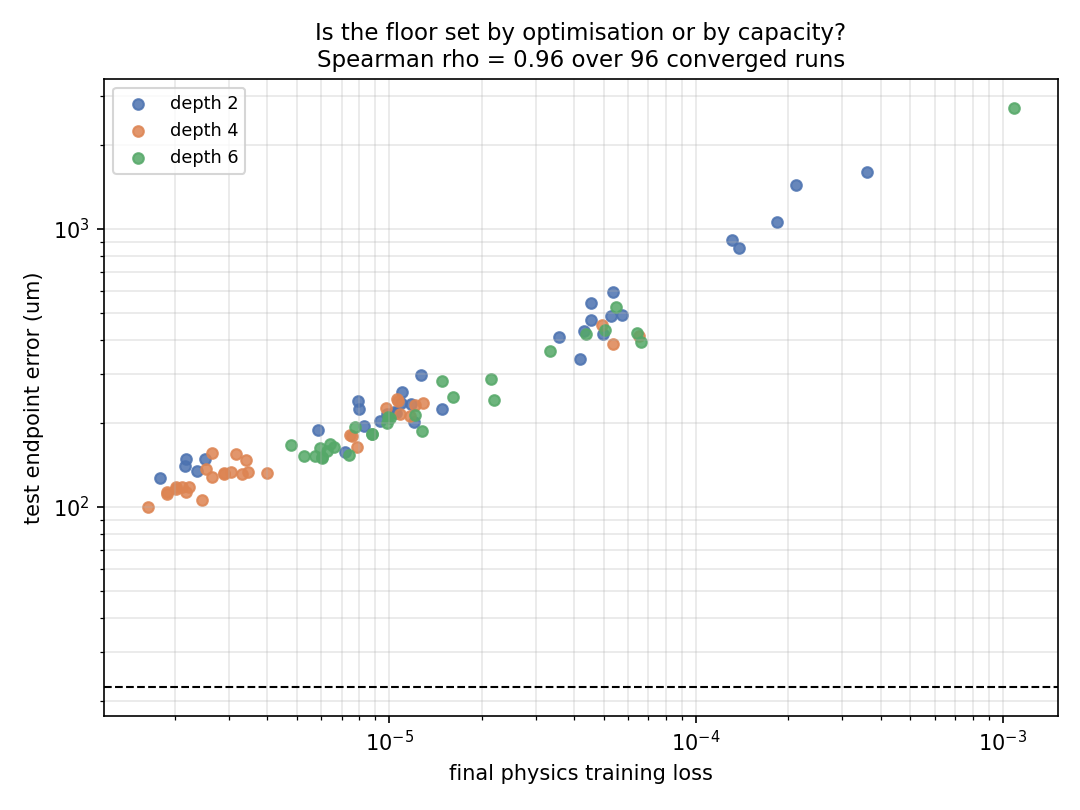
\includegraphics[width=\linewidth]{lhcb_loss_vs_error.png}
      \srcnote{Final training loss against test-split endpoint error, both axes
        logarithmic, one point per converged label-free run, coloured by
        architecture.}
    \end{column}
    \begin{column}{0.48\textwidth}
      \begin{itemize}\small
        \item Over all \hl{$96$ converged label-free runs} the Spearman rank
              correlation between final training loss and test endpoint error is
              \hl{$+0.965$}. Three decades of loss map monotonically onto one
              and a half decades of error.
        \item \hl{If the floor were a capacity limit}, the small architectures
              would sit above the band at their own loss values, forming
              separate branches. They do not. The endpoint error is a readout of
              how far the optimiser got, not of what the network could
              represent.
        \item A wider network helps only because L-BFGS gets further down on it:
              the $4\times50$ networks stall at a median final loss of
              $1.06\times10^{-5}$, the $4\times200$ networks at
              $2.06\times10^{-6}$.
        \item \hl{The prediction that follows}, and which the residual redesign
              then tested: anything improving the \emph{conditioning} of the
              optimisation problem should pay more than more parameters do.
      \end{itemize}
      \smallskip
      {\footnotesize This is the same number, to the second decimal place, that
       the van der Pol study measured on a two-dimensional autonomous oscillator
       with an analytic right-hand side. I did not expect two systems with that
       little in common to agree that closely, and I have no explanation for it
       beyond the shared optimiser.}
    \end{column}
  \end{columns}
\end{frame}

% ---- 41b -----------------------------------------------------------------
\begin{frame}[shrink=25]{Returns collapse with size, and at the largest size the label-free loss overtakes its twin}
  \vspace{1mm}
  \begin{columns}[T]
    \begin{column}{0.46\textwidth}
      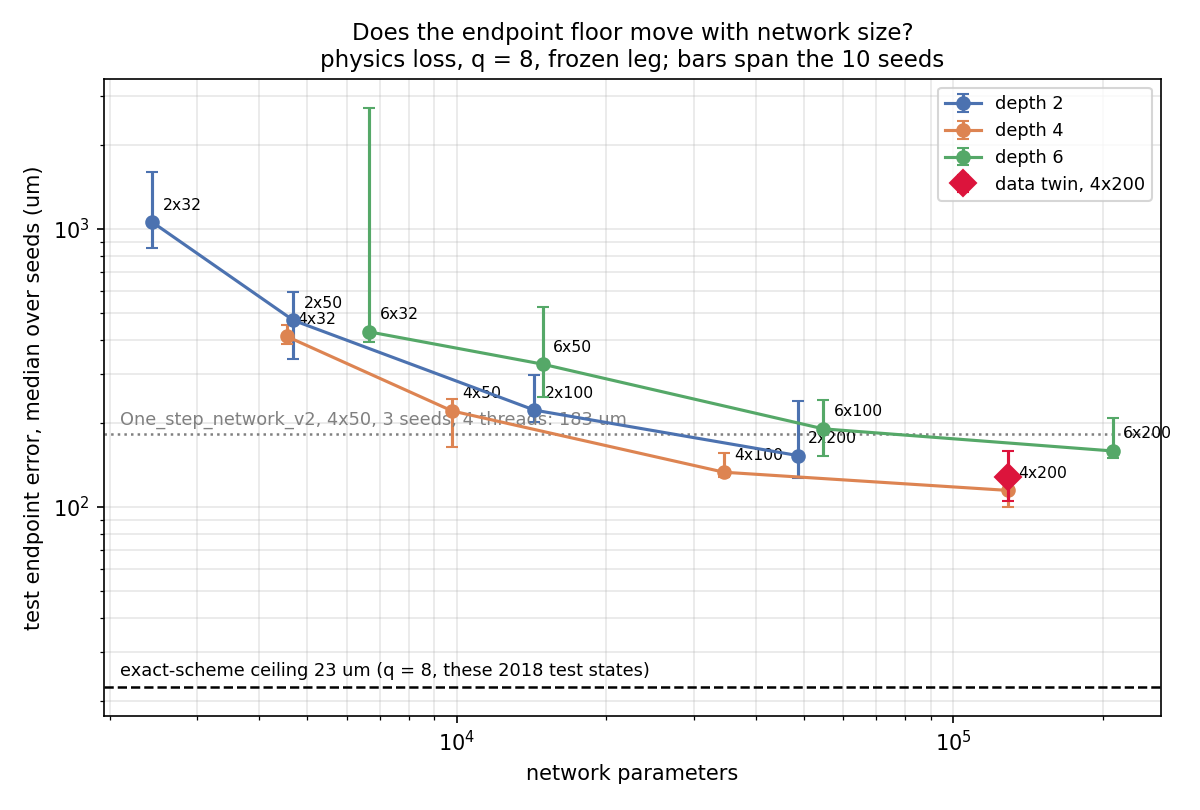
\includegraphics[width=\linewidth]{lhcb_architecture.png}
      \srcnote{Median test endpoint error against parameter count, both axes
        logarithmic. Each point is one architecture; the three curves are depths
        $2$, $4$ and $6$; bars span ten seeds. The red diamond is the supervised
        twin at $4\times200$. The dotted line is the July three-seed baseline at
        $183\um$; the dashed line at the bottom is the exact-scheme ceiling at
        $23\um$ on the same $2018$ test states.}
    \end{column}
    \begin{column}{0.52\textwidth}
      \begin{itemize}\small
        \item Growing from $2436$ to $129{,}036$ parameters, a factor $53$,
              moves the median from $1059$ to $115\um$, a factor $9.2$. The last
              width doubling buys \hl{$14$ percent for $3.7$ times the
              parameters} and $1.8$ times the wall time.
        \item The depth-$4$ curve flattens above about thirty thousand
              parameters, and \hl{the gap between the flattening curve and the
              ceiling is the factor $5$} this study attributes to the optimiser.
        \item \hl{At $4\times200$ the label-free loss beats its own supervised
              twin}: $115\um$ [$100$--$134$] against $128\um$ [$105$--$159$], so
              the twin's median is $12$ percent higher. The twin also has the
              wider seed spread, a factor $1.51$ between best and worst against
              $1.33$, while reaching its stall in about half the restarts. The
              factor-two gap the July experiments chased is gone.
        \item \hl{Seeds must be pooled.} Over architectures with at least three
              converged seeds the median luckiest-to-unluckiest ratio is $1.54$,
              shrinking with size to $1.22$ at $4\times100$.
        \item \hl{Validation selection is safe for the one-step task}: rank
              correlation between validation and test endpoint error is
              $+0.995$ over the $96$ runs, the validation-best seed is also the
              test-best in $9$ of $12$ architectures, and where it is not the
              penalty is at most $2.3$ percent. \bad{That stops being true the
              moment the network is chained.}
      \end{itemize}
      \smallskip
      {\footnotesize The recommendation this produced: $4\times100$ as the
       smallest adequate network, with $4\times200$ as the check that a result
       is not size-limited. $4\times50$ sits on the steep part of the curve,
       where a result reports the network size as much as the physics.}
    \end{column}
  \end{columns}
\end{frame}

% ---- 42 ------------------------------------------------------------------
\begin{frame}[shrink=25]{Training where no labels exist: the magnet-up polarity, the sample's own, reaches the same floor}
  \vspace{2mm}
  \centering\small
  \begin{tabular}{@{}lrr@{}}
    \toprule
    quantity & magnet up (the sample's own) & magnet down (as labelled) \\
    \midrule
    network, label-free physics loss & \hl{$229$} [$171$--$296$], 10 seeds & \hl{$222$} [$165$--$244$], 10 seeds \\
    network, supervised data twin    & $204$ [$187$--$230$], 3 seeds  & $192$ [$162$--$208$], 3 seeds \\
    exact-scheme ceiling on the test states & $22.1$ & $22.5$ \\
    straight line & $525{,}184$ & $520{,}444$ \\
    network divided by its own ceiling & $10.4\times$ [$7.7$--$13.4$] & $9.8\times$ [$7.2$--$10.8$] \\
    fiducial removals, train / validation / test & \bad{$0$ / $0$ / $0$} & $21$ / $20$ / $15$ \\
    exact scheme, worst case & $38\mm$ & $258\mm$ \\
    \bottomrule
  \end{tabular}
  \vspace{2mm}

  \begin{columns}[T]
    \begin{column}{0.48\textwidth}
      {\footnotesize \textbf{Design.} Identical $4\times50$ network, identical
       protocol, identical training population; the single change is that the
       loss is built on the reversed map. Ten label-free seeds plus three
       supervised controls, $13$ runs, all converged. The reversed-polarity
       references exist only to score; the label-free runs never see them.
       \smallskip

       \textbf{Three checks before submitting.} The two maps are exactly one
       another's negative: on $200{,}000$ random in-map points the maximum of
       $|\mathbf{B}_{\mathrm{up}} + \mathbf{B}_{\mathrm{down}}|$ is $0.0$ in all
       three components. Both polarities are built from the same event rows,
       since the selection uses no field. And a probe run established that the
       polarity flag really reaches the loss: one restart from the same seed
       gives $2.62\times10^{-3}$ reversed against $8.03\times10^{-3}$ original.}
    \end{column}
    \begin{column}{0.48\textwidth}
      {\footnotesize The two ten-seed ranges overlap almost completely, and the
       four percent difference in medians is far inside a seed spread that is
       itself a factor $1.7$ wide reversed and $1.5$ original. Both are three
       orders of magnitude below the straight line, so \hl{the network learned
       the bending and not merely the geometry, and it learned it with the
       correct sign.}
       \smallskip

       \bad{One genuine asymmetry, and it is in the tracks rather than the map.}
       The fiducial requirement removes $21$, $20$ and $15$ states on the
       original polarity and none on the reversed one: the sample's charge and
       angular distribution is not symmetric in $x$, and the original polarity
       is the one that bends these particular soft tracks out of the map while
       the reversed bends them back in. A control re-scoring the reversed
       networks on only the tracks the original also keeps moves the median from
       $229.4$ to $226.6\um$, about one percent, so medians are unaffected.
       Statements about \emph{tails}, however, must say which polarity.
       \smallskip

       \bad{Correction, 6 September.} Magnet up is the sample's own polarity,
       so this is the only experiment here scored against the physically right
       field. The numbers are unchanged; the framing is.}
    \end{column}
  \end{columns}
\end{frame}

% ---- 43 ------------------------------------------------------------------
\begin{frame}[shrink=25]{The reversed polarity in pictures: same distribution, same momentum curve, opposite bend}
  \vspace{2mm}
  \centering
  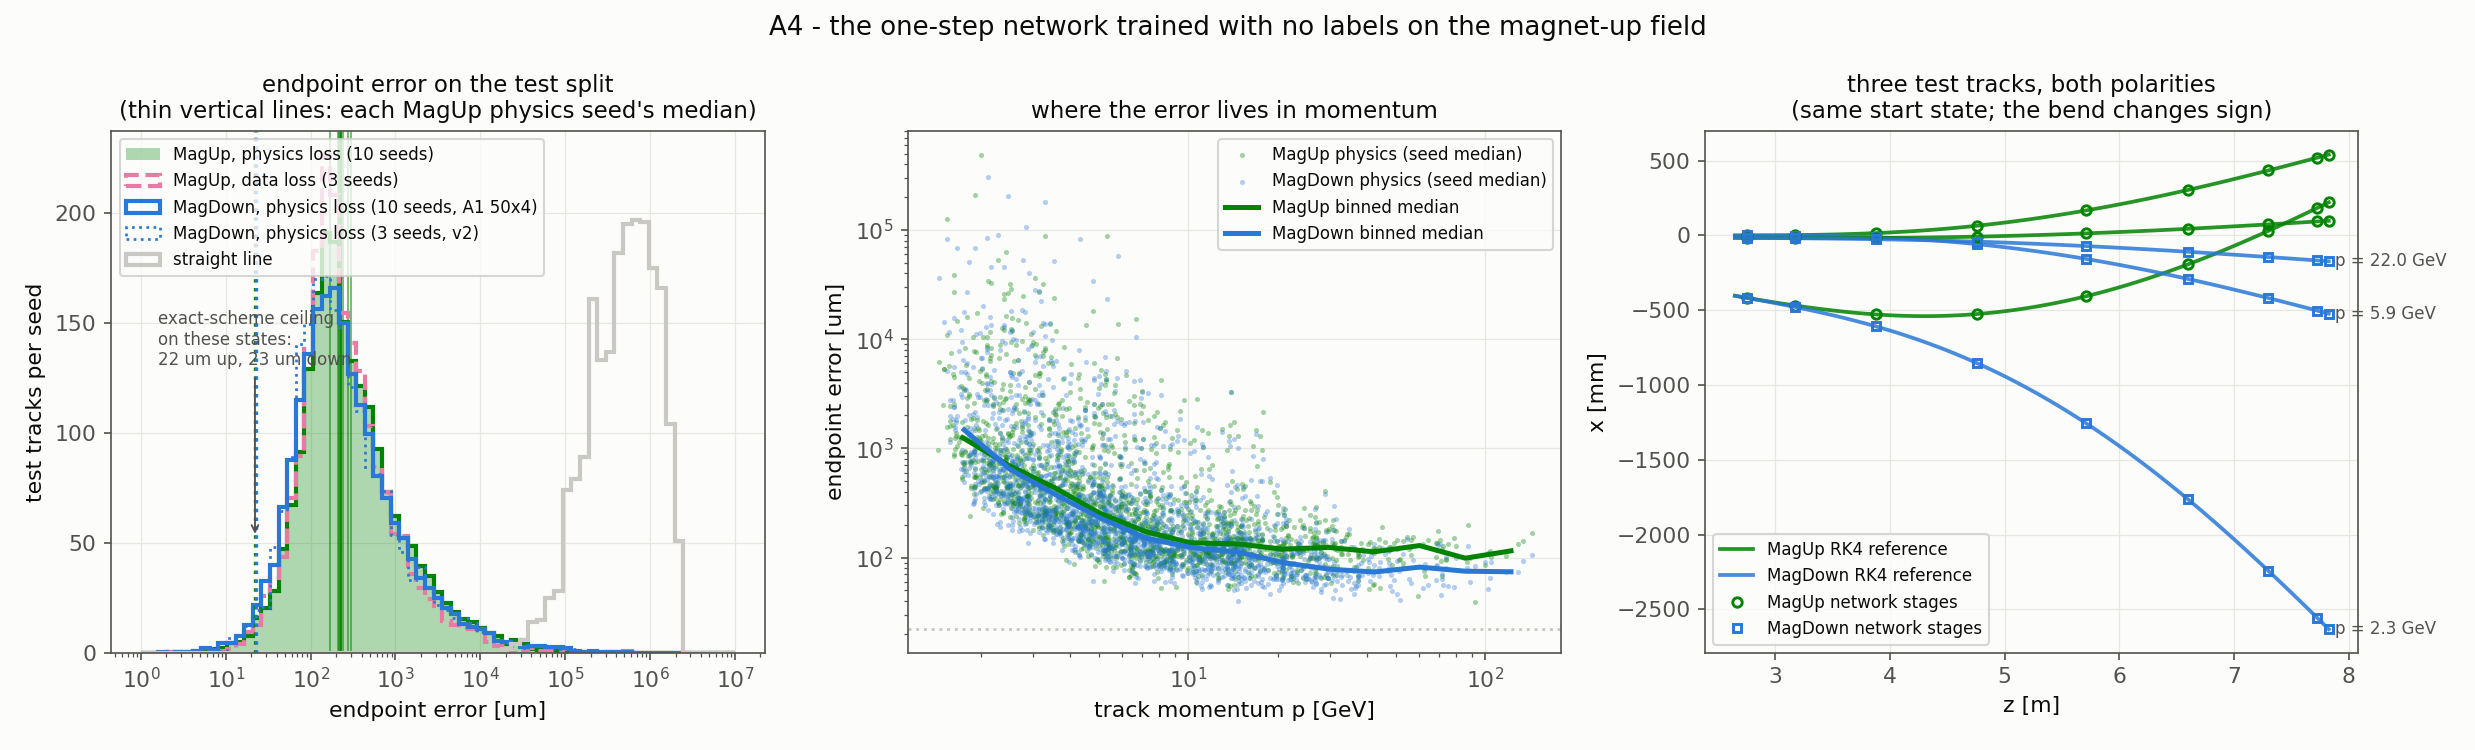
\includegraphics[width=0.95\linewidth]{lhcb_magnet_up.png}
  \srcnote{Left: the distribution of test-split endpoint errors on a logarithmic
    axis, with the ten reversed-polarity label-free seeds in filled green, the
    three reversed supervised seeds dashed, the ten original-polarity label-free
    seeds solid blue, the three July original seeds dotted, and the
    straight-line baseline in grey near one million micrometres. The two
    polarities lie on top of one another and the two ceilings, $22$ and
    $23\um$, are marked at the left. Middle: endpoint error against track
    momentum with binned medians overlaid; the two polarities trace the same
    curve, falling from about one millimetre at $2$ GeV to about $100\um$ above
    $20$ GeV. Right: three test tracks propagated from the same start states
    under both polarities, with the network's eight stage states as markers on
    the reference curves. The trajectories curve in opposite directions, which
    is the check that the network learned the sign of the bending.}
\end{frame}

% ---- 44 ------------------------------------------------------------------
\begin{frame}[shrink=25]{One network for every kind of step, absolute outputs: worse than a straight line on short steps}
  \vspace{2mm}
  \centering\small
  \begin{tabular}{@{}lrrrrrrrr@{}}
    \toprule
    & \multicolumn{3}{c}{physics loss} & \multicolumn{3}{c}{data twin} & & \\
    \cmidrule(lr){2-4}\cmidrule(lr){5-7}
    leg & $4\times50$ & $4\times100$ & $4\times200$ & $4\times50$ & $4\times100$ & $4\times200$ & straight & ceiling \\
    \midrule
    A vertex fetch, $341\mm$   & $849$  & $404$  & $229$  & $653$  & $385$ & $227$ & \hl{$10.9$}  & $0.0013$ \\
    B cross-magnet, $5175\mm$  & $6742$ & $2600$ & $1740$ & $2395$ & $933$ & $777$ & $444{,}075$ & $46$ \\
    C plane-to-plane, $70\mm$  & $535$  & $300$  & $213$  & $486$  & $235$ & $182$ & \hl{$6.6$}   & $6\times10^{-7}$ \\
    \bottomrule
  \end{tabular}
  \vspace{1mm}

  {\scriptsize Median $\mu$m over converged seeds. The leg becomes an input:
   each sample carries its own $z_0$ and $\Delta z$, normalised, and the stage
   planes become per-sample quantities $z_0 + c_j \Delta z$. Training size fixed
   by a rule stated before any result was seen: the largest of $2000$, $4000$,
   $8000$, $16000$ for which one restart runs under $90$ seconds, giving
   $N = 8000$, or $7935 / 3969 / 3961$ states after the fiducial cut. Leg mix is
   the training set's own and is not stratified: $1317$ A, $1060$ B, $5558$ C.
   Ten label-free seeds and three supervised at $4\times50$ and $4\times100$
   ($26$ runs, all converged); a second wave at $4\times200$ ($13$ runs, $12$
   converged).}
  \vspace{2mm}

  \begin{columns}[T]
    \begin{column}{0.48\textwidth}
      {\small
      \begin{itemize}\small
        \item One label-free network does serve all three leg types, and nowhere
              near any of their ceilings. Against the frozen-leg network on the
              same kind of leg, making the leg an input \hl{costs a factor
              $14$}, and a factor $11.7$ against the ten-seed frozen figure of
              $222\um$ even though this network is twice as wide.
        \item On the two short types \bad{the network is worse than doing
              nothing}, and the widest is still $32$ times (C) and $21$ times
              (A) worse than ignoring the magnet.
      \end{itemize}}
    \end{column}
    \begin{column}{0.48\textwidth}
      {\small
      \begin{itemize}\small
        \item Width keeps paying with clear diminishing returns: leg B goes
              $6742 \to 2600 \to 1740$, factors $2.6$ then $1.5$, still $38$
              times above its $46\um$ ceiling.
        \item \hl{The twin is uniformly ahead here}, by a factor $2.8$ on leg B
              at $4\times100$, where on the frozen leg the two were
              indistinguishable. The gap opens exactly where the leg geometry
              varies.
      \end{itemize}}
    \end{column}
  \end{columns}
\end{frame}

% ---- 45 ------------------------------------------------------------------
\begin{frame}[shrink=25]{The hypothesis that experiment produced: it is the output parameterisation, not the capacity}
  \vspace{1mm}
  \begin{columns}[T]
    \begin{column}{0.53\textwidth}
      \textbf{Stated before testing.} The general-leg network is limited by
      predicting the \emph{absolute} state at each stage, scaled by a single
      population-wide constant per component. Four pieces of evidence:
      \begin{enumerate}\small
        \item The output scale on the general dataset is $602\mm$ in $x$ and
              $341\mm$ in $y$, set by the whole population and dominated by the
              $5$ m crossings. The correction the network must produce on a
              $70\mm$ hop is about $7\um$. \hl{Resolving $7\um$ on an output
              whose scale is $602\mm$ is one part in $10^{8}$.} On the frozen
              dataset the scale is $396\mm$ and the correction $520\mm$: a
              completely different regime.
        \item The error is roughly a fixed fraction of the largest step in
              training, not of each step: $404$, $2600$, $300\um$ on legs whose
              true corrections span five orders of magnitude.
      \end{enumerate}
    \end{column}
    \begin{column}{0.45\textwidth}
      \begin{enumerate}\small
        \setcounter{enumi}{2}
        \item On the short legs the error is \emph{flat} across the eight Gauss
              nodes, the signature of an offset. On the long leg it grows
              monotonically to the endpoint, roughly doubling, which is a bend
              being under-resolved.
        \item The frozen-leg network, same architecture, loss, optimiser and
              data source but one geometry and therefore a matched scale, is a
              factor $14$ better on that geometry.
      \end{enumerate}
      \medskip
      \fbox{\parbox{0.93\textwidth}{\small
        \textbf{The alternative was capacity, and the second wave separated
        them.} The size study predicted width would buy about $14$ percent over
        $4\times100$ on the frozen leg; on the general dataset it bought a
        factor $1.5$ on leg B, \hl{leaving the factor $14$ largely intact and
        the short legs still an order of magnitude worse than a straight line.}
        That is consistent with the parameterisation hypothesis and not with the
        capacity one.}}
    \end{column}
  \end{columns}
\end{frame}

% ---- 46 ------------------------------------------------------------------
\begin{frame}[shrink=25]{Chaining the absolute-output network along real particle paths: the error doubles per leg}
  \vspace{2mm}
  \centering\small
  \begin{tabular}{@{}crrrrrrr@{}}
    \toprule
    & \multicolumn{3}{c}{physics loss} & \multicolumn{3}{c}{data twin} & \\
    \cmidrule(lr){2-4}\cmidrule(lr){5-7}
    legs walked & $4\times50$ & $4\times100$ & $4\times200$ & $4\times50$ & $4\times100$ & $4\times200$ & particles \\
    \midrule
    $1$ & $440$      & $246$      & $174$      & $388$      & $217$   & $165$   & $4563$ \\
    $2$ & $1423$     & $783$      & $540$      & $1275$     & $652$   & $510$   & $4563$ \\
    $3$ & $2562$     & $1443$     & $1029$     & $2225$     & $1051$  & $894$   & $4563$ \\
    $4$ & $3919$     & $2293$     & $1738$     & $3634$     & $1484$  & $1490$  & $4563$ \\
    $5$ & $8163$     & $4831$     & $4133$     & $6991$     & $2869$  & $2972$  & $2914$ \\
    $6$ & $14{,}479$ & $8904$     & $8659$     & $10{,}087$ & $4820$  & $5695$  & $1481$ \\
    $7$ & $15{,}999$ & $10{,}248$ & $10{,}450$ & $10{,}739$ & $5283$  & $6476$  & $853$ \\
    \bottomrule
  \end{tabular}
  \vspace{1mm}

  {\scriptsize Median endpoint error against the reference path, test split, in
   $\mu$m. All $4563$ particles contribute up to leg $4$, so the first four rows
   are the like-for-like comparison. Construction: collect the planes named by
   each test particle's stored forward legs, sort them, call consecutive planes
   a leg. $4563$ particles with four or more legs, $23{,}500$ legs, median leg
   length $70\mm$, 99th percentile $5.2$ m. The obvious rule of butting rows
   together is unusable: only $15$ of $7636$ test particles have four rows that
   butt exactly.}
  \vspace{2mm}

  \begin{columns}[T]
    \begin{column}{0.48\textwidth}
      {\small \hl{Nothing breaks and nothing saturates.} No chain diverges and
       the 95th percentile grows at the same rate as the median. Step-to-step
       growth ratios at $4\times100$ are $3.2$, $1.8$, $1.6$, $2.1$, $1.8$,
       $1.1$, essentially the same at every architecture and both losses.
       \bad{That is not the square-root growth of independent random errors; it
       is systematic}, each leg starting from an already displaced state and
       adding its own bias. Over a full path the network is $5$ to $10\mm$ out,
       and width shifts the curve down without changing its slope.}
    \end{column}
    \begin{column}{0.48\textwidth}
      {\small \hl{Chaining also changes how a seed must be chosen.} The cheap
       one-step validation error, an excellent selector for the one-step task,
       carries \emph{no} information about chained performance: rank correlation
       $0.08$ at $4\times100$, and the best one-step seed is only sixth best
       when chained. The validation \emph{chain} error transfers almost
       perfectly, $0.92$ and $0.95$ at the two architectures and $0.94$ at
       $4\times200$. A seed must be selected on the quantity that will actually
       be used, which is the same lesson the oscillator taught.}
    \end{column}
  \end{columns}
\end{frame}

% ---- 47 ------------------------------------------------------------------
\begin{frame}[shrink=25]{Leg D: replacing a hard step by two easier ones makes it worse, under both designs}
  \vspace{2mm}
  \centering\small
  \begin{tabular}{@{}lrrrrrr@{}}
    \toprule
    & \multicolumn{3}{c}{absolute outputs} & \multicolumn{3}{c}{straight-line residual} \\
    \cmidrule(lr){2-4}\cmidrule(lr){5-7}
    & physics $4{\times}100$ & twin $4{\times}100$ & physics $4{\times}200$
    & physics $4{\times}100$ & twin $4{\times}100$ & physics $4{\times}50$ \\
    \midrule
    two composite steps & $59{,}416$ & $33{,}416$ & $35{,}034$ & \hl{$4252$} & $2374$ & $4768$ \\
    the same leg in one giant step & $8778$ & $3158$ & $4563$ & \hl{$3749$} & $2213$ & $3806$ \\
    \midrule
    \multicolumn{7}{@{}l}{exact $q = 8$ scheme on these legs: $752$; \quad $q = 16$: $216$; \quad straight line: $948{,}000$} \\
    \bottomrule
  \end{tabular}
  \vspace{1mm}

  {\scriptsize Median $\mu$m over $2726$ test particles. Leg D is the single
   backward step from the first post-magnet plane to the collision vertex,
   median length $-8.6$ m. \hl{No leg of this geometry was in any training set},
   so this is an out-of-training test by construction. The stored label agrees
   with a fresh reference pass to $0.045\um$.}
  \vspace{2mm}

  \begin{columns}[T]
    \begin{column}{0.48\textwidth}
      {\small \textbf{Under absolute outputs.} Composite stepping is four to ten
       times \emph{worse} than the single giant step, and both are more than an
       order of magnitude above the ceiling. The reason is visible in the first
       hop, which is longer than any leg in training and is already $1.5$ to
       $10\mm$ out. \hl{This is not a sign problem}: the network has seen
       backward steps, since all $1317$ A legs and $490$ of the $1060$ B legs
       are backward. It is that no leg-D geometry was in training at all. It
       does still beat the straight line by a factor $100$ to $300$.}
    \end{column}
    \begin{column}{0.48\textwidth}
      {\small \textbf{Under the residual design.} The composite improves by a
       factor $14$, from $59.4$ to $4.3\mm$, far more than the single step's
       factor $2.3$: the composite's first hop is a $-6.4$ m backward step,
       longer than any B leg, and it went from $4.1$ to $1.5\mm$, while its
       second hop is vertex-fetch-like, exactly where the residual arm gained a
       factor $92$. \hl{The gap has closed from a factor $6.8$ to $1.13$}, so
       the earlier conclusion that composite stepping actively destroys accuracy
       is now only marginally true. Both remain five times the ceiling, and the
       95th percentile barely moved, $142$ against $149\mm$.}
    \end{column}
  \end{columns}
\end{frame}

% ---- 48b -----------------------------------------------------------------
\begin{frame}[shrink=25]{The absolute-output network in pictures: by leg, chained, and on the giant step}
  \vspace{1mm}
  \begin{columns}[T]
    \begin{column}{0.34\textwidth}
      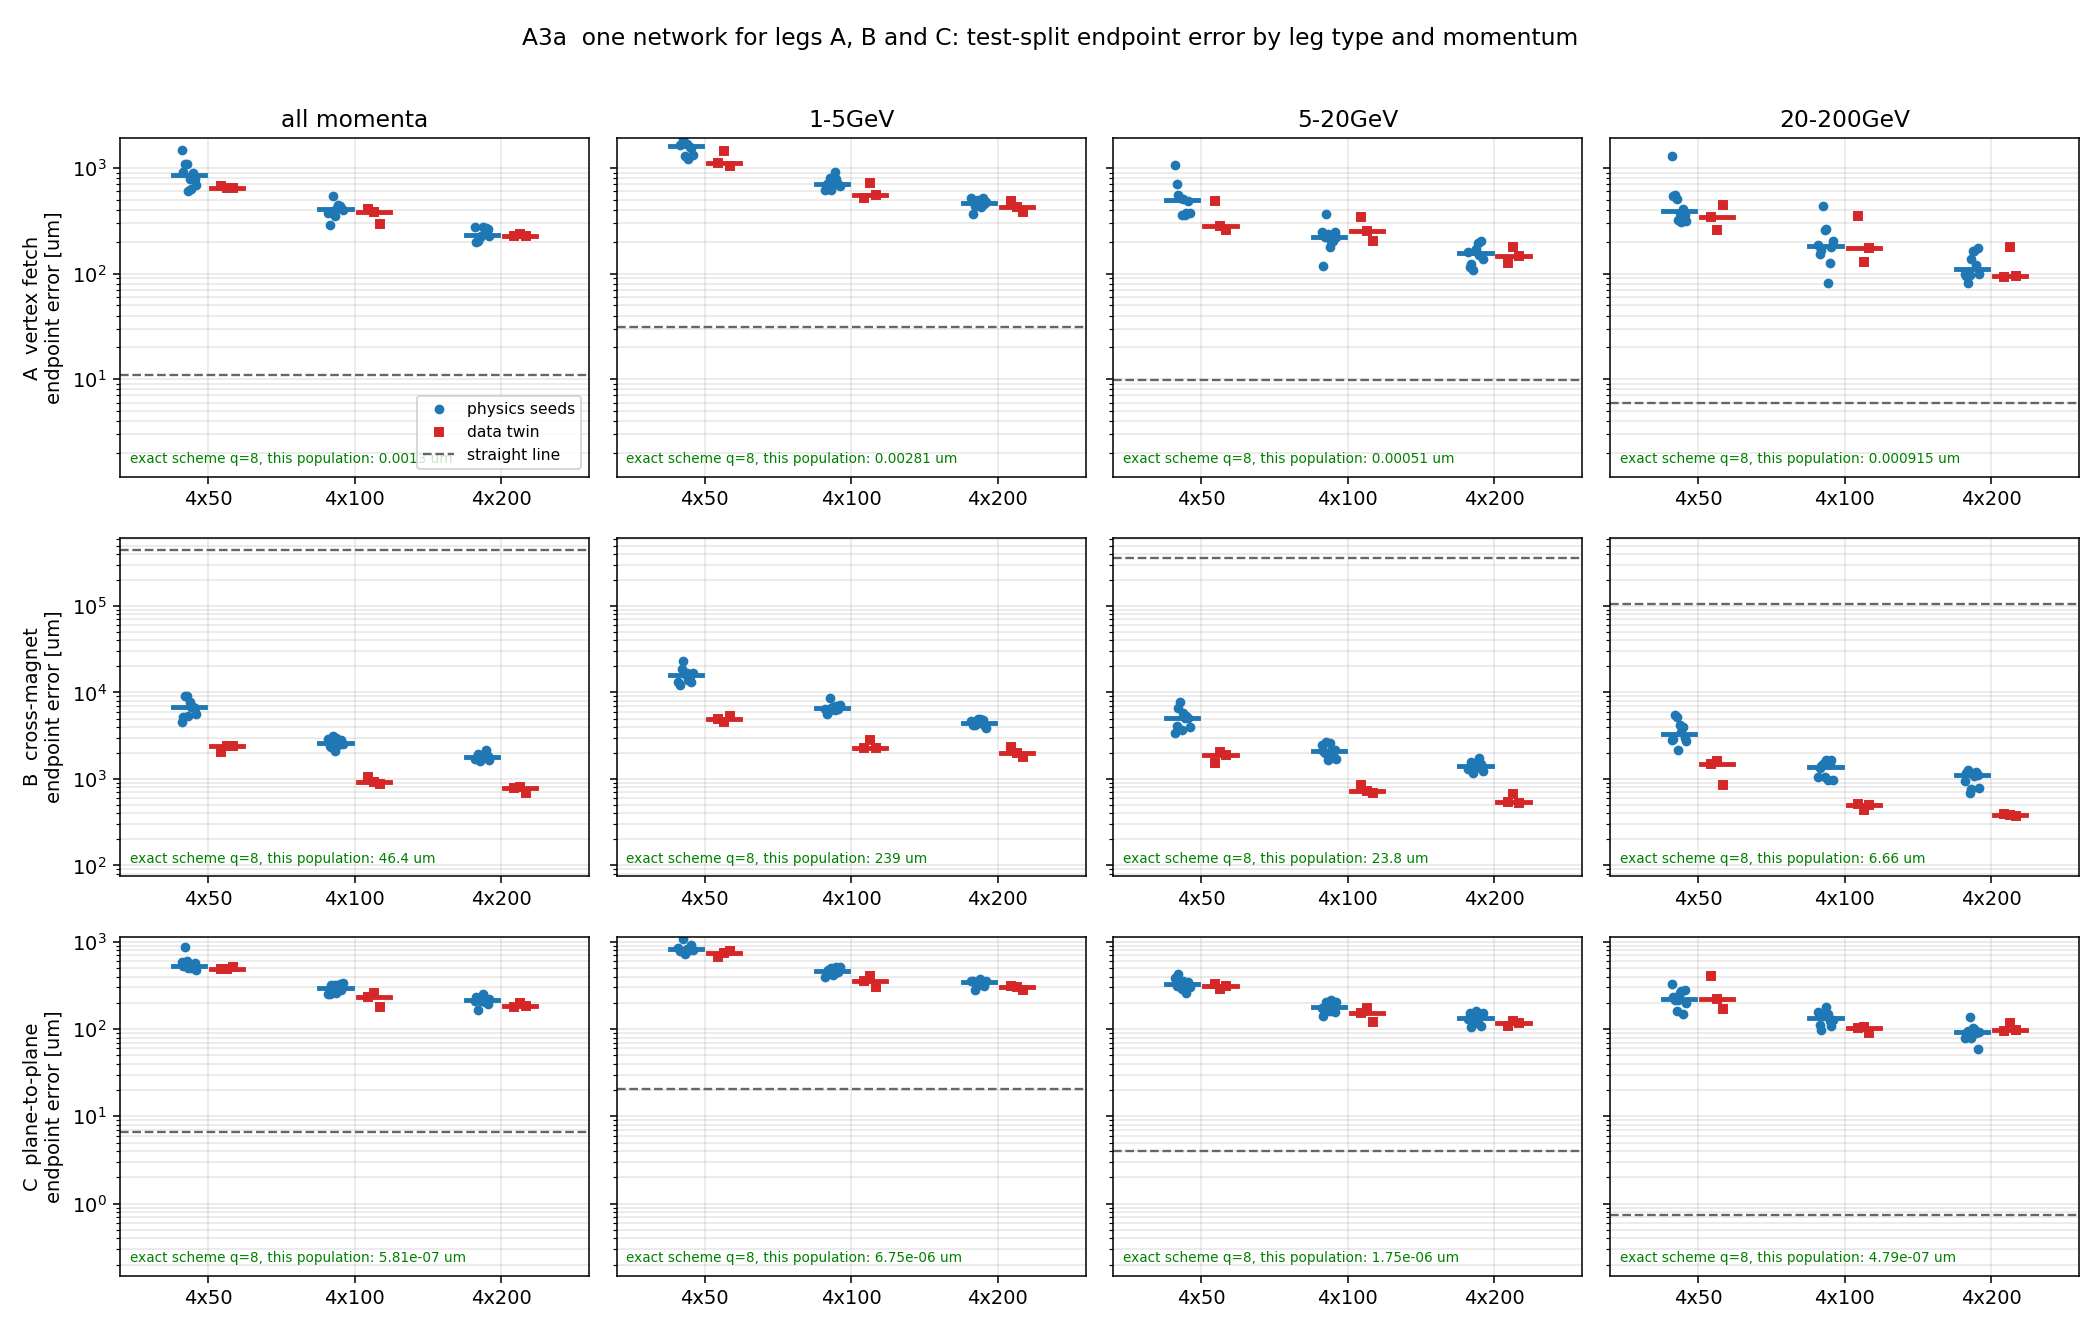
\includegraphics[width=\linewidth]{lhcb_general_legs.png}
      \srcnote{Endpoint error by leg type (rows: A vertex fetch, B cross-magnet,
        C plane-to-plane) and momentum band (columns: all momenta, then $1$--$5$,
        $5$--$20$ and $20$--$200$ GeV). Blue: ten label-free seeds. Red: three
        supervised seeds. Dashed grey: the straight line. Green: the
        exact-scheme ceiling on that same population. \bad{On the top and bottom
        rows the straight line lies below every network point.}}
    \end{column}
    \begin{column}{0.34\textwidth}
      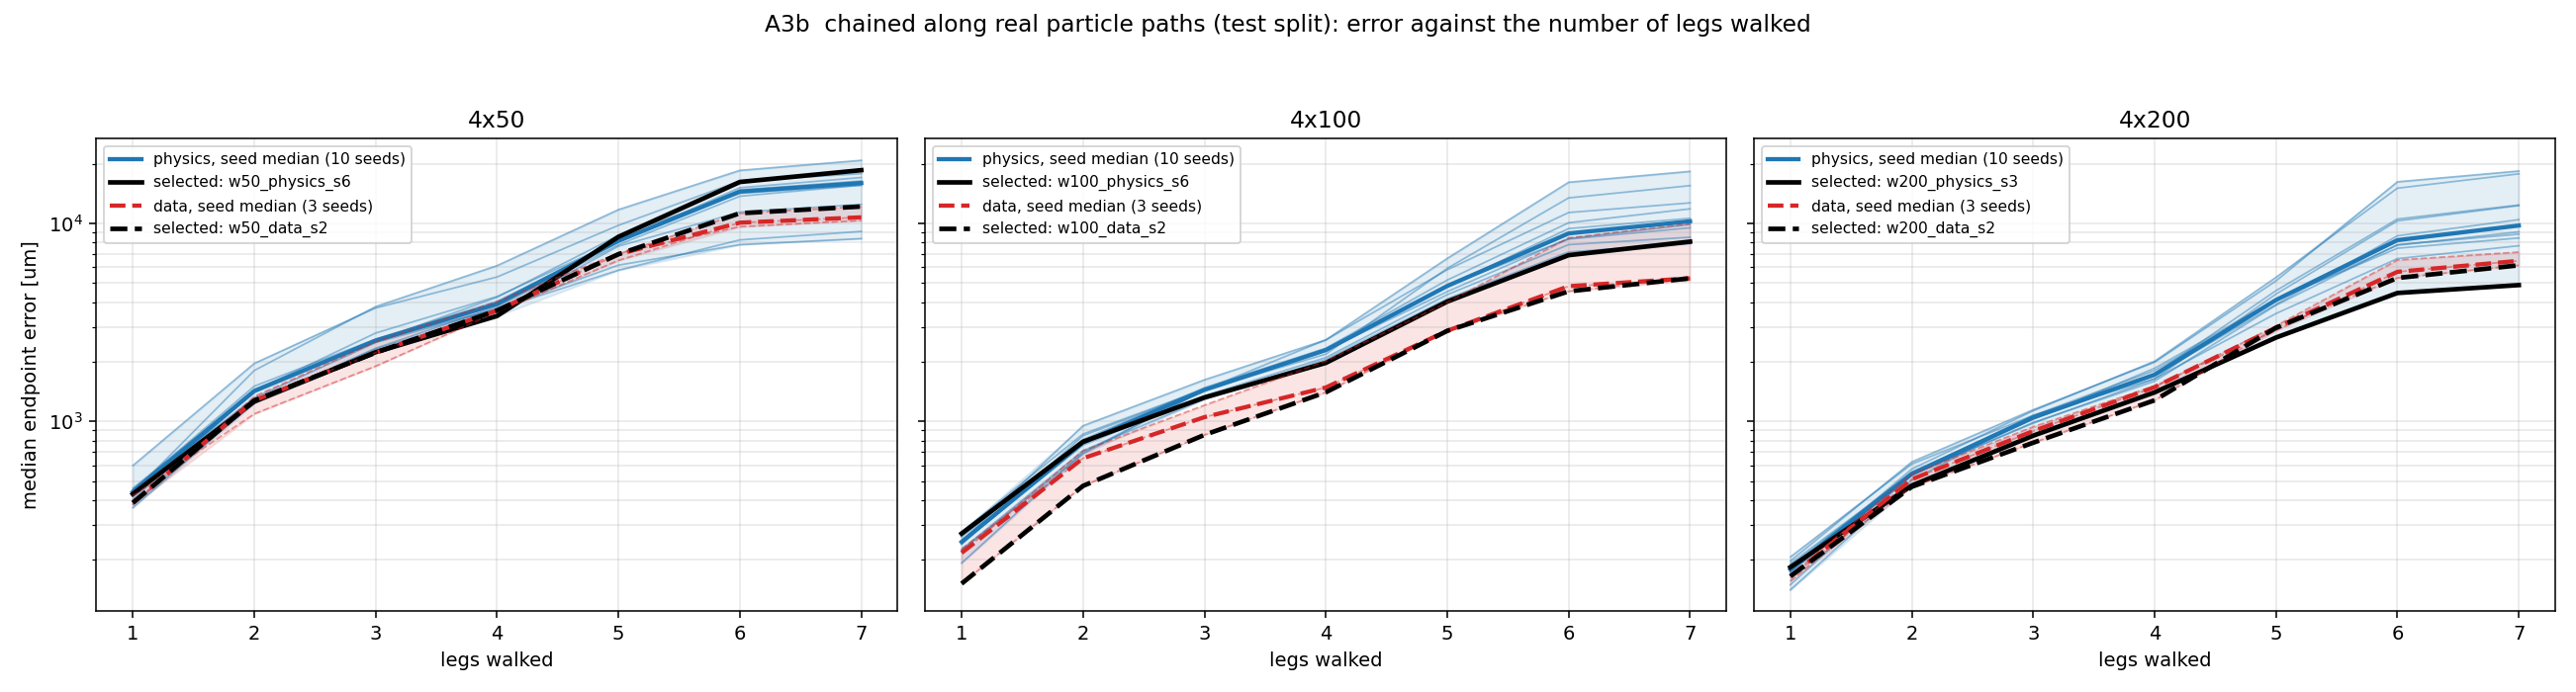
\includegraphics[width=\linewidth]{lhcb_chains.png}
      \srcnote{Median endpoint error against the number of legs walked. Each
        curve is one architecture and loss; bands are the seed spread, dashed
        curves the 95th percentiles. The contributing-particle count falls after
        leg four, marked on the axis. \hl{The curves are straight on this axis
        over the first four legs, which is geometric growth}: the error roughly
        doubles per leg rather than growing like the square root of the number
        of legs.}
    \end{column}
    \begin{column}{0.30\textwidth}
      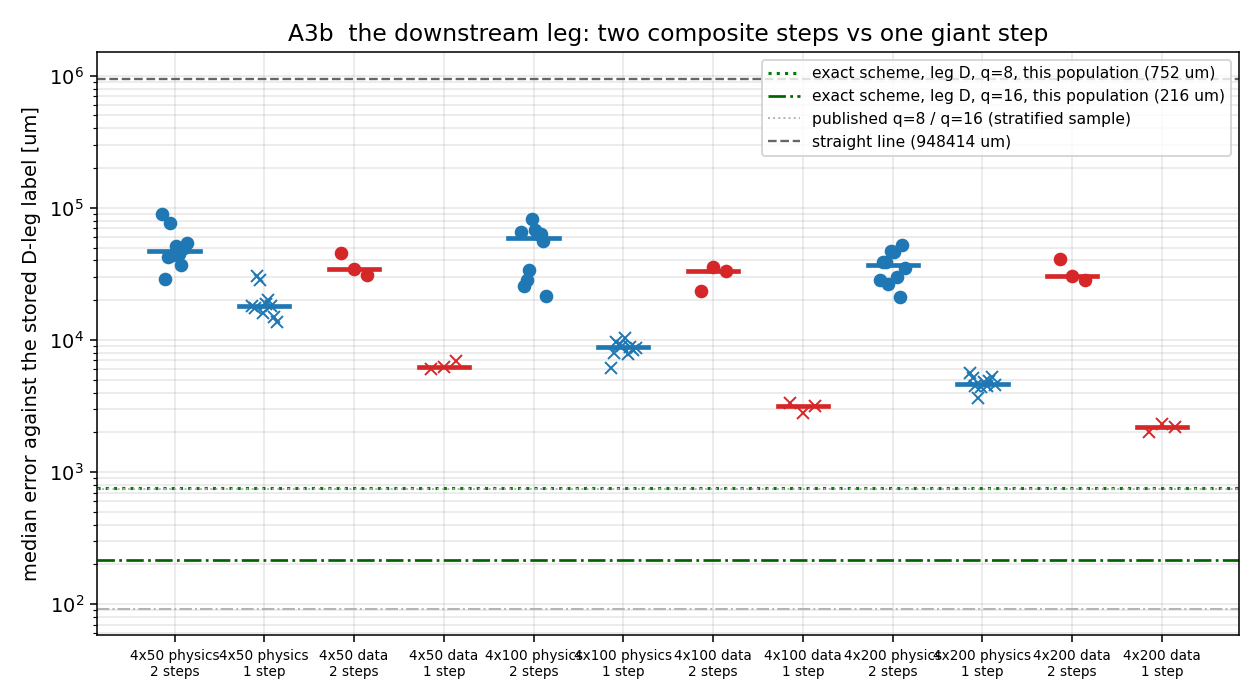
\includegraphics[width=\linewidth]{lhcb_leg_d.png}
      \srcnote{Leg D, the single backward step of median length $-8.6$ m from
        the first post-magnet plane to the collision vertex, a geometry that
        appears in no training set. Left: the error distribution for the
        composite route and for the single giant step, with the ceiling and the
        straight line marked. Right: the same against momentum.}
      \vspace{-2mm}
      {\footnotesize \bad{The composite route, which was supposed to replace a
       hard step by two easier ones, is worse than the single step at every
       momentum}, because its first hop is longer than any leg in training.}
    \end{column}
  \end{columns}
\end{frame}

% ---- 48 ------------------------------------------------------------------
\begin{frame}[shrink=25]{The straight-line-residual redesign: the two short legs transform, the magnet crossing does not}
  \vspace{2mm}
  \centering\small
  \begin{tabular}{@{}lrrrrrrr@{}}
    \toprule
    & \multicolumn{2}{c}{absolute, physics} & \multicolumn{2}{c}{residual, physics}
    & residual & & \\
    \cmidrule(lr){2-3}\cmidrule(lr){4-5}
    leg & $4{\times}100$ & $4{\times}200$ & $4{\times}100$ & $4{\times}50$ & twin & straight & ceiling \\
    \midrule
    A vertex fetch  & $404$ [$286$--$538$]    & $229$ [$201$--$277$]
                    & \hl{$4.4$} [$2$--$6$]   & $4.1$ [$3$--$6$]
                    & $0.058$ & $10.9$ & $0.0013$ \\
    B cross-magnet  & $2600$ [$2106$--$3152$] & $1740$ [$1632$--$2154$]
                    & \bad{$1026$} [$878$--$1209$] & $1136$ [$945$--$1627$]
                    & $512$ & $444{,}075$ & $46.4$ \\
    C plane-to-plane& $300$ [$252$--$335$]    & $213$ [$165$--$235$]
                    & \hl{$1.6$} [$1$--$2$]   & $1.2$ [$1$--$1$]
                    & $0.012$ & $6.6$ & $5.8\times10^{-7}$ \\
    \bottomrule
  \end{tabular}
  \vspace{2mm}

  \centering\small
  \begin{tabular}{@{}lrrrrrr@{}}
    \multicolumn{7}{c}{\textbf{whole test split, all leg types pooled; the straight line on this split is $16.1\um$}}\\
    \toprule
    & \multicolumn{3}{c}{physics loss} & \multicolumn{3}{c}{data twin} \\
    \cmidrule(lr){2-4}\cmidrule(lr){5-7}
    output design & $4\times50$ & $4\times100$ & $4\times200$ & $4\times50$ & $4\times100$ & $4\times200$ \\
    \midrule
    absolute states & $721$ & $397$ & $273$ & $637$ & $321$ & $237$ \\
    straight-line residual & \hl{$2.12$} & \hl{$2.64$} & not run & $0.06$ & $0.04$ & not run \\
    \bottomrule
  \end{tabular}
  \vspace{2mm}

  {\scriptsize Exactly one thing changed: what the network outputs. The dataset
   is byte for byte the same population plus three scale arrays per split; the
   physics loss, the optimiser protocol, the stage count, the splits, the
   momentum bands, the scorer and the ceilings are all unchanged. The one
   deliberate consequential change is that the twin's normalisation follows,
   dividing by the per-sample residual scale, because otherwise it would be
   trained on an objective the physics arm is not. $26$ runs, all $26$
   converged.}
\end{frame}


% ---- 49 ------------------------------------------------------------------
\begin{frame}[shrink=25]{Reading the redesign across, and what the untrained network already scores}
  \vspace{1mm}
  \begin{columns}[T]
    \begin{column}{0.5\textwidth}
      \begin{enumerate}\small
        \item \hl{The two short legs are transformed.} Leg A $404 \to 4.4\um$, a
              factor $92$; leg C $300 \to 1.6\um$, a factor $190$. Both now sit
              \emph{below} the straight line, by $2.5$ and $4$, where the
              absolute design sat thirty to fifty times above it. That is the
              hypothesis's own prediction.
        \item \bad{The cross-magnet leg improves by only a factor $2.5$}, $2600
              \to 1026\um$. Real, but an order of magnitude short of the same
              transformation. Leg B is the one leg where the absolute scale was
              roughly right, so it had least to gain. The redesign fixed a
              conditioning problem, and what is left on leg B is not one.
        \item \hl{Width has stopped mattering} on A and C: $4\times50$ and
              $4\times100$ are within $20$ percent, and the \emph{narrower}
              network is the better of the two on both. The absolute-output
              verdict read the width trend as evidence that width was the
              binding constraint. It was never width.
      \end{enumerate}
    \end{column}
    \begin{column}{0.48\textwidth}
      \begin{enumerate}\small
        \setcounter{enumi}{3}
        \item \hl{The twin is extraordinary on the short legs}, $0.058$ and
              $0.012\um$, four orders better than the absolute twin on each, and
              still twice as good as the physics loss on leg B.
        \item \hl{Distance to the ceiling, the honest scorecard.} The residual
              $4\times100$ physics network is $3400$ times above the ceiling on
              A, $22$ on B and $2.7\times10^{6}$ on C. The absolute factors were
              $310{,}000$, $56$ and $5\times10^{8}$. \bad{The network is nowhere
              near the scheme it is solving on any leg}, and on the short legs
              the scheme is so nearly exact that no network will reach it.
      \end{enumerate}
      \smallskip
      \fbox{\parbox{0.93\textwidth}{\footnotesize
        \textbf{The initialisation check, run before any farm time.} The
        straight-line term agrees with an independent construction to
        $4.5\times10^{-13}\mm$; zeroing the last layer makes output minus
        straight line exactly $0.0\mm$; at the trainer's own initialisation the
        raw output has median $0.057$ in units of the residual scale, which is
        $0.51\um$ at the median endpoint. \hl{An untrained residual network
        already scores $15.5\um$ on the whole test split, against $16.1$ for a
        straight line}, where the converged absolute networks scored about
        $300$. \emph{And the optimisation got easier}: stalls at $40$ to $64$
        restarts against $84$ to $121$, at a loss an order of magnitude lower;
        three of $26$ needed resubmission against $20$ of the first $26$.}}
    \end{column}
  \end{columns}
\end{frame}

% ---- 50 ------------------------------------------------------------------
\begin{frame}[shrink=25]{Where the error lives inside the step, and the tails that did not follow the medians}
  \vspace{1mm}
  \begin{columns}[T]
    \begin{column}{0.55\textwidth}
      \centering\scriptsize
      \begin{tabular}{@{}lrrrrrrrrr@{}}
        \toprule
        & node 1 & 2 & 3 & 4 & 5 & 6 & 7 & 8 & endpoint \\
        \midrule
        absolute, leg A & $365$ & $340$ & $353$ & $320$ & $312$ & $408$ & $349$ & $381$ & $404$ \\
        residual, leg A & $0.06$ & $0.10$ & $0.43$ & $1.01$ & $1.74$ & $2.81$ & $3.64$ & $4.34$ & $4.42$ \\
        \midrule
        absolute, leg C & $289$ & $240$ & $249$ & $270$ & $260$ & $271$ & $268$ & $278$ & $300$ \\
        residual, leg C & $0.03$ & $0.05$ & $0.29$ & $0.65$ & $0.88$ & $1.12$ & $1.34$ & $1.52$ & $1.57$ \\
        \midrule
        absolute, leg B & $987$ & $905$ & $1054$ & $1436$ & $1907$ & $2326$ & $2536$ & $2519$ & $2600$ \\
        residual, leg B & $108$ & $143$ & $277$ & $456$ & $616$ & $812$ & $924$ & $988$ & $1026$ \\
        \bottomrule
      \end{tabular}
      \smallskip

      {\scriptsize Median position error at each Gauss node and at the endpoint,
       test split, $4\times100$ physics loss, median over seeds, $\mu$m.}
      \smallskip

      {\small \hl{This is the clearest single piece of evidence that the
       diagnosis was right.} A flat profile means the error is present before
       any physics has happened, so it is an offset. A rising profile means it
       is accumulated along the step. The absolute error on A and C is flat; the
       residual error rises by a factor $50$ to $70$ from a very small first
       node. Leg B kept its monotonic growth and simply scaled down by $2.5$.}
    \end{column}
    \begin{column}{0.43\textwidth}
      \centering\scriptsize
      \begin{tabular}{@{}lrrrr@{}}
        \multicolumn{5}{c}{\textbf{95th percentiles, $4\times100$, all momenta}}\\
        \toprule
        leg & abs. physics & resid. physics & abs. twin & resid. twin \\
        \midrule
        A & $30{,}693$ & $23{,}640$ & $10{,}445$ & \bad{$20{,}128$} \\
        B & $41{,}542$ & $27{,}080$ & $18{,}395$ & $17{,}425$ \\
        C & $2862$     & \hl{$292$} & $2193$     & \hl{$32$} \\
        \bottomrule
      \end{tabular}
      \smallskip

      {\small \bad{A small population got worse while the bulk got thousands of
       times better.} Those are the soft tracks that bend hardest. The residual
       scale is a first-order estimate, and where the true deviation is many
       times that estimate the network is back to writing down a large number.
       The residual twin's tail on leg A is \emph{twice} the absolute twin's.
       \smallskip

       Fixing the median did not fix the tail, and \hl{the tail is what an
       extrapolator with a bounded time budget actually has to survive.}}
    \end{column}
  \end{columns}
\end{frame}

% ---- 51b -----------------------------------------------------------------
\begin{frame}[shrink=25]{The redesign in pictures: crossing the straight line, and an offset becoming an accumulation}
  \vspace{1mm}
  \begin{columns}[T]
    \begin{column}{0.42\textwidth}
      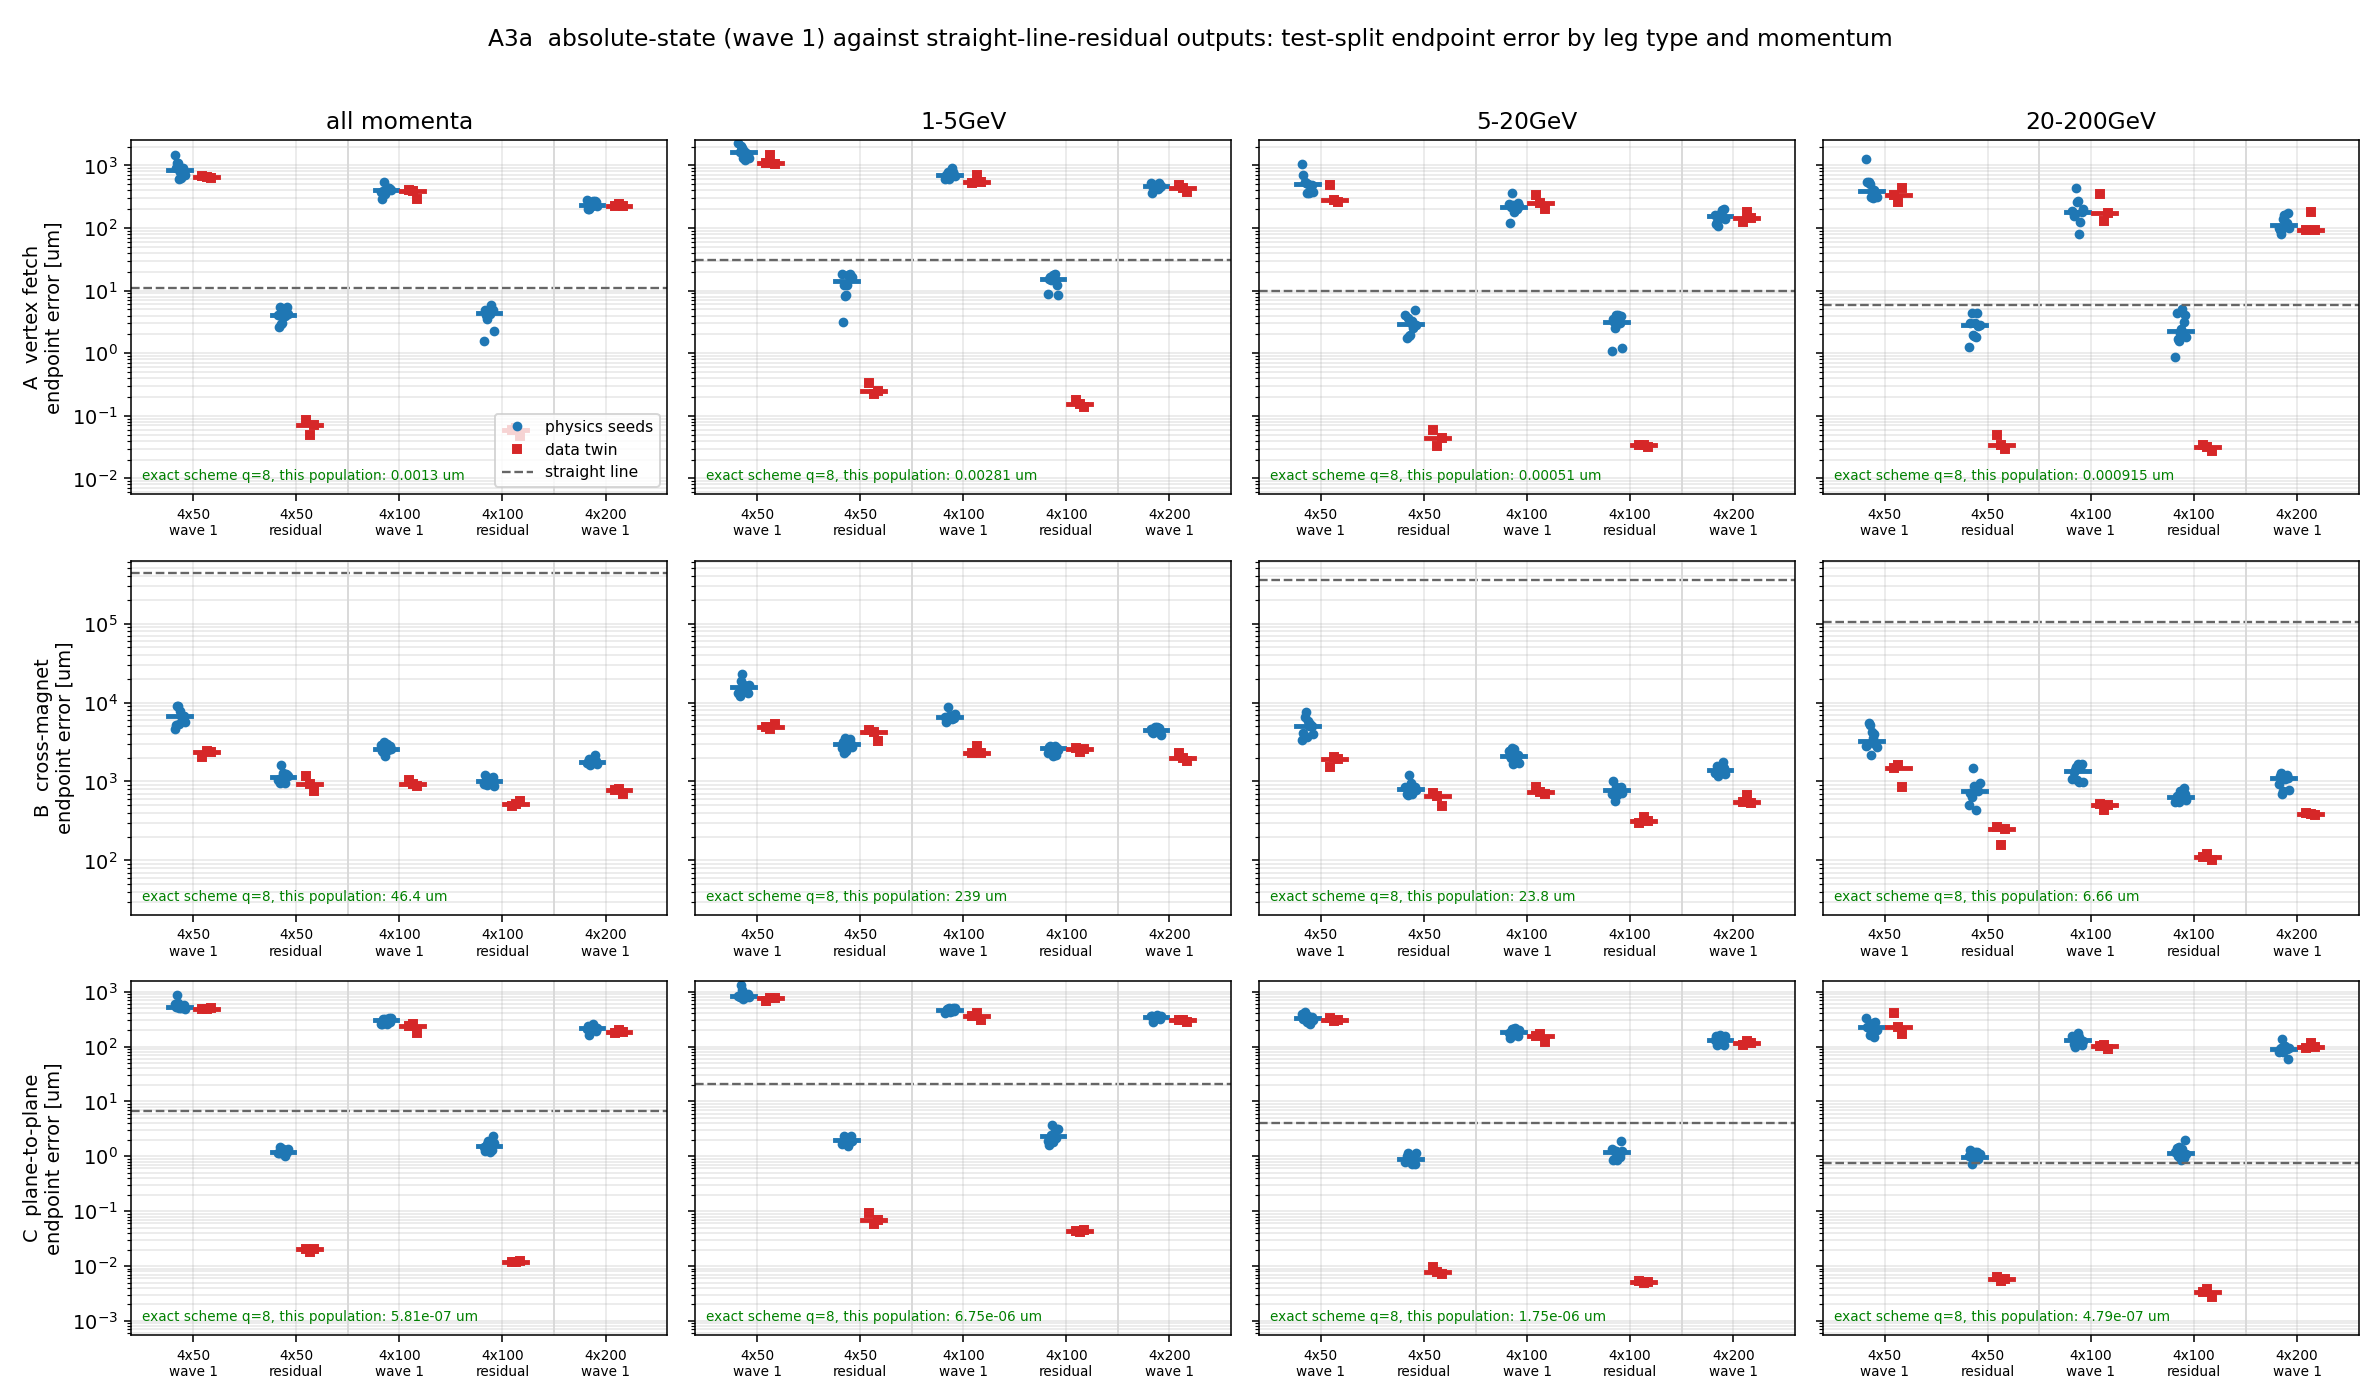
\includegraphics[width=\linewidth]{lhcb_residual_legs.png}
      \srcnote{The same layout as the absolute-output figure, with the residual
        arm added. Rows are leg types, columns momentum bands. The
        absolute-output seeds are the upper cloud in each panel and the residual
        seeds the lower one. \hl{On the top and bottom rows the residual cloud
        crosses from above the straight line to below it}, which is the whole
        point of the redesign; on the middle row it moves down by a factor
        $2.5$ and stays well above both the ceiling and its own twin. The
        improvement on the short legs is uniform in momentum, a factor $46$ to
        $200$ in every band, so it is not an artefact of the momentum mix.}
    \end{column}
    \begin{column}{0.56\textwidth}
      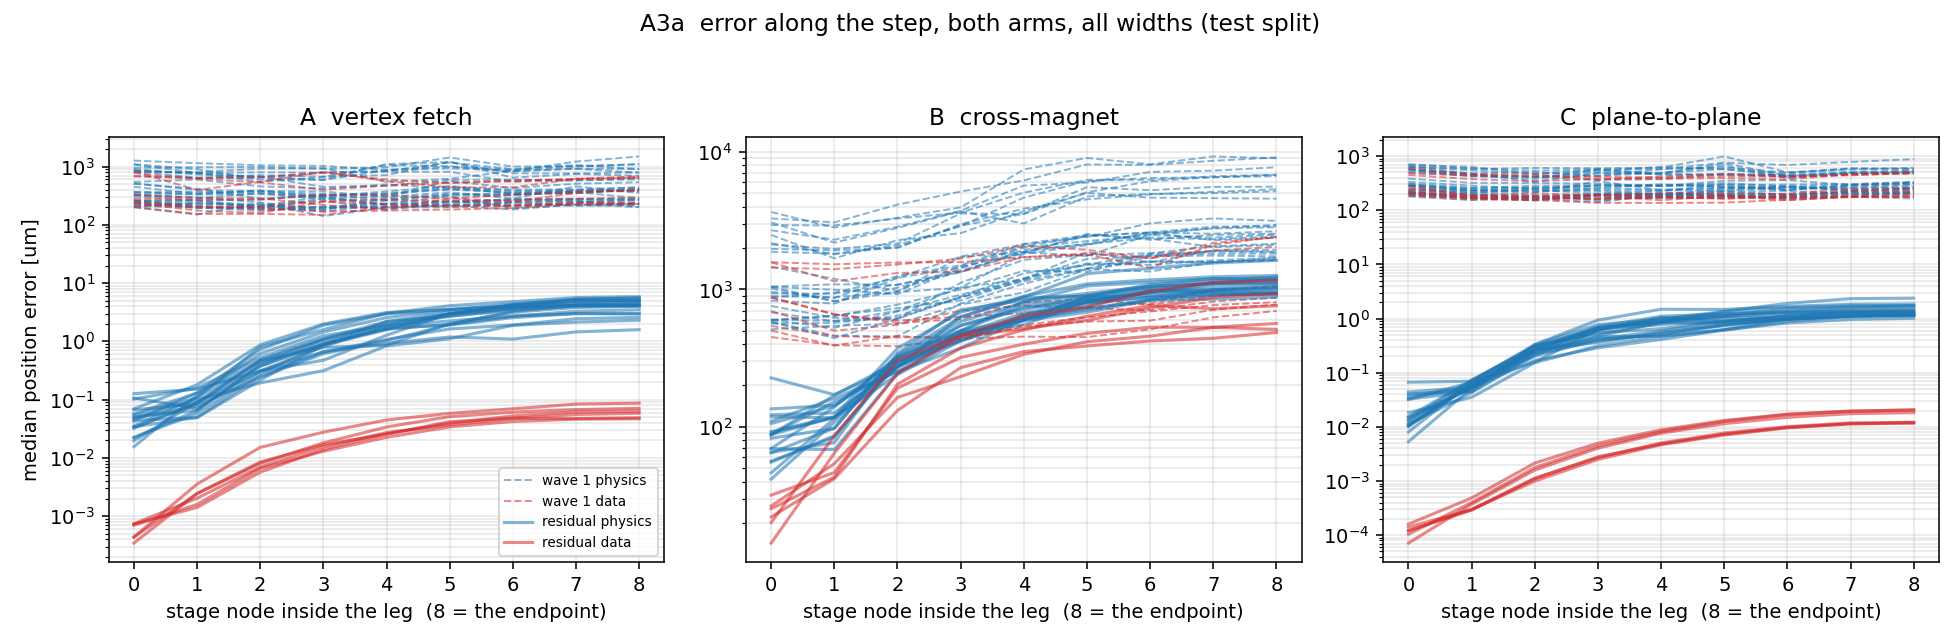
\includegraphics[width=\linewidth]{lhcb_residual_stages.png}
      \srcnote{The error along the step, both output designs, one panel per leg
        type. Horizontal axis: the eight Gauss--Legendre nodes and then the
        endpoint. Vertical axis: median position error in micrometres,
        logarithmic.}
      \vspace{-2mm}
      {\small \hl{A flat profile means the error is present before any physics
       has happened}, so it is an offset the network cannot resolve at the
       population scale. \hl{A rising profile means it is accumulated along the
       step.} The absolute-output curves on the two short legs are flat; the
       residual curves rise steeply from a very small first node. The
       cross-magnet leg kept its monotonic growth in both designs and simply
       scaled down by $2.5$, which is the signature of a bend still being
       under-resolved rather than of an offset.
       \smallskip

       The one cell where the residual network is still worse than a straight
       line is plane-to-plane at $20$ to $200$ GeV, $1.2$ against $0.74\um$: a
       stiff $70\mm$ hop is so nearly straight that there is essentially nothing
       to predict, and the network's own noise floor is above the thing it is
       correcting.}
    \end{column}
  \end{columns}
\end{frame}

% ---- 51 ------------------------------------------------------------------
\begin{frame}[shrink=25]{Chaining the residual networks: better everywhere, and compounding faster}
  \vspace{2mm}
  \centering\small
  \begin{tabular}{@{}crrrrrr@{}}
    \toprule
    legs & \multicolumn{2}{c}{absolute $4{\times}100$} & \multicolumn{3}{c}{residual} & \\
    \cmidrule(lr){2-3}\cmidrule(lr){4-6}
    walked & physics & twin & $4{\times}100$ & $4{\times}100$ twin & $4{\times}50$ & particles \\
    \midrule
    $1$ & $246$      & $217$  & \hl{$1.2$}  & $0.01$ & $1.1$  & $4563$ \\
    $2$ & $783$      & $652$  & \hl{$60$}   & $2.7$  & $59$   & $4563$ \\
    $3$ & $1443$     & $1051$ & \hl{$281$}  & $32$   & $261$  & $4563$ \\
    $4$ & $2293$     & $1484$ & \hl{$572$}  & $118$  & $568$  & $4563$ \\
    $5$ & $4831$     & $2869$ & $1750$      & $471$  & $1919$ & $2914$ \\
    $6$ & $8904$     & $4820$ & $3804$      & $1052$ & $3973$ & $1481$ \\
    $7$ & $10{,}248$ & $5284$ & $4492$      & $1259$ & $4739$ & $853$ \\
    \bottomrule
  \end{tabular}
  \vspace{2mm}

  \begin{columns}[T]
    \begin{column}{0.48\textwidth}
      {\small \hl{The chain is better everywhere.} After four legs the residual
       network is $4.0$ times better with the physics loss, $572$ against
       $2293\um$, and $12.6$ times better with the twin. Over a full seven-leg
       path it is still $2.3$ and $4.2$ times better. The 95th percentile
       improves by the same factor at every step, $13.1$ against $38.6\mm$ at
       leg four, so this is the whole distribution moving.
       \smallskip

       \bad{But the compounding got worse.} Growth ratios at $4\times100$ with
       the physics loss: $48.6$, $4.67$, $2.04$, $3.06$, $2.17$, $1.18$, against
       $3.18$, $1.84$, $1.59$, $2.11$, $1.84$, $1.15$ for the absolute design.
       The residual network starts two hundred times lower, at essentially its
       own plane-to-plane number, then multiplies by $49$ on the second leg.}
    \end{column}
    \begin{column}{0.48\textwidth}
      {\small \hl{The reason is visible in the one-step table.} A chain's early
       legs are short hops, where the residual network is at $1.6\um$; its later
       legs include the cross-magnet crossing, where it is at $1026\um$, the leg
       the redesign barely improved. \bad{The chain error is dominated, after
       two or three steps, by the one leg that did not get better.} The redesign
       bought a much better start, not a slower compounding.
       \smallskip

       Seed selection survives: ranking physics seeds by validation chain error
       at four legs and reading out on test gives $0.98$ and $0.90$. The cheap
       alternative improves but is still not usable, $0.72$ at $4\times100$ and
       $0.35$ at $4\times50$, where in the absolute arm it carried no
       information at $0.08$. Ten seeds differ by $60$ percent in chained error
       at fixed architecture.}
    \end{column}
  \end{columns}
\end{frame}


% ---- 52 ------------------------------------------------------------------
\begin{frame}[shrink=25]{The cross-magnet leg across all three designs, on one axis}
  \vspace{1mm}
  \begin{columns}[T]
    \begin{column}{0.52\textwidth}
      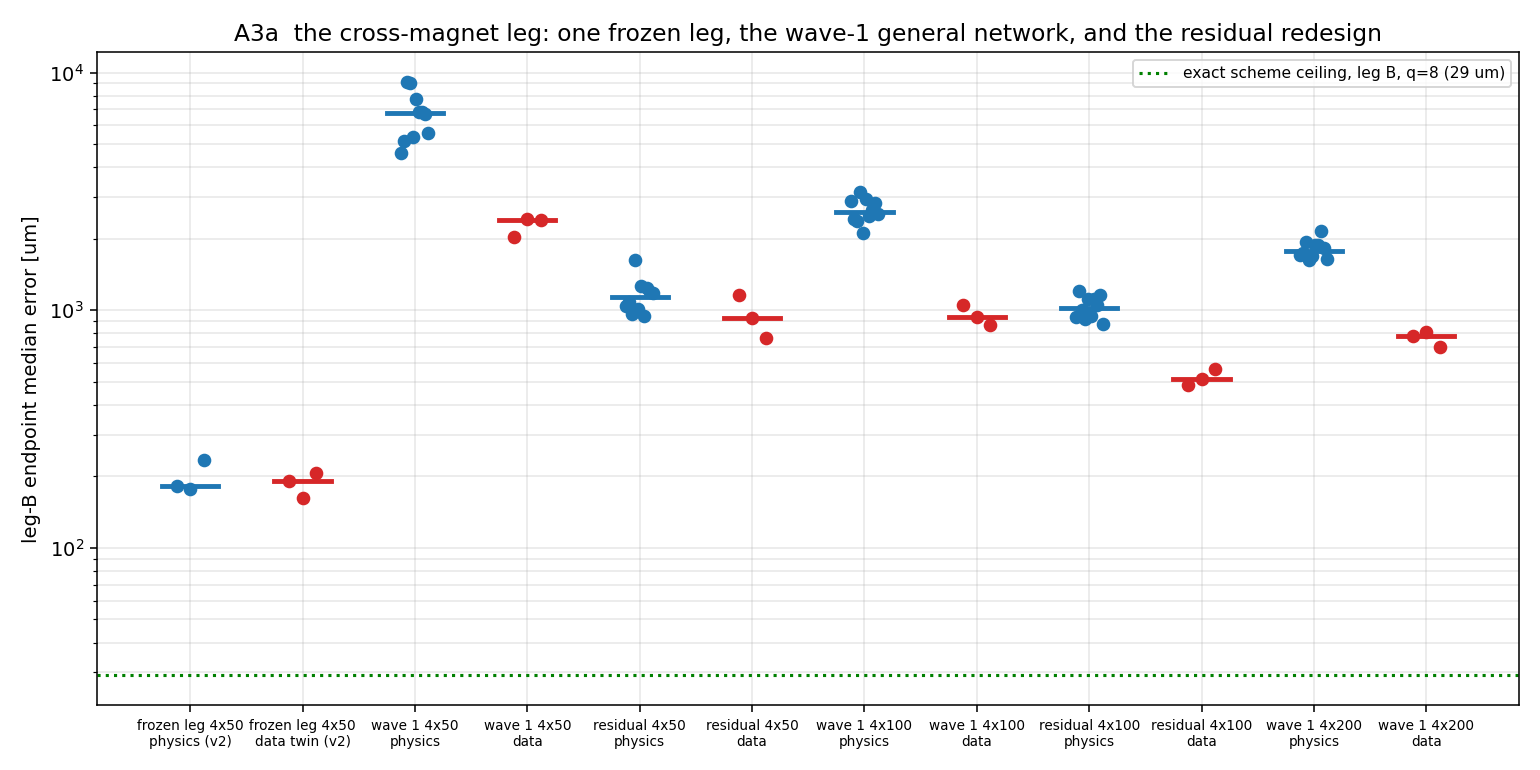
\includegraphics[width=\linewidth]{lhcb_frozen_vs_general.png}
      \srcnote{The frozen-leg network, which trains on that geometry alone; the
        general network with absolute outputs; and the general network with the
        straight-line-residual parameterisation. The exact-scheme ceiling on
        each population and the straight-line baseline are drawn.}
    \end{column}
    \begin{column}{0.46\textwidth}
      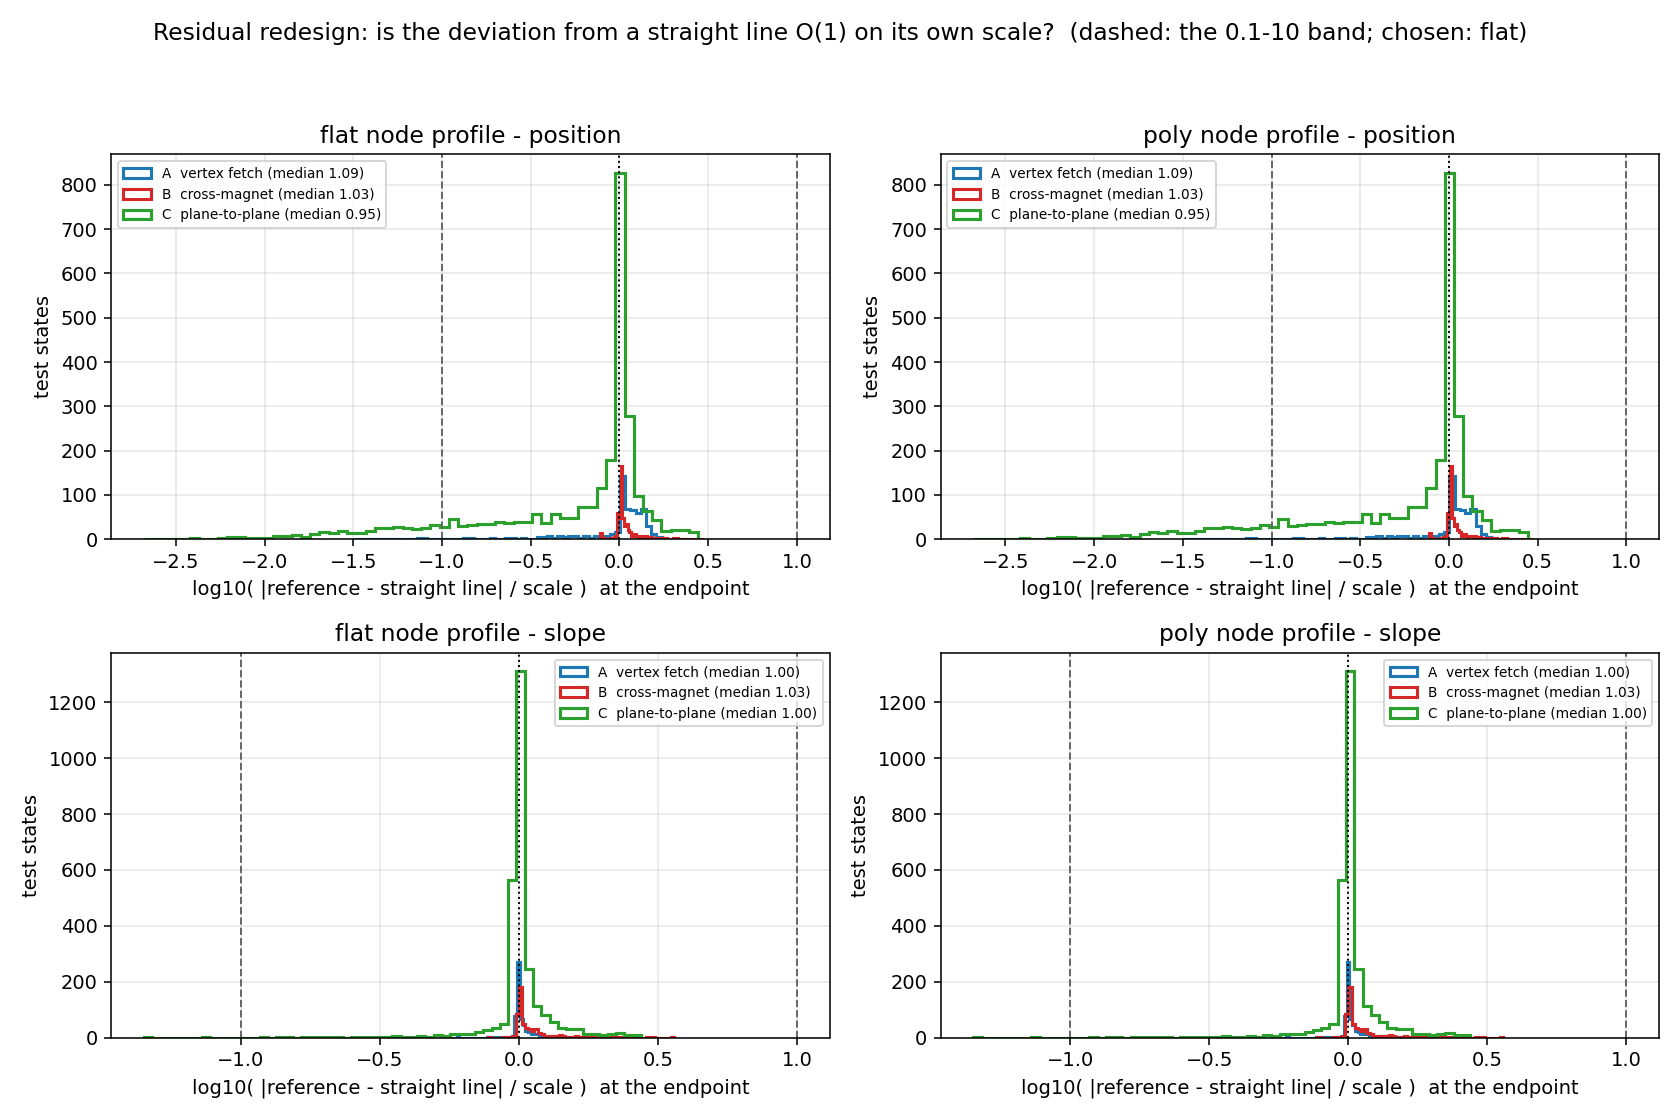
\includegraphics[width=0.9\linewidth]{lhcb_residual_scale.png}
      \srcnote{The check that had to pass before any farm time was spent: the
        distribution, by leg type, of the ratio the network actually has to
        emit, that is the reference deviation from a straight line divided by
        the label-free scale, for both node profiles. Medians $1.09$, $1.03$,
        $0.95$, so the pre-fixed rule selected the flat profile. The same
        label-free expression lands within ten percent of the truth on a
        $341\mm$ backward vertex fetch, a $5.2$ m magnet crossing and a $70\mm$
        sensor hop.}
      \vspace{-2mm}
      {\small \hl{Making the leg an input costs a factor $14$; the residual
       redesign recovers a factor $2.5$ of it.} This gap, and not the output
       scale, is what the next experiments attack.}
    \end{column}
  \end{columns}
\end{frame}

% ---- 53 ------------------------------------------------------------------
\begin{frame}[shrink=25]{The whole programme on one page}
  \vspace{1mm}
  \centering\footnotesize
  \begin{tabular}{@{}lrrrccr@{}}
    \toprule
    & \multicolumn{2}{c}{frozen leg} & magnet up
    & \multicolumn{2}{c}{one network, legs A / B / C, $4\times100$} & chained \\
    \cmidrule(lr){2-3}\cmidrule(lr){5-6}
    & $4\times50$ & $4\times200$ & $4\times50$ & absolute & residual & 4 legs \\
    \midrule
    exact scheme (ceiling)
      & $23$ & $23$ & $22$
      & $0.0013$ / $46$ / $6\!\times\!10^{-7}$
      & $0.0013$ / $46$ / $6\!\times\!10^{-7}$ & n.m. \\
    network, physics loss
      & $222$ & \hl{$115$} & $229$
      & $404$ / $2600$ / $300$
      & \hl{$4.4$ / $1026$ / $1.6$} & $572$ \\
    network, data twin
      & $192$ & $128$ & $204$
      & $385$ / $933$ / $235$
      & $0.058$ / $512$ / $0.012$ & $118$ \\
    straight line
      & $520{,}444$ & $520{,}444$ & $525{,}184$
      & $10.9$ / $444{,}075$ / $6.6$
      & $10.9$ / $444{,}075$ / $6.6$ & n.a. \\
    \midrule
    seed range, physics
      & [$165$--$244$] & [$100$--$134$] & [$171$--$296$]
      & 10 seeds & 10 seeds & selected seed \\
    \bottomrule
  \end{tabular}
  \vspace{1mm}

  {\scriptsize Test-split median endpoint error in $\mu$m. Each column's ceiling
   is measured on that column's own population. The evidence base is $232$
   training runs; $208$ reached a confirmed stall, the $24$ that did not are all
   in the architecture grid at width $32$ or depth $6$, and \hl{no run blew
   up.}}
  \vspace{2mm}

  \begin{columns}[T]
    \begin{column}{0.47\textwidth}
      \fbox{\parbox{0.93\textwidth}{\small
        \hl{Question 1, does it work: yes, on every test.} Training is stable;
        the network sits on the scheme's error to $0.1$ and $0.6$ percent where
        the scheme limits; the shortfall where the network limits is identified
        as optimisation at $+0.965$ over $96$ runs; at $4\times200$ it beats its
        own twin; and it reaches the same floor on a polarity with no labels of
        its own, which is in fact the sample's own polarity.}}
    \end{column}
    \begin{column}{0.47\textwidth}
      \fbox{\parbox{0.93\textwidth}{\small
        \hl{Question 2, can it be used: the redesign changed three of four
        answers.} Short legs went from thirty to fifty times worse than ignoring
        the magnet to two to four times better; the split went $274 \to 2.1\um$
        against $16.1$; the chain improved by $4$ to $13$ at every length;
        composite stepping went from six times worse to $13$ percent worse.
        \bad{What is left is one leg.}}}
    \end{column}
  \end{columns}
  \vspace{2mm}

  {\small\color{warm}\textbf{The cost statement, flagged.} A median of $44$
   root-finder residual evaluations per leg against one forward pass. That is an
   operation count, not a measurement.}
\end{frame}

% =========================================================================
% VII. ISSUES
% =========================================================================

% ---- 54 ------------------------------------------------------------------
\begin{frame}[shrink=25]{Two ceilings and a floor, and the gap between them}
  \vspace{1mm}
  \begin{columns}[T]
    \begin{column}{0.5\textwidth}
      \textbf{1. The $C^0$ field map caps the scheme at $23\um$}
      \begin{itemize}\small
        \item The map is a measured table on an $81 \times 81 \times 146$ grid
              at $100\mm$ spacing, read by trilinear interpolation. The
              interpolant is continuous; its derivative is not. At every cell
              boundary the gradient jumps.
        \item High-order schemes derive their order from Taylor expansions of
              the right-hand side, which require it to be differentiable. It is
              not. A $5178\mm$ crossing passes about $52$ cell boundaries in $z$
              alone, and many more in $x$ as the track bends.
        \item So the ceiling falls from $5401\um$ at $q = 4$ to $23\um$ at
              $q = 8$ and then \emph{stops}, reaching only $20\um$ at $q = 16$:
              the median moved $13$ percent while the unknowns doubled. The tail
              improved much more, $1610 \to 325\um$, consistent with the tail
              being dominated by soft tracks that sample the map most
              aggressively.
        \item \hl{This is not a property of any network.} It is what the
              mathematics being solved is worth on this field map.
      \end{itemize}
    \end{column}
    \begin{column}{0.48\textwidth}
      \textbf{2. The network floor sits a factor $5$ above that}, and it is the
      optimiser: three decades of training loss map monotonically onto one and a
      half decades of error, and every architecture and every seed lies on one
      band.
      \vspace{2mm}

      \textbf{3. The binding constraint is one leg.}
      \begin{itemize}\small
        \item The magnet crossing inside a shared network sits at \bad{$1026\um$
              against a $46\um$ ceiling on its own population}, a factor $22$,
              and the redesign moved it by only $2.5$.
        \item It is not width: $4\times50$ and $4\times100$ agree within ten
              percent on it. It is not the output scale: leg B is the one leg
              where the absolute scale was roughly right.
        \item \hl{The supervised twin is also stuck}, at $512\um$, a factor $11$
              above the ceiling, while reaching $0.058$ and $0.012\um$ on the
              other two legs. Whatever limits leg B limits both losses, so it is
              not a property of the label-free objective.
        \item Cross-magnet legs are \hl{$13$ percent} of the training states;
              plane-to-plane hops are $70$ percent. Under the absolute
              parameterisation the population-wide scale was set by the long legs
              and they dominated the loss anyway. Under the residual
              parameterisation every leg is order one, so the gradient is
              dominated by the easy majority. \bad{The redesign fixed the
              conditioning and, in doing so, handed the optimisation budget to
              the plane-to-plane hops.}
      \end{itemize}
    \end{column}
  \end{columns}
\end{frame}

% ---- 55 ------------------------------------------------------------------
\begin{frame}[shrink=25]{What I cannot claim yet}
  \vspace{2mm}
  \begin{columns}[T]
    \begin{column}{0.5\textwidth}
      \begin{itemize}\setlength{\itemsep}{5pt}\small
        \item \bad{Chaining compounds.} Roughly a factor two per leg in every
              architecture and both losses, and the residual design compounds
              \emph{faster} than the design it replaced. Nothing diverges,
              nothing saturates, and width shifts the curve down without
              changing its slope.
        \item \bad{The tails did not improve with the medians.} On legs A and B
              the residual 95th percentile is no better than the absolute one,
              and the residual twin's tail on leg A is twice as large. A 95th
              percentile of $27\mm$ on the magnet crossing is not usable no
              matter what the median is.
        \item \bad{No throughput benchmark exists.} Everything runs in double
              precision on one core. Nothing here says what the same network
              does in reduced precision on a graphics processing unit, which is
              where it would have to live.
        \item \bad{Labels are free at LHCb.} A reference label is one integrator
              call away, so the label-free advantage is \emph{methodological}
              rather than economic: portability across field maps, geometries
              and conventions. The reversed-polarity test is the demonstration
              of that, and it is the honest form of the claim.
      \end{itemize}
    \end{column}
    \begin{column}{0.48\textwidth}
      \textbf{Harness lessons, recorded so they cost someone else less than they
      cost me}
      \begin{itemize}\small
        \item \hl{The restart cap counted the stall phase and the confirmation
              pass together}, so runs that stalled near the cap were recorded as
              unconverged when they were about to converge. Three experiments
              hit this independently on the same day. The default is raised from
              $150$ to $400$; the cleaner fix, giving the confirmation pass its
              own budget, is not yet applied. No result changes, because a
              larger cap cannot affect a run that stopped on the stall criterion
              below it.
        \item \hl{Ceilings must be quoted on the scored population.} Mixing the
              stratified and natural conventions turns a factor $56$ into $90$
              or $36$, and neither means anything.
        \item \hl{Single thread, and the boundary it creates.} Multithreaded
              PyTorch spin-waits on these nodes and is about $68$ times slower.
              September runs are single-threaded and July runs used four
              threads; a different reduction order changes the last bits and
              $200$ line-searched iterations amplify that into the fourth
              significant digit. Comparisons across that boundary are made at
              the level of seed ranges, never digit for digit.
        \item \hl{One unconverged seed} in the second wave, at $111$ restarts of
              its $400$ cap, resubmitted but caught by a long queue. Reported
              unconverged and excluded from every median; it ranks third on the
              validation chain and does not affect the selection.
      \end{itemize}
    \end{column}
  \end{columns}
\end{frame}

% ---- 56 ------------------------------------------------------------------
\begin{frame}[shrink=25]{What would falsify the edge: two tests with their criteria stated in advance}
  \vspace{1mm}
  \begin{columns}[T]
    \begin{column}{0.5\textwidth}
      \textbf{Test 1: the throughput benchmark}\\[2pt]
      {\small \emph{Design.} The $4\times200$ residual network in single
       precision, batched, against the production extrapolator, on the
       deployment hardware, over the same test population, with both timed
       end to end including the field lookups. Accuracy matched by tuning the
       production integrator's step until its median endpoint error equals the
       network's on that population, so the comparison is not made at a
       different accuracy on each side.}
      \smallskip

      {\footnotesize \hl{Pass.} The network is faster at matched accuracy, and
       its per-batch time has a variance small enough to schedule against, with
       the 99th percentile within a stated factor of the median.}
      \smallskip

      {\footnotesize \bad{Fail.} The network is not faster at matched accuracy;
       or reduced precision costs more accuracy than the accuracy budget allows;
       or the fixed-cost claim does not survive batching, because the production
       integrator amortises better than the operation count suggests.}
      \smallskip

      {\footnotesize \emph{Either way this is the decisive result}, and it is
       currently the largest unmeasured quantity in the programme.}
    \end{column}
    \begin{column}{0.48\textwidth}
      \textbf{Test 2: the cross-magnet-only network}\\[2pt]
      {\small \emph{Design.} Train the residual parameterisation on leg B alone,
       with the start plane and step length still inputs, so the network must
       serve a \emph{family} of magnet crossings rather than one frozen
       geometry. Same protocol, same seeds, same ceiling measured on the same
       population. Its cheaper twin, a stratified training mix over all leg
       types, answers the same question from the other side.}
      \smallskip

      {\footnotesize \hl{Pass, meaning the minority-share explanation is right.}
       It recovers most of the factor $22$, landing within roughly a factor $3$
       of the $46\um$ ceiling. Remedy: a training mix, which is a one-line
       change to the dataset builder.}
      \smallskip

      {\footnotesize \bad{Fail, meaning the leg is genuinely harder.} It stays
       near $1026\um$. Then a $5.2$ m crossing needs more than eight stages or
       more than a first-order scale, and the remedy is in the parameterisation
       or the scheme, not in the data mix.}
      \smallskip

      {\footnotesize \emph{The two outcomes point at different work}, which is
       why this is worth running before anything else on the accuracy side.}
    \end{column}
  \end{columns}
  \vspace{1mm}
  \begin{center}
    \fbox{\parbox{0.9\textwidth}{\footnotesize\color{warm}
      \textbf{And the standing falsifier for the whole product claim:} a 95th
      percentile the trigger cannot budget for. At $27\mm$ on the magnet
      crossing, a median improvement changes nothing about deployability.}}
  \end{center}
\end{frame}

% =========================================================================
% VIII. DIRECTION
% =========================================================================

% ---- 57 ------------------------------------------------------------------
\begin{frame}[shrink=25]{The rest of the queue, in order}
  \vspace{2mm}
  \begin{enumerate}\setlength{\itemsep}{7pt}
    \item \hl{A smoother field surrogate.} The $23\um$ ceiling exists because
      the interpolated map has no continuous derivative, so past $q = 8$ there
      is no smoothness left for extra order to exploit. A smooth surrogate for
      the field, fitted once offline, lifts the ceiling for the scheme and for
      every network trained against it, and removes the reason high order
      currently buys nothing. It also changes what is being solved, which is why
      it is a question for this room and not a decision for me.
    \item \hl{A second-order residual scale.} The first-order estimate is right
      to ten percent at the median and wrong by a large factor on exactly the
      soft, hard-bending tracks that dominate every tail in this work. Folding
      in the curvature of the straight-line path through the field, rather than
      only the field magnitude along it, stays label free because everything it
      needs is still an input.
    \item \hl{Two small items the campaign produced.} The confirmation pass
      should have its own restart budget rather than sharing the stall phase's
      cap. And the exact-scheme solver still hard-wires the magnet-down field
      and had to be copied to measure the reversed-polarity ceiling; it should
      take the field as an argument, the way the derivative function and the
      reference integrator already do.
    \item \hl{Then, and only then, the continuous-time column on LHCb.} The
      decision to open it was parked until the residual redesign had been
      measured, because the redesign addressed the specific failure that would
      otherwise have been the reason to switch. The next slide records what the
      theory predicts there, before rather than after.
  \end{enumerate}
\end{frame}

% ---- 58 ------------------------------------------------------------------
\begin{frame}[shrink=25]{What the stability theory predicts for the continuous-time column on LHCb}
  \vspace{1mm}
  \begin{columns}[T]
    \begin{column}{0.53\textwidth}
      \textbf{Recorded before rather than after}
      \begin{itemize}\small
        \item \hl{There is no isolated fixed point to park on.} The right-hand
              side vanishes only where the slopes vanish and the transverse
              field does too, which for a track moving forward through the
              spectrometer is not a state it can sit at. The failure Rohrhofer
              et al.\ document, and that the regulariser was built to price, has
              no obvious analogue here.
        \item \hl{Flow-following splices should be expected instead.} The splice
              construction needs only that the spliced-in piece solves the
              equation near the collocation points, and the system has a
              five-parameter family of solutions through every plane. A
              candidate that follows the true track for part of the interval and
              a neighbouring track thereafter has the same near-zero empirical
              residual. That is the family my regulariser arms converted parking
              \emph{into}.
        \item \hl{So the intervention to reach for is pseudo-time stepping with
              resampling, not the regulariser.} That ordering is a measured
              result over $240$ converged runs, not a guess.
        \item \hl{The difficulty axes are $I_B$ and the chain length}, in place
              of the number of periods. A continuous-time study here should
              sweep those two and nothing else first.
      \end{itemize}
    \end{column}
    \begin{column}{0.45\textwidth}
      \textbf{How I would frame the whole thing in the thesis}
      \vspace{2mm}

      \fbox{\parbox{0.93\textwidth}{\small
        \hl{The method is validated.} The discrete-time construction transfers
        from a two-state autonomous oscillator with an analytic right-hand side
        to a five-component non-autonomous system with a measured,
        non-differentiable field. It reproduces the scheme it solves where the
        scheme limits; its shortfall where it does not is attributed rather than
        excused; and it works where no labels exist. Two systems with very
        little in common give the same loss-to-error rank correlation, $+0.974$
        and $+0.965$, which I did not expect and cannot explain beyond the
        shared optimiser.}}
      \vspace{3mm}

      \fbox{\parbox{0.93\textwidth}{\small
        \bad{The product edge is unproven.} No throughput measurement exists,
        the tails are not budgetable, and the one step the extrapolator exists
        for sits a factor $22$ above the scheme it is solving with its
        supervised twin a factor $11$. After two or three chained legs that
        single leg dominates everything else. The thesis can carry the first
        claim honestly today. The second is a set of experiments, not a set of
        words.}}
    \end{column}
  \end{columns}
\end{frame}

% ---- 59 ------------------------------------------------------------------
\begin{frame}[shrink=25]{What I would like feedback on}
  \vspace{3mm}
  \begin{enumerate}\setlength{\itemsep}{8pt}
    \item \hl{Is the throughput test worth doing now, or after the magnet leg is
      fixed?} It is the result that decides whether the programme has a product,
      but measuring the throughput of a network that is a factor $22$ from its
      own ceiling may answer a question nobody will care about.
    \item \hl{Is a smooth field surrogate acceptable in principle?} It lifts the
      $23\um$ ceiling for everyone and not only for me, but it changes the thing
      being solved. I would like to know whether that reads as a legitimate move
      or as a change of problem.
    \item \hl{What accuracy and what tail would actually be usable?} Every
      number here is scored against the scheme and against a straight line. I do
      not have a requirement to score against, and a 95th percentile target
      would change which experiments are worth running.
    \item \hl{Is the reversed-polarity result the right way to argue
      portability?} Labels are cheap here, so the claim I am making is that a
      loss which never touches a label is immune to changes of field map,
      geometry and convention. I would like that argument attacked before it
      goes into a thesis.
    \item \hl{How much of the van der Pol failure study belongs in the LHCb
      story?} It is what tells me which continuous-time intervention to reach
      for, and it is the only place the splice mechanism is measured rather than
      cited. But it is a different system and it may read as a detour.
    \item \hl{Is the stratified mix the right first move on leg B, or is it a
      distraction from more stages?} Both are cheap. I have argued myself into
      running the cross-magnet-only test first because its two outcomes point at
      different work, and I would like that reasoning checked.
  \end{enumerate}
\end{frame}

% =========================================================================
% IX. REFERENCE MATERIAL
% =========================================================================

% ---- 60 ------------------------------------------------------------------
\begin{frame}[shrink=25]{Reference: the protocol and the gates, in full}
  \vspace{1mm}
  \begin{columns}[T]
    \begin{column}{0.5\textwidth}
      \textbf{The training protocol, unchanged since the July baseline}
      \begin{enumerate}\scriptsize
        \item Build the dataset; transport training states exactly onto the
              leg's start plane if within $60\mm$ of it; compute the label-free
              scales from the resulting population.
        \item Apply the fiducial requirement: discard any state whose reference
              trajectory leaves the field map.
        \item Initialise a fully connected network with hyperbolic-tangent
              activations, double precision throughout, five inputs (seven for
              the general-leg experiments, carrying the start plane and the step
              length) and $4(q+1)$ outputs.
        \item Train with full-batch L-BFGS, $200$ iterations per restart, strong
              Wolfe line search, history $120$, single-threaded on one core.
        \item \textbf{Stall}: restart until two consecutive restarts each
              improve the training loss by less than one percent.
        \item \textbf{Confirm}: fresh optimiser, curvature history discarded;
              converged only if it re-stalls within two restarts without moving
              the train, validation or test medians by more than one percent.
        \item Score on the held-out test split, which contains no particle that
              appears in training.
      \end{enumerate}
    \end{column}
    \begin{column}{0.48\textwidth}
      \textbf{Three gates on the shared package, all passing}
      \begin{itemize}\scriptsize
        \item \textbf{Vendoring parity.} The copied field-map loader returns
              bit-identical values to the original on $200{,}000$ random in-map
              points: measured difference exactly $0.0$ T, and the map file's
              checksum matches.
        \item \textbf{Differentiable-field parity.} The PyTorch field must agree
              with the numerical original to $10^{-12}$ T. Measured:
              $1.3\times10^{-15}$ T on both polarities.
        \item \textbf{Baseline reproduction.} The generalised code with its
              generalisations switched off reproduces the July baseline bit for
              bit: the same dataset of $1979/2062/2018$ states with identical
              arrays, the same initial parameters, the same losses and
              gradients, and the first optimiser restart landing on the same
              number to the last bit.
      \end{itemize}
      \vspace{2mm}

      {\scriptsize All experiment folders import one shared package, so a
       difference between two experiments is a difference in the experiment and
       never a drifted copy of the physics or the optimiser: field-map loader,
       tableau construction, reference integrator, differentiable field,
       network, losses, dataset builders, scorers and training driver.}
    \end{column}
  \end{columns}
\end{frame}

% ---- 61 ------------------------------------------------------------------
\begin{frame}[shrink=25]{Reference: provenance}
  \vspace{1mm}
  \begin{columns}[T]
    \begin{column}{0.5\textwidth}
      \textbf{Repository and commits}
      {\scriptsize
      \begin{itemize}
        \item \texttt{4fe2491} (5 September 2026): the stage sweep, the
              architecture grid, the reversed-polarity test, the general-leg
              network and the shared package. \textbf{Pushed.}
        \item \texttt{333edf7} (6 September 2026): the residual arm, its
              results, chains and verdict. \textbf{Local, pending push.}
        \item \texttt{29e9928} (6 September 2026): the second wave at
              $4\times200$. \textbf{Local, pending push.}
        \item Van der Pol companion: \texttt{072677a} (the chapter with the
              failure study folded in) and \texttt{e56b168} (the 240-run axes
              study).
      \end{itemize}}
      \vspace{1mm}

      \textbf{Sample and field maps}
      {\scriptsize\\ Official LHCb simulation, 2024 minimum-bias, detector
       description and conditions of 17 October 2023, five of eight files
       mirrored locally ($19$ GB), $200$ events. $323{,}533$ rows split by
       particle $258{,}857 / 32{,}389 / 32{,}287$ with seed $20260718$.
       The conditions tag is magnet-\textbf{up}; every label was computed with
       the magnet-down map.
       Canonical field maps at both polarities, grid $81 \times 81 \times 146$
       at $100\mm$ spacing spanning $(-4000, -4000, -500)$ to
       $(4000, 4000, 14000)\mm$, trilinear interpolation, checksums recorded in
       the paper's provenance appendix.}
    \end{column}
    \begin{column}{0.48\textwidth}
      \textbf{Compute}
      {\scriptsize\\ Nikhef HTCondor, all jobs single-threaded and
       double-precision on one core.
      \begin{itemize}
        \item Stage sweep: cluster \textbf{5781154} ($24$ runs), \textbf{5781162} ($8$ resumed).
        \item Architecture grid: \textbf{5781153} ($120$), continuations
              \textbf{5781167}, \textbf{5781442}, \textbf{5781445}, plus
              \textbf{5781358} ($10$ twin runs).
        \item General-leg, first wave: \textbf{5781158} ($26$) with seven
              resubmission clusters.
        \item General-leg, second wave: \textbf{5781443} ($13$ runs, $12$
              converged) with \textbf{5781566}.
        \item Reversed polarity: \textbf{5781156} ($13$) with \textbf{5781163}
              and \textbf{5781164}.
        \item Residual redesign: \textbf{5781469} ($26$ runs, submitted
              5 September 2026 at 21:14, all $26$ confirmed) with three
              continuation rounds.
      \end{itemize}}
      \vspace{1mm}

      {\scriptsize Every figure in this deck is copied unmodified from the
       corresponding mini-paper's figure directory, which in turn copies it from
       the experiment folder that generated it, from committed result tables
       only. The slide-by-slide figure and number map is in \texttt{README.md}
       next to this source.}
    \end{column}
  \end{columns}
\end{frame}

% ---- 62 ------------------------------------------------------------------
\begin{frame}[shrink=25]{Reference: where the full record lives}
  \vspace{2mm}
  \textbf{The two papers}
  \begin{itemize}\small
    \item \emph{A label-free surrogate for track extrapolation in LHCb: the
      discrete-time physics-informed construction measured against the scheme it
      solves.} 38 pages, 13 figures, 16 tables. Every number traced to a
      committed result file.
    \item \emph{Physics-informed neural networks on the van der Pol
      oscillator.} 48 pages, 37 figures. The van der Pol thesis chapter.
  \end{itemize}
  \vspace{3mm}

  \textbf{The five LHCb write-ups}
  {\small
  \begin{itemize}
    \item Overview, July to September:
      \url{https://app.notion.com/p/3d25d544b9d981bc9b6befc96d06dc4e}
    \item Stage-count sweep:
      \url{https://app.notion.com/p/3d25d544b9d981b3922bfbbea66889f4}
    \item Network size and seed:
      \url{https://app.notion.com/p/3d25d544b9d98151ba5de91f44d99447}
    \item One network for all leg types:
      \url{https://app.notion.com/p/3d25d544b9d981759a84cf138afaa0f7}
    \item Reversed magnet polarity:
      \url{https://app.notion.com/p/3d25d544b9d981888b46e46af43b2928}
  \end{itemize}}
  \vspace{3mm}

  {\small Code and committed result tables:
   \url{https://github.com/GeorgeWilliam1999/LHCb-Extrapolation}. Datasets and
   model weights are not committed; they regenerate from the scripts, the
   recorded seeds and the committed metadata. Every figure is regenerated by its
   experiment folder's plotting script from committed CSV tables only.}
\end{frame}

\end{document}
